\documentclass[a4paper,twoside,12pt]{article}

\usepackage[T1]{fontenc}
\usepackage[utf8]{inputenc}
\usepackage[french]{babel}
\frenchbsetup{og=«, fg=»}
\usepackage{tocbibind}
\pagenumbering{arabic}

\usepackage{xcolor}
\definecolor{lightgray}{gray}{0.95}

\usepackage{soul}
\usepackage{minted}

\usepackage[babel]{csquotes}

\usepackage[backend=biber, sorting=nyt, style=enc, autocite=footnote]{biblatex}
\addbibresource{biblio.bib}

\usepackage{hyperref}
\usepackage[stable]{footmisc}

\usepackage[margin=2.5cm]{geometry}
\usepackage{setspace}
\setlength{\parskip}{0em}
\setlength{\parindent}{1cm}
\onehalfspacing

\usepackage{array}
\usepackage{tabularx}
\usepackage{makecell}
\usepackage{booktabs}
\usepackage{longtable}
\usepackage{varwidth}
\usepackage{ragged2e}
\usepackage{multirow}
\usepackage{enumitem}
\setlist{nosep}

\usepackage{graphicx}
\usepackage[export]{adjustbox}
\graphicspath{./images/}
\usepackage{caption}
\usepackage[capitalize]{cleveref}
%\usepackage{subfig}
\usepackage{subfigure}
\usepackage{wrapfig}
\usepackage{float}



%%% Les index
%\usepackage{makeidx}
%\usepackage{multind} %Ou splitidx
%\usepackage{index} %…
%\makeindex
%\makeindex{edition}
%\makeindex{texte}
%\newindex{etude}{adx}{and}{Index de l'étude}
%\newindex{edition}{bdx}{bnd}{Index de l'édition}



%%%Édition critique
%\usepackage{eledmac}
%\usepackage{eledpar}

%\footparagraph{A}

%\renewcommand{\Rlineflag}{D}




\title{Vers la lecture distante du climat}
\author{Krister Kruusmaa}
\date{Juin 2021}


\begin{document}


%\begin{abstract}


\begin{titlepage}
\begin{center}

\bigskip

\begin{large}
UNIVERSITÉ PARIS, SCIENCES \& LETTRES
\end{large}
%TODO: nom établissement de préparation
\begin{center}\rule{2cm}{0.02cm}\end{center}

\bigskip
\bigskip
\bigskip
\begin{Large}
\textbf{Krister Kruusmaa}\\
\end{Large}
\begin{normalsize} \textit{licencié en histoire}\\
\end{normalsize}

\bigskip
\bigskip
\bigskip
\bigskip
\bigskip
\bigskip
\bigskip

\begin{Huge}
\textbf{VERS UNE LECTURE DISTANTE DU CLIMAT}\\
\end{Huge}
\bigskip
\begin{LARGE}
\textbf{EXTRACTION DES PHÉNOMÈNES MÉTÉOROLOGIQUES DES JOURNAUX NUMÉRISÉS DU 19\textsuperscript{e} SIÈCLE}\\
\end{LARGE}

\bigskip
\bigskip
\begin{large}
\end{large}
\vfill

\begin{large}
Mémoire de première année de master\\
\og Humanités numériques et computationnelles \fg{} \\
\bigskip
2021
\end{large}

\end{center}
\end{titlepage}

\thispagestyle{empty}

\section*{Résumé}
\addcontentsline{toc}{section}{Résumé}

L'objectif de ce mémoire est de détecter automatiquement les phénomènes météorologiques à partir de journaux numérisés du 19ème siècle des pays baltes. Des approches numériques comme le traitement automatique des langues, la reconnaissance d'entités nommées et la désambiguïsation d'entités nommées sont testées sur un corpus d'environ 33 000 articles numérisés provenant des collections de la Bibliothèque nationale de Lettonie. Un modèle capable d'extraire des événements météorologiques, des noms de lieux, des dates et des noms de personnes avec un \textit{F-score} de 80\% est présenté, ainsi qu'un prototype de géolocalisation des noms de lieux. Les résultats sont analysés dans la perspective plus large de l'histoire du climat et serviront de base à de futures recherches sur le sujet.

\medskip

\textbf{Mots-clés:} histoire du climat; humanités numériques; reconnaissance d'entités nommées; journaux; pays baltes; Estonie; Lettonie; allemand; 19\textsuperscript{e} siècle.

\textbf{Informations bibliographiques:} Krister Kruusmaa, \textit{Vers une lecture distante du climat: Extraction des phénomènes météorologiques des journaux numérisés du 19\textsuperscript{e} siècle}, mémoire de master 1 \og Humanités numériques et computationnelles\fg{}, dir. Mm. Carmen Brando, M. Jawad Daheur, Université Paris, Sciences \& Lettres, 2018.


\section*{Abstract}
\addcontentsline{toc}{section}{Abstract}

The goal of this thesis is to automatically detect weather phenomena from digitised 19th century journals of the Baltic countries. Digital approaches like Natural Language Processing, Named Entity Recognition and Named Entity Linking are tested on a corpus of about 33 000 digitised articles from the collections of the National Library of Latvia. A model capable of extracting weather events, placenames, dates and peoples' names with a F-score of 80\% is demonstrated, as well as a prototype for geolocalising the place names. The results are analysed in the wider perspective of climate history and will serve as a baseline for future research on the topic.

\medskip

\textbf{Keywords:} climate history; digital humanities; named entity recognition; journals; Baltic countries; Estonia; Latvia; German; 19\textsuperscript{th} century.

\textbf{Bibliographic Information:} Krister Kruusmaa, \textit{Towards a Distant Lecture of the Climate: Extraction of weather phenomena from digitized 19\textsuperscript{th} century journals}, 1\textsuperscript{st} year M.A. thesis  \og Digital and computational humanities\fg{}, dir. Carmen Brando, Jawad Daheur, Université Paris, Sciences \& Lettres, 2018.

\null\newpage
\thispagestyle{empty}
\null\newpage

\section*{Introduction}
\addcontentsline{toc}{section}{Introduction}
\setcounter{page}{1}


L'objectif de ce mini-mémoire est d'expérimenter l'application de méthodes numériques d'extraction d'information et de technologie linguistique pour contribuer au domaine de l'histoire du climat. Plus précisément, un large corpus de journaux numérisés du 19ème siècle sera utilisé pour entraîner un modèle de reconnaissance d'entités nommées (NER) capable de détecter automatiquement des phénomènes météorologiques à partir de textes narratifs en langue allemande. En outre, un prototype de désambiguïsation sémantique d'entités nommées sera présenté, qui est capable de relier les noms de lieux trouvés dans le corpus à des coordonnées géographiques spécifiques, servant ainsi de point de départ à une analyse spatiale du climat.

L'inspiration pour ce projet est venue de la participation de l'auteur à deux projets de recherche à l'Université de Tallinn en Estonie : \textit{Storms - Climate Extremes in Estonia and their Impact on Society} et \textit{Estonian Environmentalism in the 20th Century: Ideology, Discourses, Practices}. Les objectifs de ces projets ont été de cartographier les sources historiques disponibles dans les pays baltes qui contiennent des informations précieuses sur le climat et de réaliser différentes reconstructions du climat du passé. Du point de vue estonien, cet effort peut en partie être considéré comme la continuation des travaux d'Andres Tarand (né en 1940), géographe et l'un des climatologues les plus éminents d'Estonie, qui a passé plus de 20 ans à rassembler différentes sources d'archives et de presse pour créer une première base de données sur l'histoire du climat en Estonie. Aujourd'hui, sous la direction d'Ulrike Plath, professeur d'études gérmano-baltes et d'histoire de l'environnement, les sources rassemblées par Tarand ont été élargies pour inclure des sources de Lettonie, qui appartenait à la même unité culturelle et politique que l'Estonie à l'époque moderne. À l'échelle internationale, les travaux menés à l'université de Tallinn ont des liens étroits avec l'université de Berne et l'équipe de climatologues de cette dernière, dirigée par les professeurs Christian Pfister et Christian Rohr. Les recherches menées à Tallinn utilisent le format et les directives de la base de données Euro-Climhist de l'université de Berne. Nos données seront également incluses dans un module spécial pour la Baltique dans cette vaste base de données.

Un autre objectif de ces projets de recherche est l'application des approches numériques à l'histoire du climat, ce qui est également l'objet de ce mémoire. Il convient de noter qu'il existe toujours un écart très important entre les sources historiques et la modélisation mathématique du climat passé. Cela signifie que les résultats préliminaires qui sont présentés dans ce mémoire ne visent pas à dire quoi que ce soit de concluant sur les tendances générales du climat dans la région baltique. Il s'agit plutôt d'un travail à une échelle élémentaire qui espère fournir une base de référence pour faciliter le processus très exigeant d'analyse des sources qui est nécessaire en histoire du climat. Dans les pages suivantes, un aperçu général du domaine de l'histoire du climat sera donné, ainsi qu'un bref résumé de l'histoire de la région balte, afin d'expliquer la nature des sources.

\begin{figure}[h]
    \centering
    \includegraphics[width=0.7\textwidth]{images/workflow.png}
    \caption{Diagramme des étapes de travail en M1 et M2}
    \label{fig:workflow}
\end{figure}


Le mémoire est divisé en trois chapitres principaux. Dans le premier, une description détaillée du corpus sera donnée, ainsi qu'une discussion sur les possibilités et les limites des données. Le deuxième chapitre décrit le processus de création d'un modèle NER pour l'extraction automatique des phénomènes météorologiques et présente les résultats de ses performances. Le troisième chapitre traite de la question de la spatialité et démontre le processus de réduction de l'ambiguïté des noms de lieux et leur visualisation sur une carte.

Initialement, il était également prévu d'inclure une étude sur la modélisation thématique LDA des sources. Le code de cette approche était déjà écrit, mais aucun résultat significatif n'a été obtenu dans l'immédiat. Compte tenu de cela et du fait que la longueur de cette étude avait déjà atteint ses limites, le chapitre a été laissé de côté, pour être repris l'année prochaine.

Les références sont listées dans la bibliographie. Tous les scripts et \textit{notebooks} se trouvent sur la page GitHub du projet\footnote{\url{https://github.com/krkryger/clim-dist}} et seront mentionnés dans les notes de bas de page.




\subsection*{Histoire du climat}
\addcontentsline{toc}{subsection}{Histoire du climat}


L'histoire du climat, souvent aussi appelé la climatologie historique, est un champ de recherche entre les humanités et les sciences naturelles qui a fait son apparition sous sa forme moderne dans les années 1970.\footcite[Les origines de l'histoire du climat dépendent de la définition que l'on donne au terme \og climat \fg{} qui a subi une transformation importante pendant l'époque moderne. Il est vrai que les savants européens s'ont occupe de la question du temps, l'atmosphère etc. et leur influence sur l'humain déjà depuis de l'antiquité, mais le manque d'une distinction nette entre les aspects physiques et astrologiques, etc. du temps rend difficile l'examination du domaine comme une tradition continue de recherche. Pour une histoire longue de la climatologie, cf. l'excellente synthèse de Franz Mauelshagen dans][]{white_palgrave_2018} L'histoire du climat emploie deux approches pour reconstruire le climat, notamment celles de la paléoclimatologie et celles de la climatologie historique. Ce dernier porte uniquement sur les sources crées par les humains, tandis que le premier s'occupe des \og archives de a nature \fg{}, c'est-à-dire les cernes d'arbres, les glaciers etc.\footcite[][2]{white_palgrave_2018} Les questions de recherche de l'histoire du climat sont diverses :
\vspace{1ex}
\begin{itemize}[label=$\bullet$]
    \item l'état et les changements du temps et du climat depuis la dernière période glaciaire;
    \item l'impact du climat sur les variations de l'agriculture, les conflits sociaux, la santé et la migration;
    \item études de cas sur les périodes d'une variabilité climatique exceptionnelle et leurs impacts;
    \item l'histoire des idées climatologiques et de la science du climat.\footcite[][1-2]{white_palgrave_2018}
\end{itemize}
\vspace{1ex}

Ces directions sont bien visibles dans la recherche des dernières décennies. L'un des axes principales de la recherche est la reconstruction de la température et la pression atmosphérique\footcites{jones_monthly_1999}{camuffo_daily_2002}{camuffo_daily_2002-1}{camuffo_daily_2002-2}, de la précipitation\footcites{fenby_rainfall_2013}, de la fréquence des tempêtes\footcites{jones_preliminary_2005}{barring_scandinavian_2004}{wheeler_atmospheric_2010}{von_storch_storm_2008} etc. avec l'aide des observations instrumentales ou des sources narratives. Le deuxième axe porte plutôt sur des événements discrets, c'est-à-dire des phénomènes singulières de la météo qui peuvent avoir une influence considérable sur la société humaine mais également nous renseigner quant aux meilleures façons de faire face aux extrémités climatiques.\footcites{fredriksson_using_2018}{wheeler_great_2003}{garnier_historical_2018}{brazdil_chronology_2000}{pfister_meteorological_2010}

Un autre composant principale de l'histoire du climat est le recours aux données systématisées et numériques. Emmanuel Le Roy Ladurie, le premier historien d'utiliser des techniques computationnelles et une approche quantitative afin de tirer des conclusions sur l'état du climat de jadis, a lancé ses recherches climatiques avec l'œuvre \og Histoire du climat depuis l'an mil \fg{} qui a p. ex. contribué à la dissémination du concept du petit âge glaciaire.\footcites{le_roy_ladurie_histoire_1967}[Ladurie a continu de s'occuper du climat après dans les années 2000 :][]{le_roy_ladurie_abrege_2007}{le_roy_ladurie_canicules_2005}{le_roy_ladurie_disettes_2006}{le_roy_ladurie_rechauffement_2009} Les travaux de Le Roy Ladurie ont été le plus directement continus par le géographe et historien suisse Christian Pfister, créateur d'une des premières bases de données climatiques, l'Euro-Climhist.\footcite[][]{pfister_christian_euro-climhist_2015} Le Roy Ladurie a loué son travail de ramassage des données et l'application des approches quantitatives et qualitatives en disant : \og En ce qui concerne l’histoire du climat, l’usage qu’a fait Christian Pfister de l’informatique lui a permis de rassembler une quantité de données qui eût été inimaginable autrefois \fg{}.\footcite[168]{le_roy_ladurie_vie_2014}

L'histoire du climat a donc des proches relations au monde numérique dès le début - les compétences de l'historien doivent être combinés avec la mathématique et la programmation pour arriver aux résultats cohérents à partir de la masse hétérogène des sources historiques qui ne se soumit que très involontairement à l'interprétation. Les bases de données sont abondantes dans le domaine - il en existe à différents échelles et buts, par exemple : CLIWOC (\textit{Climatological Database for the World's Oceans}) \footcite{konnen_description_2005}; \textit{The Global Volcanism Program}\footnote{\url{https://volcano.si.edu/}}; Tambora (\textit{The Climate and Environmental History Collaborative Research Environment})\footnote{\url{https://www.tambora.org/}}. Ce que toutes ces bases de données ont en commun est le charge de travail nécessaire pour les créer. Aucune reconstruction du climat du passé n'est possible sans une grande quantité des données (p. ex., 287,114 journaux de bord ont été traités à la main pour réaliser le CLIWOC), mais chaque information venant des sources historiques a besoin d'une approche rigoureuse pour la convertir à l'encodage standardisé de telle ou telle base de données et la rendre quantifiable et comparable aux autres sources. Le développement des gros projets de l'histoire du climat implique donc un très grand nombre des participants.
Bien qu'il existe des approches du \textit{crowdsourcing} pour collecter des données\footnote{\url{https://www.oldweather.org/index.html}}, le grand volume de travail et les incompatibilités résultant de la multitude des différents standards et collections de données sont reconnus par des chercheurs.\footcite{veale_dealing_2017}

Il est notable que les méthodes numériques ont toujours été présentes dans le domaine de la climatologie historique, mais apparemment jamais pour le processus de la collection de données elle-même. L'approche qualitative et individuelle aux sources historiques est probablement considérée tellement importante pour ne pas influencer les résultats, que n'importe quelle approche automatisée semble de risquer de rendre le travail inutile. Ce travail de M1 a donc pour but d'explorer les possibilités du repérage automatique de l'information climatique dans des sources numérisées. L'attente n'est dans aucun cas de réaliser une base complète et prête pour reconstruire un tel ou tel élément du climat du passé, mais plutôt de faire les premiers pas vers la facilitation du travail dans le domaine.



\subsection*{Contexte historique des sources}
\addcontentsline{toc}{subsection}{Contexte historique des sources}


Les sources utilisés pour ce mini-mémoire sont des journaux numérisés du 19\textsuperscript{e} siècle en langue allemand. Pour clarifier ce choix et leur contexte, il vaudrait donner un aperçu court de la région concerné et son histoire. Pour ce qui concerne ce mémoire dans sa portée temporelle, les pays baltes sont considérés comme les trois gouvernements dits Baltes de l'empire Russe : Estonie, Livonie et Curonie (\textit{Estland, Livland, Kurland}). Leurs frontières demeuraient inchangées pendant le 19\textsuperscript{e} siècle et leur territoire correspondait approximativement à celui des Republiques d'Estonie et Lettonie contemporaines situés dans le nord-est de l'Europe, sur la côté est de la mer baltique.\footcites[Pour un aperçu général de l'histoire de cette région, cf.][]{champonnois_estoniens_2004}{kasekamp_history_2018} Il convient de souligner que la Lituanie, le troisième des pays souvent appelés \og baltes \fg{} aujourd'hui, avaient historiquement moins en commun avec les autres deux. Les gouvernements d'Estonie, Livonie et Curonie de l'époque moderne coïncident avec la Livonie médiévale ou \textit{Terra Mariana}, une confédération lâche formée après les Croisades baltes au 13e siècle.\footcites[Une présentation critique de ces événements se trouve dans][]{murray_clash_2009}{selart_livland_2017} Au cours de ces croisades, les croisés et marchands, provenant majoritairement du Saint-Empire romain germanique, ont jeté les fondements politiques et sociales de la région pour les sept siècles à venir - une société chrétienne et culturellement européenne, mais en même temps semi-coloniale, caractérisée par la domination politique et économique d'un groupe sociale peu nombreux qui se distinguait des peuples indigènes (dont les Estoniens, Lives, Coures, Latgaliens, Séloniens et Sémigaliens) avec l'usage de la langue allemande.

\begin{figure}[!h]
\begin{minipage}[b]{0.5\textwidth}
    \centering
    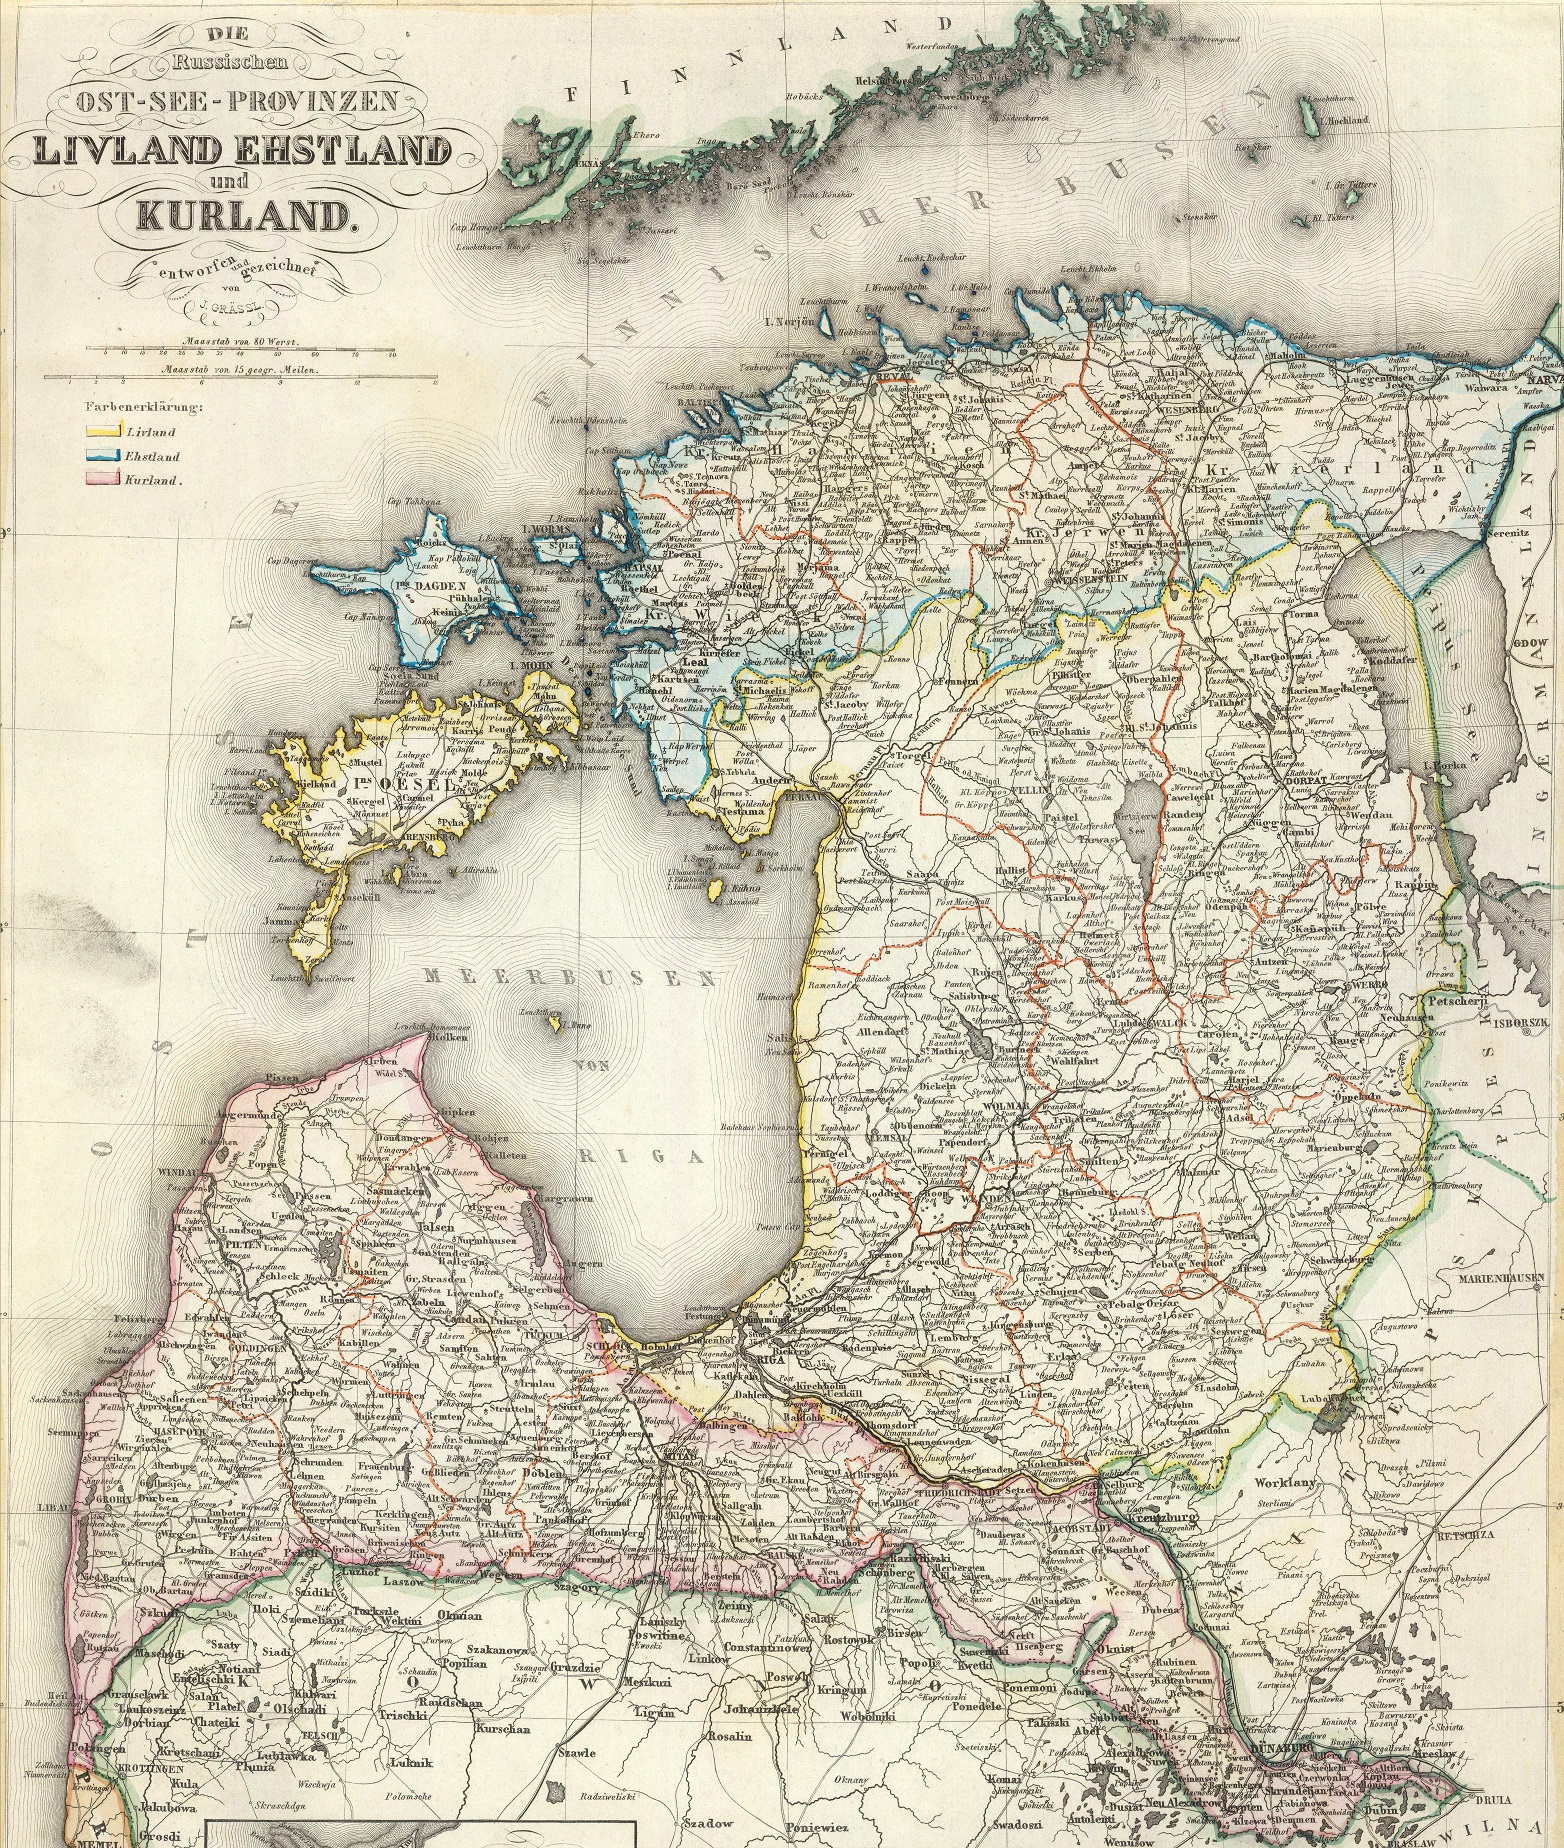
\includegraphics[width=0.9\linewidth]{images/provinces.jpg}
    \captionsetup{width=0.9\linewidth}
    \caption{Les gouvernements d’Estonie, Livonie et Curonie en 1860}
    \label{fig:provinces1860}
\end{minipage}
\begin{minipage}[b]{0.5\textwidth}
    \centering
    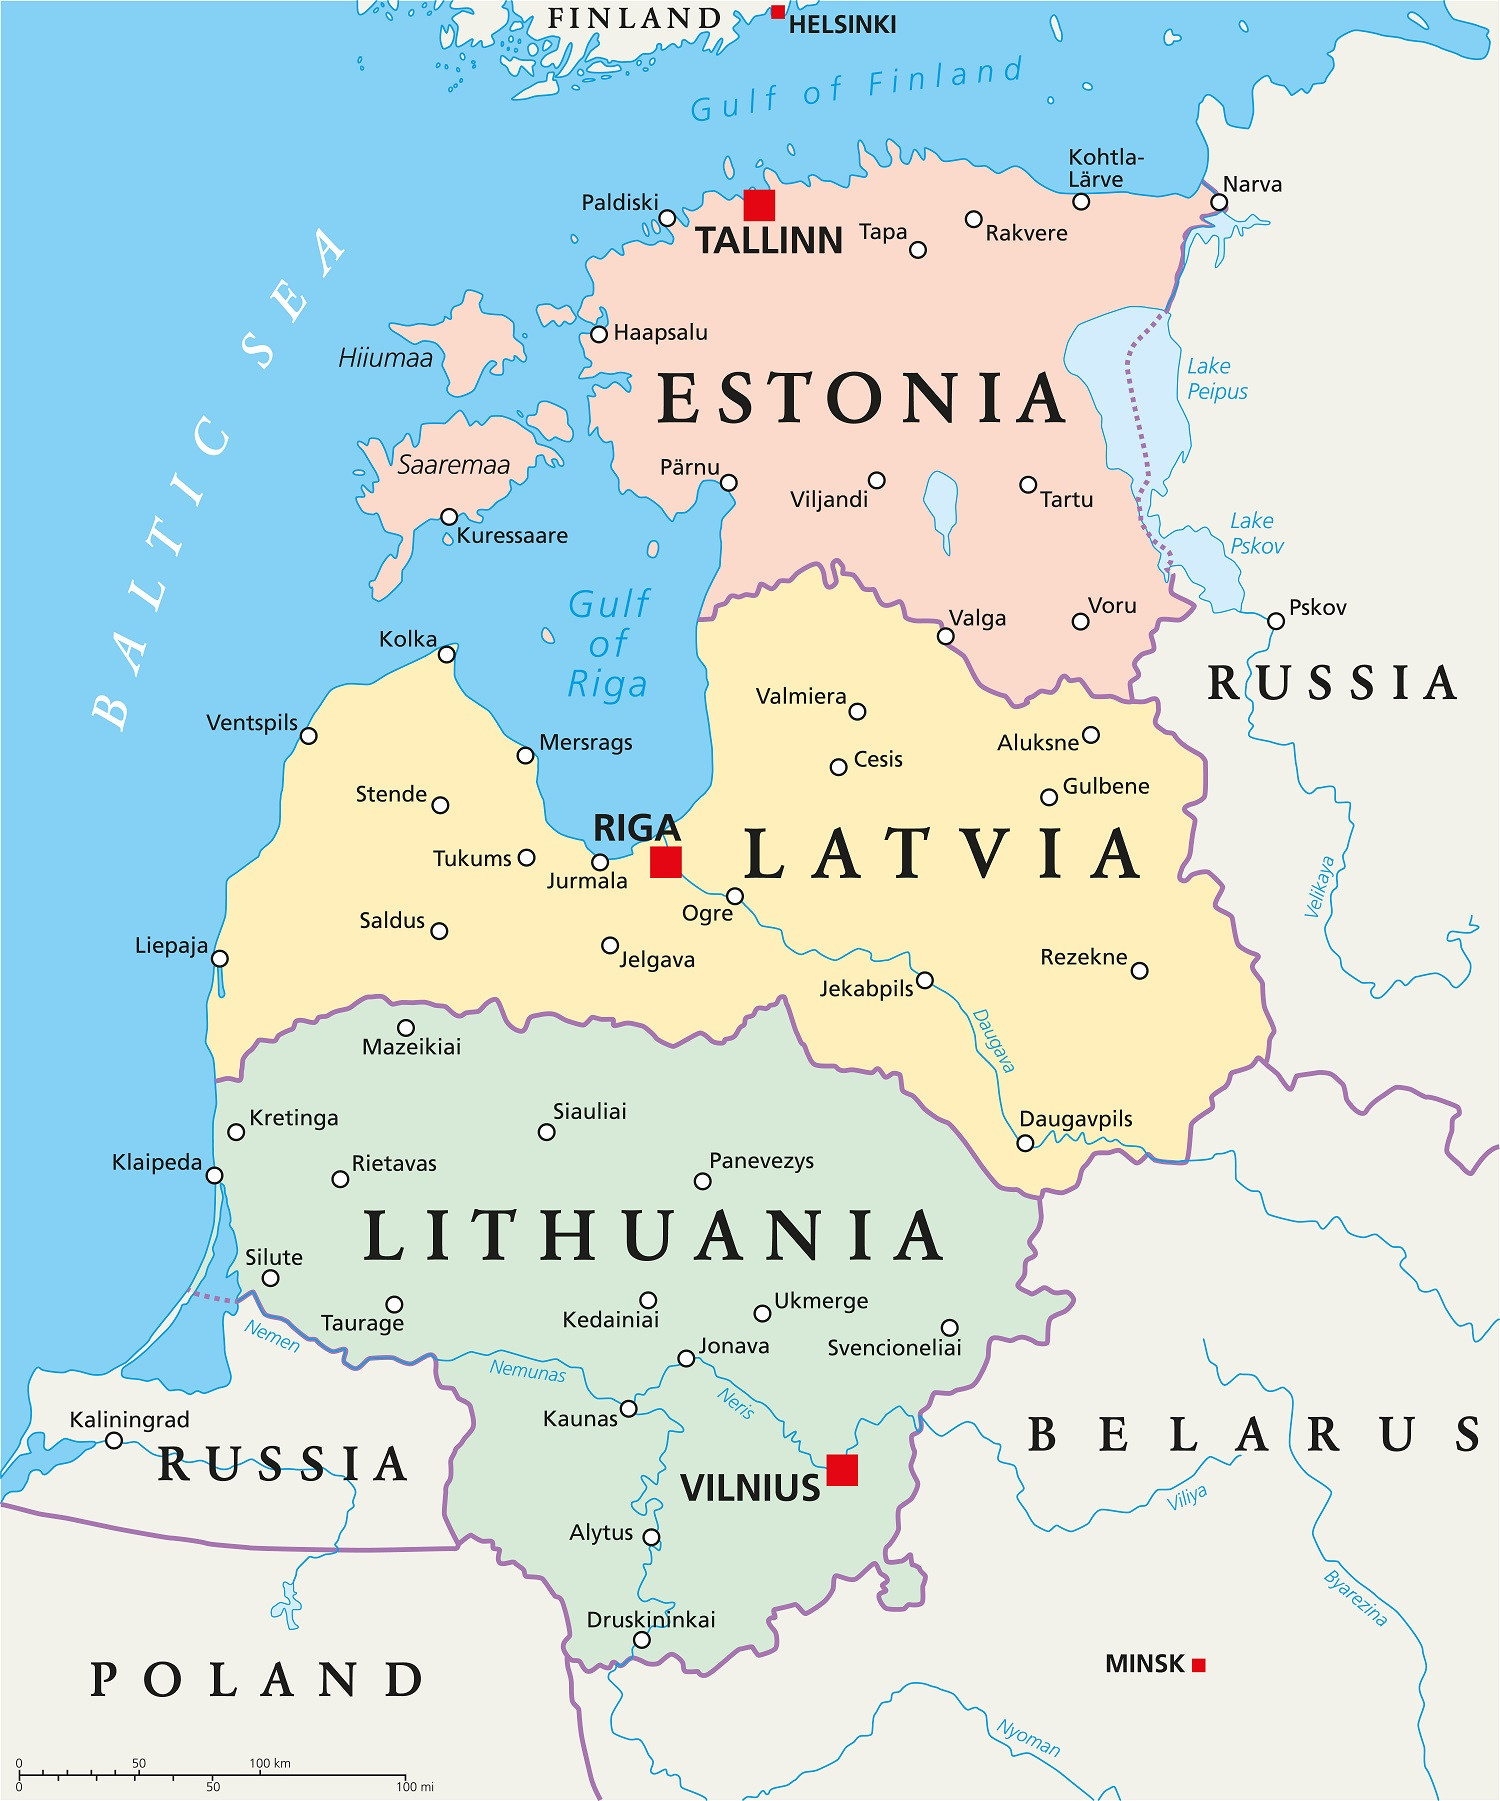
\includegraphics[width=0.9\linewidth]{images/balticcountries.jpg}
    \captionsetup{width=0.9\linewidth}
    \caption{L'Estonie, la Lettonie et la Lituanie aujourd'hui}
    \label{fig:balticcountries}
\end{minipage}
\end{figure}

Même après la dissolution de la Livonie médiévale au milieu du 16e siècle et les dépassements consécutifs de ses territoires entre les gros pouvoirs de la région - la Suède, la Russie et la Pologne -, la situation sociale de la région n'a changé que très peu.\footcites[Paradoxalement, l'allemand reste un élément unifiant à l'époque d'États-nations unitaires, au moins dans le domaine de l'historiographie. Les traitements scientifiques qui prennent en compte la région entière sous la forme et sous les critères qu'elle avait avant le XXe siècle sont ainsi souvent publiés en allemand. Pour les relations internes et externes des pays baltes à partir du Moyen Age jusqu'à la fin du XIXe siècle, cf. p. ex.][]{anton_deutschland_2005}{angermann_baltischen_2015}{muhlpfordt_baltische_2016}{sommerlat-michas_baltikum_2015}{hormuth_livonia_2012} Depuis le 19\textsuperscript{e} siècle, la position de l'élite sociale et de la langue allemande était de plus en plus contestée : d'un côté par les mouvements nationaux des Estoniens et Lettons qui avaient été libérés du servage en 1816-1819, et de l'autre par les ambitions croissantes de la Russie qui tentait d'imposer le russe comme la seule langue administrative dans toutes ses provinces vers la fin du 19\textsuperscript{e} siècle.\footcites[Les tensions culturelles et nationales entre les diverses peuples et minorités de la région, ainsi que leurs relations aux différents pouvoirs politiques externes sont les mieux présentées dans][]{angermann_ostseeprovinzen_2005}{plath_esten_2011} Cela dit, pour la tâche en question, les sources allemandes sont les mieux informées et les plus nombreuses jusqu'aux derniers décennies du siècle, quand ils étaient égalés par la presse estonienne et lettone.

Les journaux allemands, publiés aux grandes et petites villes des gouvernements d'Estonie, Lettonie et Curonie offrent donc les meilleurs possibilités pour étudier le climat. Grâce à son statut en tant que \textit{lingua franca}, l'allemand ouvre une vue géographique et temporelle plus large. L'origine de la presse locale dans les gouvernements Baltes est situé aux années 1680, quand les premières gazettes hebdomadaires et bimensuelles ont parues à Riga et Reval (auj. Tallinn), les deux plus grosses villes baltiques.\footcites[][16-17]{vanamolder_was_2011}{peegel_eesti_1994} Au cours du 18e et du 19\textsuperscript{e} siècle, la masse de la presse a connu une croissance constante. A ses débuts, la presse était considérablement plus concernée par les actualités étrangères, tandis que le 19\textsuperscript{e} siècle a amené un intérêt plus marqué pour les affaires locales et régionales - un élément crucial pour l'étude du climat à cette époque.

En général, les journaux allemands sont le plus volumineux et le plus exhaustives parmi les sources existantes dans les pays baltes, par rapport à l'étude des événements climatiques. Ils sont aussi les plus accessibles, à la différence des documents d'archives qui peuvent bien contenir de l'information sur le climat non parue dans les journaux contemporains, mais qui ne sont pas numérisés dans la mesure où une approche numérique s'emporterait sur les méthodes traditionnelles. Un dernier avantage se manifeste dans la possibilité d'étendre l'approche à d'autres régions historiquement germanophones - ainsi il existe le potentiel de l'évolutivité des solutions trouvés au cours de la recherche.

\clearpage




\section{Sources} \label{sources}

\subsection{Rigasche Zeitung}

???

\subsection{Description du corpus} \label{description_corpus}

Les données utilisées pour ce mémoire proviennent des collections de la Bibliothèque nationale lettone (LNB).\footnote{\url{https://lnb.lv/en}} En comparaison à la Bibliothèque nationale estonienne\footnote{\url{https://nlib.ee/en}} où se trouvent également plusieurs journaux gérmanophones du 19\textsuperscript{e} siècle, leur collection est considérablement plus vaste, car Riga était le centre économique et le capitale \textit{de facto} des gouvernements Baltes. La partie principale de la numérisation des collections de l'LNB a été finie vers 2012. Pour les journaux, les paramètres du balayage étaient JPEG 2000 et 400 dpi. Remarquablement, la segmentation des milliers de pages pour l'océrisation a été faite à la main.\footnote{\url{https://lndb.wordpress.com/2012/06/07/periodikas-digitalizesana-lnb/}}

LNB offre un accès libre à toutes les revues et gazettes du 19\textsuperscript{e} siècle sur la page web periodika.lv\footnote{\url{periodika.lv}}, ainsi qu'un moteur de recherce textuelle pour les transcriptions, mais il n'est pas possible de les télécharger (p. ex. sous la forme d'une API). Par conséquent, il a été nécessaire de contacter la bibliothèque pour recevoir le corpus. Pour le travail de la première année de master, un corpus d'une plus petite taille (ca. 33 000 articles) et avec des critères additionnelles (notamment la présence des certains mots clés météorologiques) a été employé. Ce corpus a été en suite utilisé pour expérimenter des approches différentes, un nombre entre eux ayant trouvé son chemin vers ce travail-ci pour être appliquées à un corpus plus vaste.

Le jeu de données utilisé pour ce mémoire (désormais le corpus) consiste de \textbf{289 704 articles} de la \textit{Rigasche Zeitung} de 1802 à 1888.\footnote{\texttt{./data/external/riga\_zeit\_1802\_1859.parquet \newline ./data/external/riga\_zeit\_1859\_1888.parquet}} Les articles se divisent par 18 499 numéros du journal au cours de 86 ans.\footnote{En fait, il y a 87 années de 1802 à 1888, mais l'an 1882 n'est pas présent dans la base de données de LNB, comme on peut le voir sur les pages suivantes. De ce qui est compris, le journal était bien publié continuellement, car les numéros de l'année précédente et de l'année suivante ne présentent aucun signe d'interruption de publication - il s'agit donc d'une lacune de la numérisation. \label{86_years}} Un aperçu de la distribution des données se présente dans la figure \ref{fig:data_hist}.

\begin{figure}[t]
    \centering
    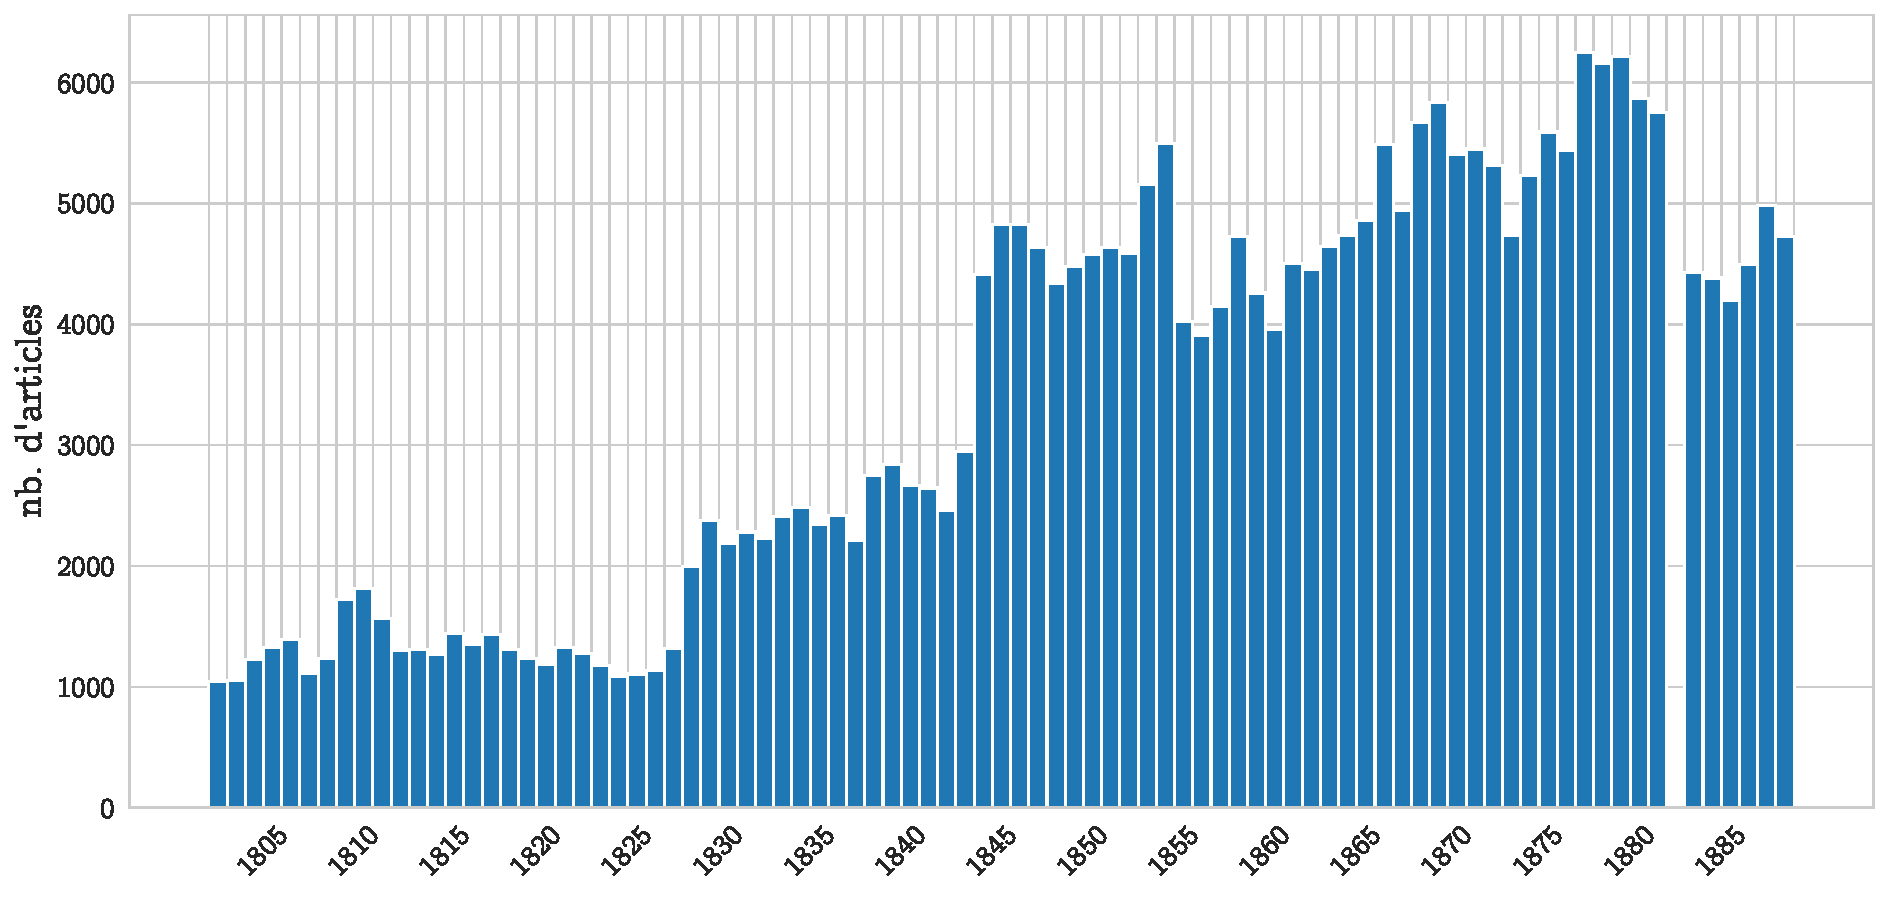
\includegraphics[width=\textwidth]{images/articles_histogram.pdf}
    \caption{Distribution temporelle des données}
    \label{fig:data_hist}
\end{figure}

Dans ce corpus, chaque entrée corréspond à un article et est fournie des caractéristiques suivantes (voir les annexes pour un exemple des données brutes) :

\vspace{1ex}
\begin{itemize}[label=$\bullet$]
    \item \texttt{href} : le lien vers l'article sur \url{periodika.lv} qui permet de vérifier la transcription (mais qui, selon mon expérience précédente avec le site, n'est malheureusement pas permanent et peut être sujet à changement)
    \item \texttt{head} : le titre de l'article
    \item \texttt{date} : la date de publication (selon le calendrier Julien qui était le calendrier officiel de l'Empire russe jusqu'à 1915 en Lettonie et 1918 en Estonie)
    \item \texttt{pub} : le nom de la revue
    \item \texttt{full\_text} : la transcription OCR de l'article entier
    
\end{itemize}
\vspace{1ex}

Enfin, l'index des entrées du corpus brut est utilisé de manière continue tout au long du travail. Cet index, référencé comme \texttt{id}, permet de retracer tout texte jusqu'à sa forme originale au cours des différentes procédures d'analyse, en le reliant à ses métadonnées. Dès lors, les références aux articles du \textit{Rigasche Zeitung} sont accompagnées de ses \texttt{id} correspondants dans les notes de bas de page, ce qui permet de les retrouver plus facilement dans le corpus.

\subsection{Prétraitement}  \label{pretraitement}

Avant de passer à l'analyse thématique, un traitement et nettoyage préliminaire du corpus sont nécessaires. Le prétraitement consiste à générer des caractéristiques supplémentaires pour pouvoir sélectionner et manipulation plus aisément, et à traiter le texte brut en le séparant en mots singuliers pour permettre la vecteurisation et l'analyse des mots-clés.

Le premier prétraitement des données a été réalisé avec la bibliothèque Pandas de Python qui permet de faire toute sorte de manipulation sur des tableaux. Les attributs suivants ont été dérivés à partir des existants et ajoutés au corpus\footnote{\href{https://github.com/krkryger/clim-dist/blob/main/climdist/climdist/data_preprocessing.py}{\texttt{./climdist/data\_preprocess.py}}} :

\vspace{1ex}
\begin{itemize}[label=$\bullet$]
    \item \texttt{year} : l'année
    \item \texttt{month} : le mois
    \item \texttt{day} : le jour
    \item \texttt{text\_len} : le nombre des caractères dans \texttt{full\_text}
\end{itemize}
\vspace{2ex}

\subsubsection{Evaluation de la qualité d'OCR} \label{ocr_quality}

Ensuite, les textes avec une qualité trop faible ont été marquées pour pouvoir les écarter aux stades de l'analyse textuelle. Le tableau \ref{table:ocr} montre une échantillon de texte tel que visible sur le site de LNB et son OCR correspondante (les erreurs sont surlignées en jaune). Bien entendu, la qualité peut varier considérablement entre les textes ou dans un seul texte, mais cet exemple illustre bien certains des problèmes habituels. L'on peut constater plusieurs choses. Premièrement, le journal utilise l'écriture gothique (\textit{Frakturschrift}) qui pose normalement plus de défis pour un moteur OCR.\footcite[Pour un aperçu des problématiques généraux de l'OCR des textes allemands (quoique avec un accent sur les 17e-18e siècles) et pour l'état de l'art autour du moment de la complétion de la numérisation des catalogues de LNB, cf. ][]{federbusch_volltext_2013} Ces difficultés se présentent le plus souvent sous la forme de confusion de \textit{f} avec \textit{s}, et le groupe \textit{m}, \textit{n}, \textit{e}, \textit{tt} et \textit{ii}. En plus, les guillemets \og \fg{} apparaissent souvent sans raison. Deuxièmement, la segmentation des articles et très étroite, un fait qui cause des problèmes aux bouts de lignes. Ainsi, les tirets de césure sont très souvent omis du texte résultat, provoquant beaucoup d'ambiguïté par rapport aux mots composés (omniprésents en allemand). Un autre problème lié à la segmentation n'est pas visible dans l'exemple mais se présente dans le cas d'une mise en page complexe : les limites d'un article peuvent être flous ou se confondre avec des publicités ou d'autres éléments.

\begin{table}[h]
\begin{minipage}[b]{0.415\textwidth}
    \centering
    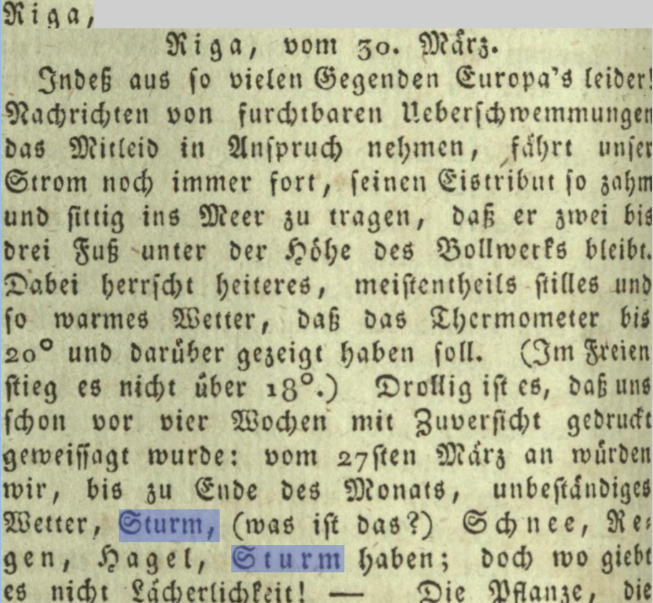
\includegraphics[width=\linewidth]{images/ocr_comparaison.png}
  \end{minipage}
  \hspace{0.05\textwidth}
  \begin{varwidth}[b]{0.5\textwidth}
    \centering
    \scriptsize
      \parbox[b]{\linewidth}{\texttt{Riga\\\\\hl{P}i\hl{s}a, vom \hl{so. Wirst-z. \fg{}} \\ \hl{\fg{} Jtt}deß aus so vielen Gegenden E\hl{n}ropa\hl{w} leider!\\
Nachrichte\hl{tt} von furchtbaren \hl{Il}eberschwe\hl{tnnt}u\hl{tt}gen\\
das Mitleid in Anspruch nehmen, \hl{\fg{}sti}hrt \hl{ti}nse\hl{t}\\
Strom noch immer fort, \hl{f}einen Eistri\hl{lsti}t so zahm\\
und\hl{\fg{}} sittig ins Meer zu tragen, daß er zwei bis\\
drei\hl{\fg{}} Fuß \hl{\fg{}}unter der Höhe des \hl{V}ollwerks bleibt.\\
Dabei herrscht heiteres, meistentheils stilles und\\
so warmes Wetter, daß das Thermo\hl{sn}eter bis\\
\hl{no\fg{}} und darüber gezeigt haben soll. (\hl{Jtn} Freien\\
stieg es nicht über \hl{:80}.) Drollig\hl{\_}ist\hl{\_}es, daß\hl{\_}utts\\
schon vor vier Wochen mit Zuversicht gedruckt\\
geweissagt wurde: vom 27\hl{f}ten M\hl{ei}rz an würden\\
wir, bis zu Ende des \hl{Nk}onat\hl{th} unbes\hl{icktt}diges\\
Wetter, Sturm, (\hl{tv}as ist das?) Schnee, \hl{N\fg{}}\\
gen, Hagel, Sturm haben; d\hl{v}ch w\hl{v} giebt\\
es nicht \hl{\fg{}}Lächerlichkeit! —\hl{\fg{}} Die Pflanze, die}}
  \end{varwidth}%
  \caption{Exemple de la qualité d'océrisation de LNB}
  \label{table:ocr}
\end{table}

La post-correction d'un corpus historique est considérée comme une tâche très ardue, même que le domaine est en plein développement.\footnote{Pour une comparaison d'approches et l'état d'art, cf. Gotscharek Annette, Reffle Ulrich, Ringlstetter Christoph, Schulz Klaus U. et Neumann Andreas, 2011, \og Towards information retrieval on historical document collections: the role of matching procedures and special lexica \fg{}, International Journal on Document Analysis and Recognition (IJDAR), juin 2011, vol. 14, n. 2, p. 159‑171.} Un nettoyage complet des données serait donc hors du champ de ce travail. Il est cependant possible d'arriver à des résultats significatifs en utilisant la taille même du corpus et en reconnaissant ses limitations d'OCR. Au lieu d'attendre une océrisation \og parfaite \fg{}, nous pouvons faire usage des qualités existantes du texte. Pendant des expérimentations, il s'est avéré que les approches de traitement automatique de la langue (\textit{Natural Language Processing}, NLP) ont bien des limitations, mais ils peuvent être utilisés conjointement avec des méthodes \textit{corpus-based}, notamment ceux qui s'appuient sur des vecteurs de mots que nous verrons plus tard.

A place d'une post-correction des textes, j'ai donc décidé d'implémenter un simple algorithme d'apprentissage machine afin de pouvoir écarter les entrées d'une trop mauvaise qualité pour l'étape d'analyse textuelle. Toutes les données sont conservées pendant ce stade, mais chaque entrée est fournie d'une score (\texttt{0} ou \texttt{1}) pour permettre d'établir un taux de \og lisibilité \fg{}. Afin d'entraîner un modèle d'apprentissage supervisé, un nombre de textes sont traités en Python par un modèle de langue allemande développé par SpaCy.\footnote{Pour cette analyse simple et préliminaire, un modèle de base \texttt{de\_core\_news\_md} est utilisé, entraîné sur des textes allemands contemporains. Les détails du modèle se trouvent ici : \url{https://spacy.io/models/de\#de\_core\_news\_md}\label{de_core_news}} Le modèle est utilisé ici pour \textit{tokeniser} le texte, i.e. d'itérer un séquence de caractères et d'en repérer leur structure, en séparant les mots l'un de l'autre et en ajoutant à chaque mot (\textit{token}) des étiquettes qui décrivent leur position morpho-syntaxique. A ce point nous ne nous intéressons qu'aux quantités relatives des différents types de \textit{tokens} dans le texte. Les caractéristiques sélectionnées pour chaque texte, afin de le classifier selon la lisibilité, sont les suivantes :
\vspace{1ex}
\begin{itemize}[label=$\bullet$]
    \item proportions relatives des étiquettes morpho-syntaxiques suivantes: pronom, adverbe, auxiliaire, nombre, verbe, adjectif, espace, ponctuation, inconnu;\footnote{\textit{Ibid.} pour la schéma d'annotation morpho-syntaxique du modèle en question.}
    \item proportion relative de symboles \og inhabituels \fg{}, n'appartenant pas à \textit{a-z}, \textit{A-Z} (y compris les caractères spéciaux \textit{öäüß} de la langue allemande) ou le groupe \mbox{\textit{.,'"?!;-:}}
    \item nombre de caractères divisé par le nombre de \textit{tokens}
\end{itemize}
\vspace{2ex}

Pour apprendre un modèle d'apprentissage machine à distinguer les textes lisibles de ceux qui contiennent trop de bruit ou d'erreurs à partir des caractéristiques nommées, une échantillon aléatoire de 300 textes est sélectionné et chaque texte est évalué. Les textes considérés illisibles sont ceux qui en pratique ne pourraient jamais être proprement traités par l'ordinateur (ou qui ne sont même pas compréhensibles pour l'humain - voir le tableau \ref{tab:readability_example} pour un exemple de texte considéré illisible. Le texte dans le tableau \ref{table:ocr} aurait un score positif).

\begin{table}[h]
\centering
\begin{tabular}{|p{0.9\linewidth}|}
\hline
\vspace{0.5ex}
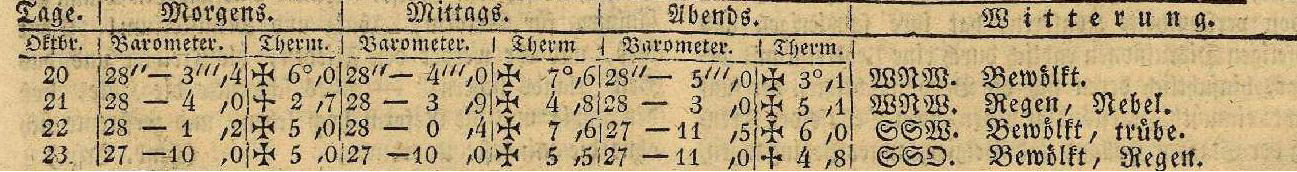
\includegraphics[width={\linewidth}]{images/ocr_quality_example.png} \\
\hline
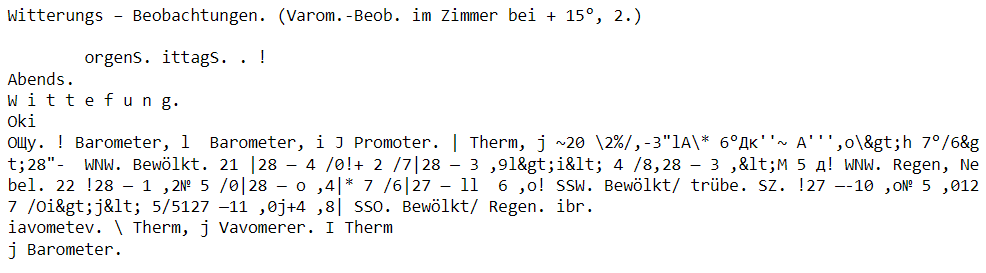
\includegraphics[width={\linewidth}]{images/ocr_quality_example_text.png} \\
\hline
\end{tabular}
\captionsetup{justification=centering}
\caption{Extrait d'un article considéré illisible dans le \textit{ground truth}\\ (RZ 24/10/1831 (\texttt{id: 42181}))}
\label{tab:readability_example}
\end{table}

Les caractéristiques et les annotations pour ces 300 textes sont ensuite utilisées comme les données d'entraînement d'un classificateur de type machine à vecteurs de support (SVM).\footnote{\texttt{./notebooks/ocr\_quality.ipynb}} La machine à vecteurs de support a pour but de projeter chaque point de données dans un espace hyperdimensionnel (dont le nombre de dimensions correspond au nombre de caractéristiques énumérées ci-dessus) et de trouver un hyperplan qui sépare le deux groupes de données (i.e. lisibles et non lisibles) en maximisant la distance entre chaque point d'entrée et l'hyperplan.\footnote{---référence générale pour les SVM}

L'exactitude moyenne atteinte par le modèle s'élève à 87\%, un score dont la signifiance est difficile à évaluer, étant donné la nature subjective du classificateur. La décision sur la lisibilité d'un texte est faite par un algorithme mais elle se pose pourtant sur une élément subjectif, car c'est l'utilisateur qui établit le norme (le soi-disant \textit{ground truth}) que l'algorithme essaie de reproduire.
Il est impossible à établir une frontière bien délimitée entre lisible et non lisible - deux catégories dont la distinction reste intrinsèquement fluide - mais l'on peut dire avec une certaine confiance que l'application du classificateur aide à nettoyer le corpus et la perte de données d'une qualité haute d'OCR est presque inexistante ou inexistante.\footnote{Le classificateur se trouve dans \texttt{./data/models/ocr\_quality\_model\_150921/}, le script pour l'appliquer à tout le corpus et générer la colonne de lisibilité est \texttt{./climdist/ocr\_quality.py}}

\begin{figure}[h!]
\centering
\captionsetup{justification=centering}
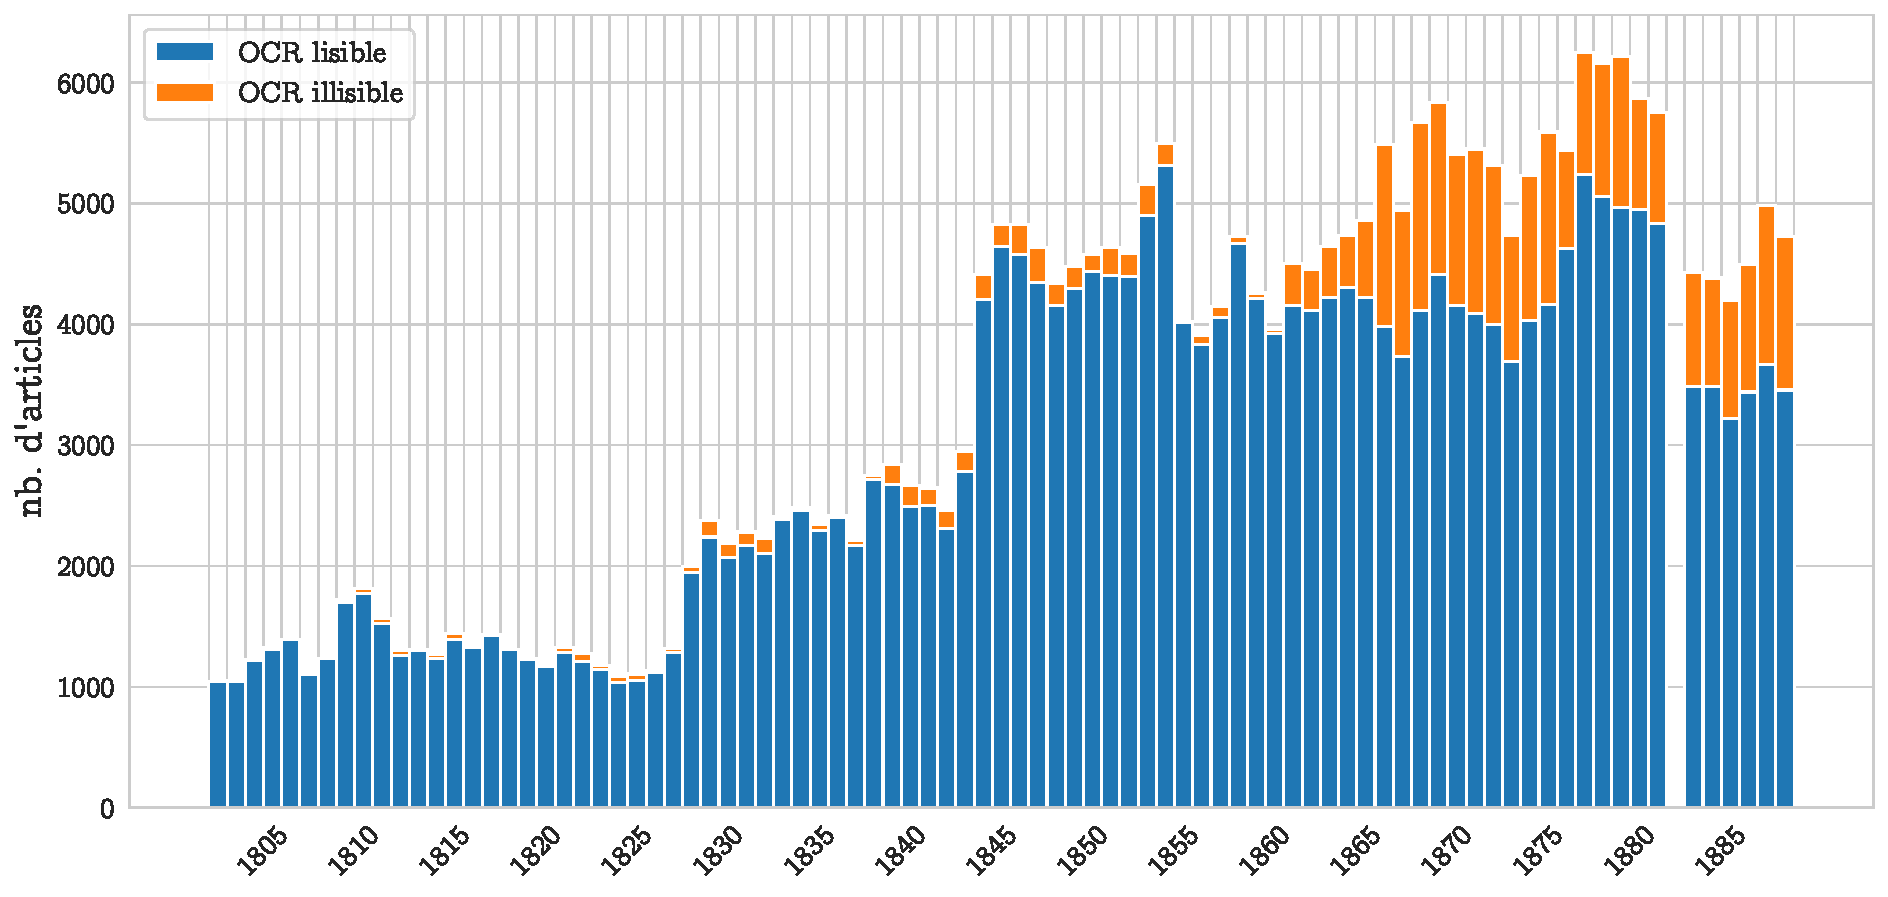
\includegraphics[width=\textwidth]{images/readability_histogram.pdf}
\caption{Distribution temporelle des données et la proportion d'articles classifiés illisibles}
\label{fig:readability_hist}
\end{figure}

En grand total, 32 709 articles, soit 11\%, du corpus entier sont considérés illisibles par le modèle SVM. Leur distribution temporelle dans le corpus, présenté sur la figure \ref{fig:readability_hist}, nous donne quelques informations sur les types d'articles qui sont normalement d'une mauvaise qualité d'OCR. La proportion de textes illisibles reste très faible jusqu'aux années 1860, d'où elle s'augmente considérablement. Mais c'est exactement là le moment où la nature du journal est en plein changement - l'on voit l'apparition de nouvelles rubriques employant des nouvelle structures de l'information. Cela sera traité dans la section suivante.

\subsubsection{Tokénisation} \label{tokenisation}

Après la classification des textes selon leur lisibilité, le contenu des articles est séparé en mots singuliers.\footnote{\texttt{./climdist/create\_sentences.py}} Cette tâche est accompli par une méthode assez simple. D'abord, les textes sont séparés par des espaces. Ensuite, chaque part est mise en minuscule et les symboles de ponctuation sont enlevés des deux côtés (cela a pour but de supprimer les virgules et les points, mais aussi les guillemets qui apparaissent souvent). Puis, chacun de ces \og mots \fg{} est évalué par une fonction qui compare la proportion de caractères réguliers dans le mot à la proportion de ponctuation, de chiffres et de caractères non latins au milieu du mot (des caractères cyrilliques sont parfois présents). La valeur maximale autorisée pour ces symboles peu courants a été fixée à 30\% pour ne pas perdre trop de l'information. Les \textit{stopwords}, i.e. les articles, les mots \og connecteurs \fg{} et les mots les plus courants dans la langue, sont également écartés. Enfin, les mots nettoyés de chaque article sont rassemblés dans une liste.\footnote{\texttt{./data/processed/RZ\_sentences.jsonl}}

L'inconvénient de cette approche est que de nombreux mots bruyants sont complètement éliminés de l'analyse. Comme les mots avec trait d'union ne sont pas pris en compte  (le saut de ligne les sépare en deux et le trait d'union est enlevé), les deux moitiés d'un même mot se retrouvent souvent comme des \textit{tokens} séparés. En revanche, lorsque, par exemple, un espace manque après un point ou une virgule, les deux mots autour du symbole de ponctuation peuvent être considérés comme des \textit{tokens} séparés. La mise en minuscules des mots réduit les détails sémantiques car en allemand, la même forme de mot peut parfois apparaître comme un nom lorsqu'elle est en majuscule, mais jouer le rôle d'un verbe ou d'un adjectif dans le cas contraire.

D'autre part, cette méthode brute est beaucoup plus contrôlable qu'une tokénisation avec un modèle de langue qui peut ne pas être reproductible et donner des résultats différents selon le contexte local. Comme le montre le chapitre suivant, les mots qui sont quelque peu altérés au cours de ce processus peuvent toujours être retrouvés dans leur forme correcte à l'aide des vecteurs de mots. La mise en minuscules peut créer une certaine ambiguïté grammaticale, mais elle permet également d'éliminer les majuscules aléatoires au milieu du mot. La perte des mots d'arrêt ne constitue pas une perte d'information pour les méthodes utilisées dans ce travail qui s'appuient fortement sur la distribution des noms, adjectifs et verbes qui ne font pas partie des plus courants du corpus. Enfin, l'utilisation de listes de \textit{tokens} rend toutes les étapes suivantes plus rapides dans le calcul.

\subsubsection{Normalisation des titres} \label{normalisation_titres}

La partie finale du prétraitement consiste à la modification des titres des articles. Une première étape utilise la distance d'édition pour converger de différentes formes orthographiques d'un même titre répandu. Avec Pandas, j'ai choisi tous les titres du corpus qui apparaissent plus de 100 fois. Ensuite, je les ai comparés aux autres titres à l'aide de la distance Levenhstein, un algorithme pour compter le nombre de modifications nécessaires pour transformer un mot (plus généralement un texte) en un autre. Par exemple, le titre \textit{Reuest« Nachrichten.} aurait besoin de 3 modifications pour être transformé en \textit{Neueste Nachrichten} (remplacer \textit{R} par \textit{N}, \textit{«} par \textit{e}, et supprimer le point).

Pour chacun de ces titres, il fallait trouver la distance maximale de Levenhstein - en surpassant cette valeur et en permettant un trop grand nombre de modifications, des formes textuelles qui ne sont pas en fait des formes erroneuses du titre en question, seront trouvés comme des faux-positifs. Par exemple, une distance de 1 permet de transformer \textit{InlaNd} en \textit{Inland} mais une distance de 2 nous mène déjà à \textit{England}).\footnote{Le processus pour trouver les distances optimales a été fait dans \texttt{./notebooks/headings.ipynb}} Pour chacun des 100 titres les plus populaires \(x_i \in \{x_1 ... x_{100}\}\), les autres titres dont la distance d'édition est inférieure ou égale à la valeur autorisée \(y_j \in \{y_1 ... y_{100} \mid \delta_j \le \Delta\}\), sont remplacés par le titre original \(x_i\). Cette opération réduit considérablement le nombre des titres uniques dans le corpus et les rend mieux analysables. Les exemples se trouvent dans le tableau (\ref{table:titles_normalised} (lignes 3, 5-7).

La deuxième type de prétraitement des titres concerne un format typique du 19\textsuperscript{e} siècle. Conformément à la structure des journaux au début de l'ère moderne, les titre de l'article reflétaient souvent la date et le lieu de provenance de l'information. Les exemples de tels titres se trouvent dans le tableau \ref{table:titles_normalised} (lignes 1-2, 4, 8-10). A l'aide d'une expression régulière (un ensemble de règles pour extraire l'information d'une chaîne de caractères), j'ai enlevé les noms des lieux et les dates et les ai placés dans des colonnes séparées du corpus : \texttt{placename} et \texttt{origin\_date}. Une telle agrégation expose l'information précieuse dans les titres et le rend plus facilement analysable dans les étapes suivantes. Plus notamment, il devient possible de regrouper les noms de lieux comparer leur fréquences (cf la section \ref{sujets_abordes}). Au total, 83 692 noms des lieux et 83 387 dates ont été détectés avec cette méthode.

\begin{table}[]
    \centering
    \small
    \begin{tabular}{lll}
\toprule
                               Titre originel &                                           Titre normalisé \\
\midrule
                   St. Petersburg, den 6. November. &                                     St. Petersburg \\
                        Lissabon, den 23. December. &                                           Lissabon \\
                                    Bekanntmachung. &                                   Bekanntmachungen \\
                          Karlskrona, den 22. März. &                                         Karlskrona \\
      Nachstellende Personen zeigen ihre Abreise... &       Nachstehende Personen zeigen ihre Abreise... \\
                 Börsen- und Handels – Nachrichten. &                    Börsen- und Handels-Nachrichten \\
            Jft zu drucken erlaubt. Im Namen de-... &                          Ist zu drucken erlaubt... \\
                          Triest, den 22. December. &                                             Triest \\
                            Vom Main, den 18. März. &                                               Main \\
                    St. Petersburg, den 16. August. &                                     St. Petersburg \\
\bottomrule
\end{tabular}
    \caption{Exemples de titres normalisés}
    \label{table:titles_normalised}
\end{table}

Après ces manipulations, une colonne pour les titres normalisés a été ajouté au corpus (\texttt{heading2}). Dans cette colonne se trouvent les formes normalisés avec l'expression régulière et les noms des lieux, si applicable. Au grand total, 102 378 titres ont été modifiés ou normalisés. L'effet devient évident en comparant les nombres des titres les plus fréquentes avant et après la normalisation (figure \ref{fig:title_normalisation}). Grâce à la convergence des différentes formes mal-océrisées et à la détection des toponymes, la variance des titres s'est réduite considérablement. Cela montrera son utilité dans la section suivante.

\begin{figure}[h]
\centering
\captionsetup{justification=centering}
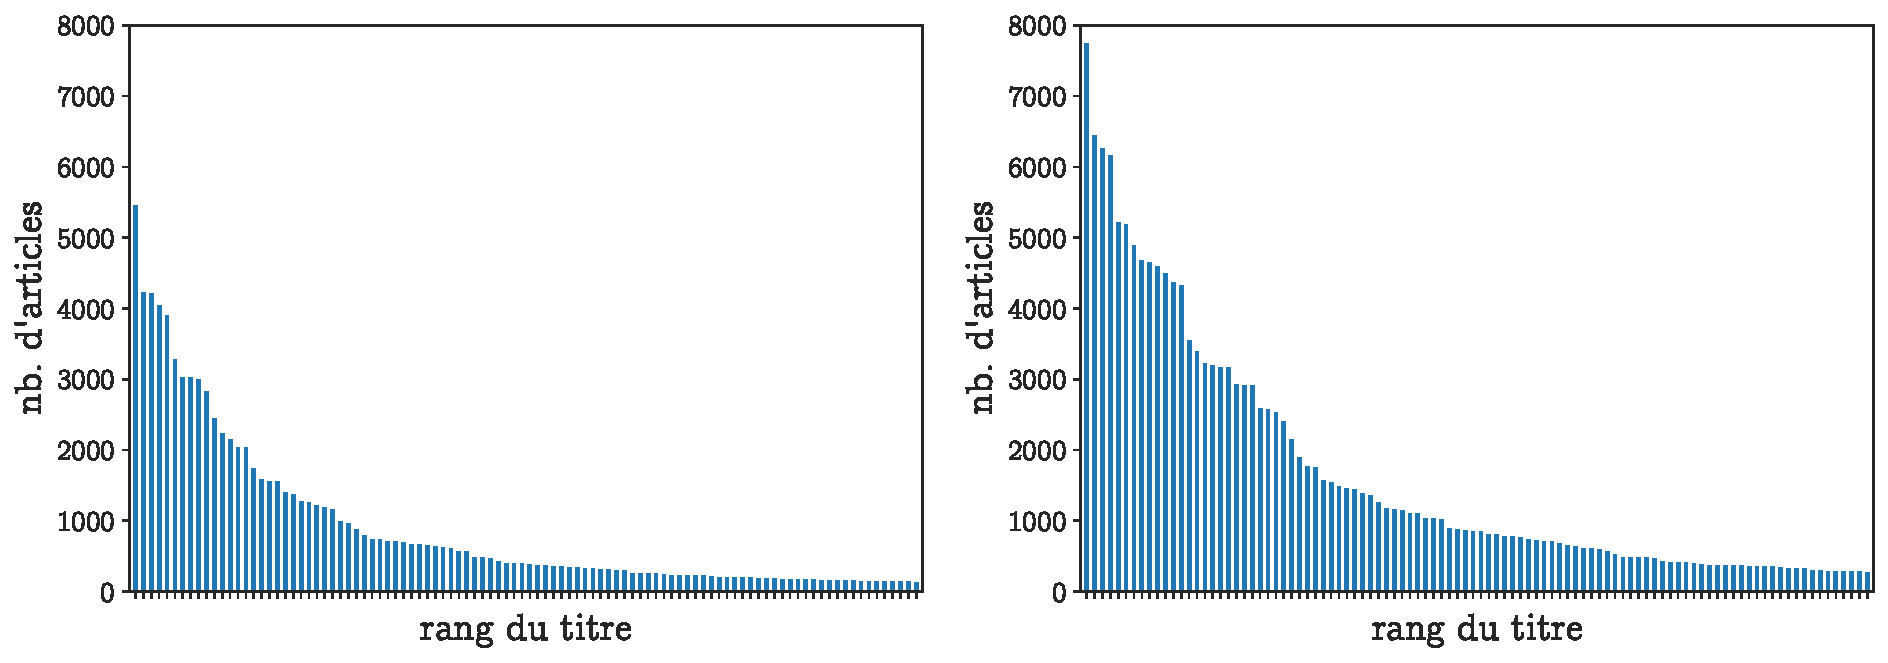
\includegraphics[width=\textwidth]{images/title_normalisation.pdf}
\caption{La fréquence des 100 titres les plus courants avant la normalisation (à gauche) et après}
\label{fig:title_normalisation}
\end{figure}




\subsection{Exploration du corpus\footnote{Les manipulations contenues dans cette section se trouvent dans le notebook :\\ \texttt{./notebooks/corpus\_exploration.ipynb}}} \label{exploration}

\subsubsection{Tendances de la quantité et la répartition de l'information} \label{corpus_tendencies}

%Cette section présente un aperçu général du corpus et ses tendances quantitatives, mais jette également un regard sur le contenu des articles et démontre les sujets principaux abordés au cours du siècle.

L'information n'est pas répartie de façon homogène. Au cours de 86 ans\footnote{cf. la note en bas de la page \pageref{86_years}}, il y a des changements par rapport à la fréquence de parution, ainsi bien que une tendance à l'allongement des articles et l'augmentation de la masse d'information. Ces évolutions sont présentées sur la figure \ref{fig:text_mass}. Tout d'abord, l'on remarque que la fréquence de parution est divisée en trois étapes (en haut à gauche de la figure). Dans la première étape, avant 1830, \textit{Rigasche Zeitung} était publié ca. 100 fois par an, soit chaque mercredi et samedi. En 1828-1829, les jours de publication étaient le mardi, le jeudi et le samedi. Enfin, à partir de la fin de 1843, \textit{Rigasche Zeitung} est devenu un quotidien publié 6 fois par semaine, soit tous les jours sauf le dimanche. En haut à droite de la figure, le nombre moyen d'articles inclus dans un numéro est présenté. L'on y voit une croissance générale qui est pourtant interrompue par des périodes de recul ou les numéros ont contenu moins d'articles en moyenne.

Le graphique en bas de la figure \ref{fig:text_mass} décrit la longueur textuelle des numéros (en nombre de caractères). Pour chaque décennie, une \og boite à moustaches \fg{} est présentée. Dans chaque boîte, la ligne orange marque la médiane pour la décennie donnée - cela signifie qu'une moitié des articles ont une longueur supérieure à cette valeur. Le bord supérieur de la boîte marque la longueur qui est supérieur à celle de 75\% des données. De la même manière, 25\% des textes sont plus courtes au bord inférieur de la boîte. Les petites lignes horizontales marquent les minima et maxima des données pour la décennie. Les points qui restent au-delà de ces lignes sont les valeurs aberrantes, c'est-à-dire les articles exceptionnellement courts ou longs dans le contexte de la décennie.

\begin{figure}[h]
\centering
\captionsetup{justification=centering}
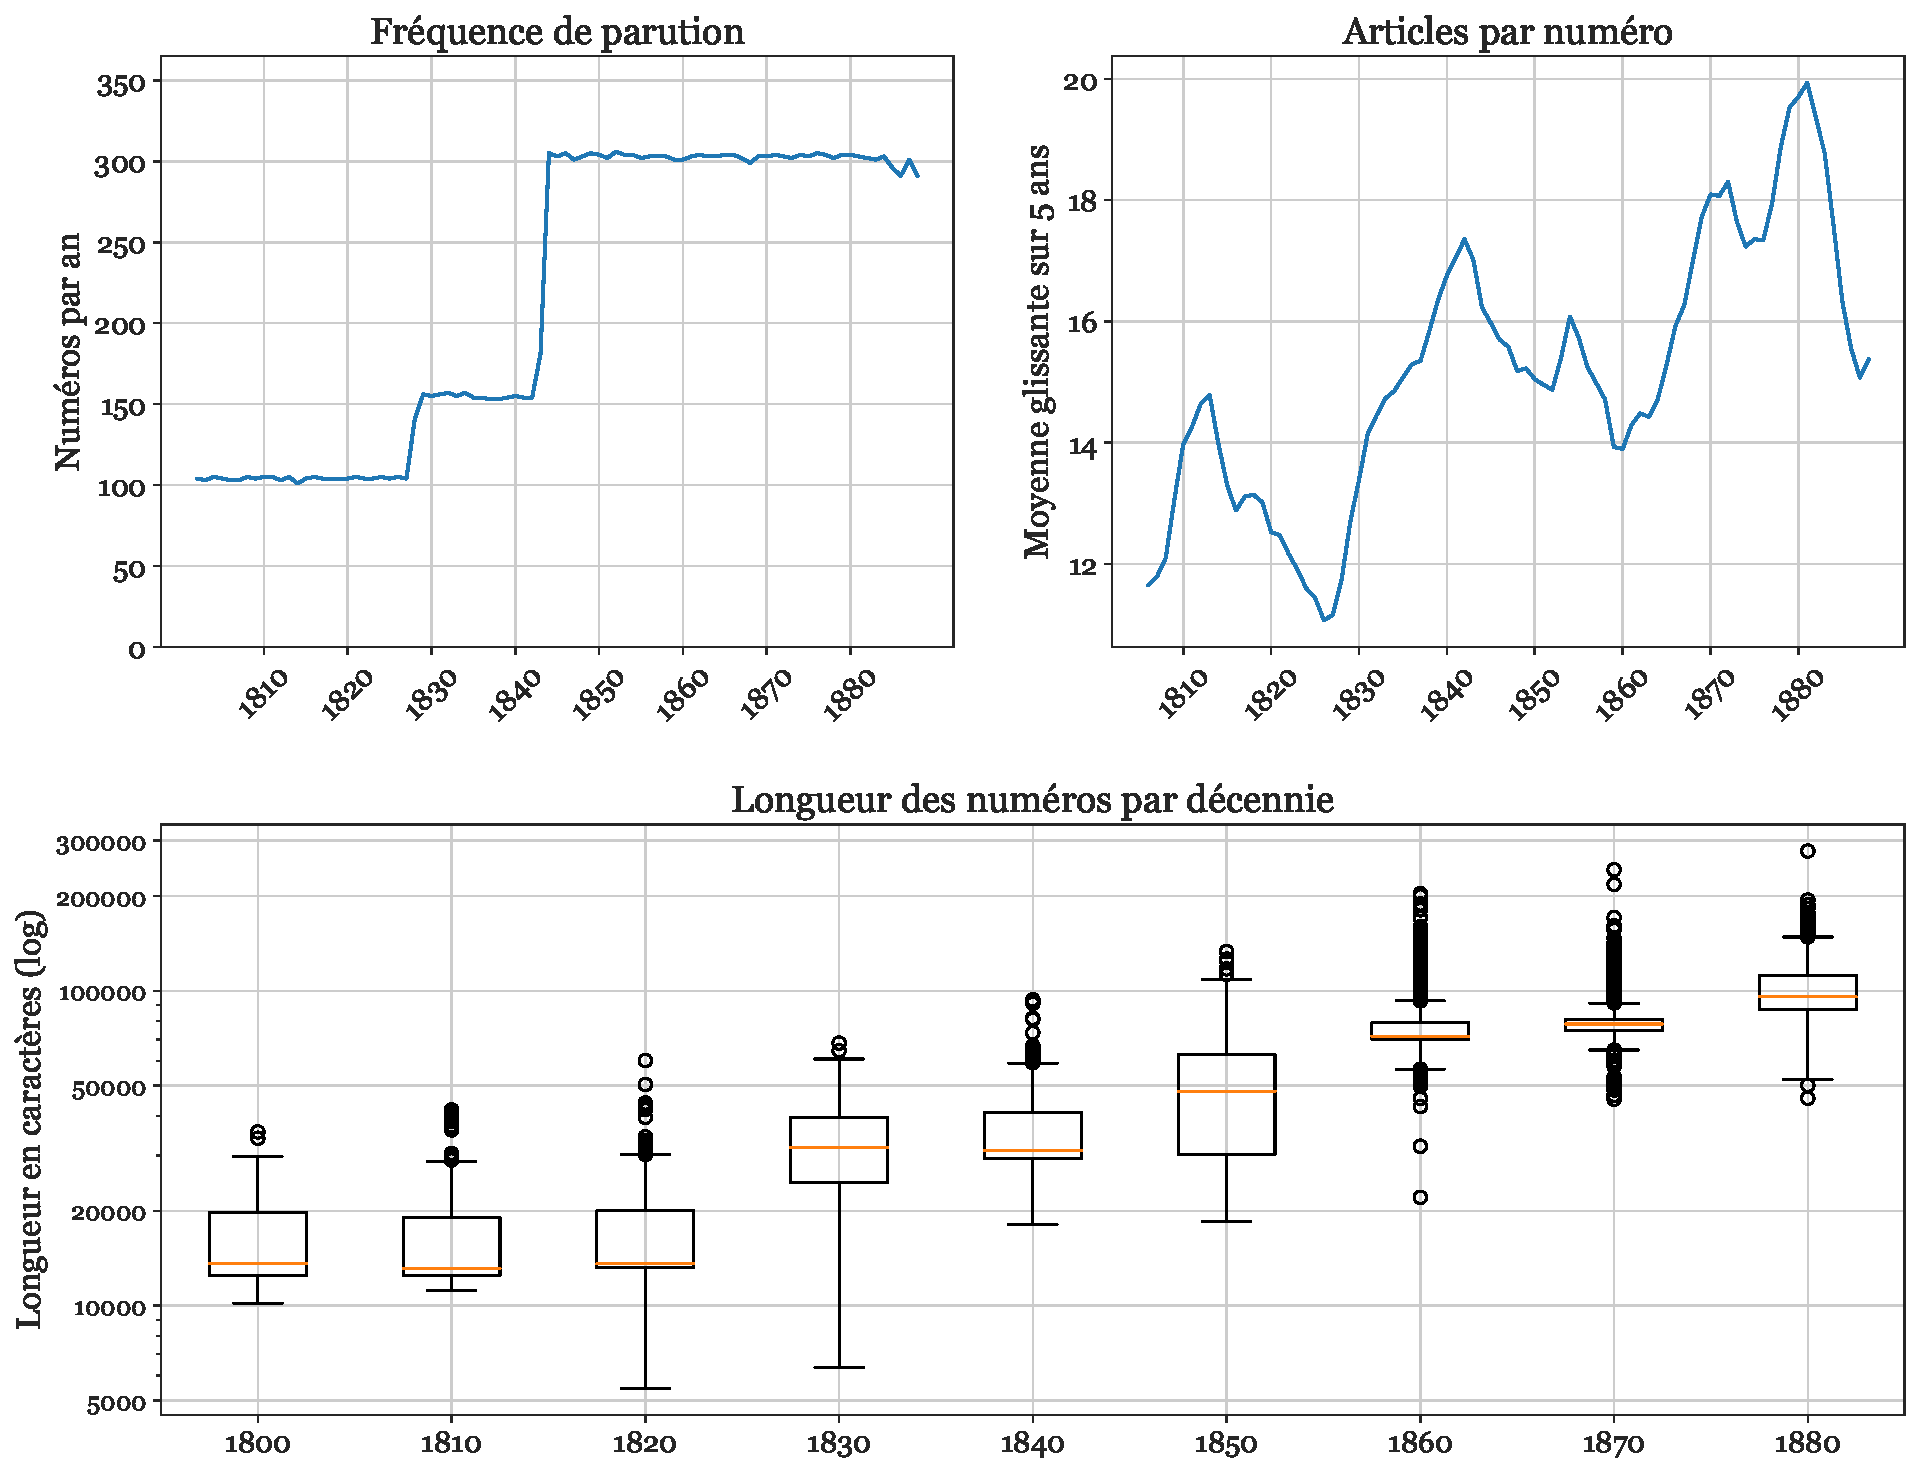
\includegraphics[width=\textwidth]{images/text_mass.pdf}
\caption{Evolutions par rapport à la quantité et la répartition temporelle de l'information}
\label{fig:text_mass}
\end{figure}

A l'aide des boîtes à moustaches, l'on perçoit que les numéros ont été devenus plus longs au cours de la siècle. Jusqu'aux années 1830, le nombre de caractères dans un numéro restait normalement entre 10 000 et 30 000 (le minimum passant à 5000 dans les années 1820). Dans les années 1830-1850, la plupart des numéros étaient plus longs qu'auparavant, la médiane s'élevant à 50 000 caractères en 1850-1859. Les trois dernières décennies voient une configuration différente : les numéros deviennent plus longs avec une médiane finale de ca. 100 000 caractères en 1880-1888, mais il y a un nombre beaucoup plus élevé de valeurs aberrantes.\footnote{Il faut noter que l'axe vertical du graphique est sur une échelle logarithmique, ce qui donne une fausse impression que la distribution de la longueur des numéros est devenue plus étroite.}

En regardant les numéros avec une longueur disproportionnée, il dévient évident qu'à partir des années 1860, des annexes et des suppléments étaient souvent publiés en pièce jointe du numéro. La nature de ces types de textes était variée - des longues listes officielles des promotions des fonctionnaires à collections d'histoires littéraires, en passant par les informations sur les affaires judiciaires. La plupart du temps, le contenu de ces suppléments n'est pas strictement journalistique, mais ils ont quand même été numérisés par LNB comme parties des journaux, parfois portant leur longueur jusqu'à 40-50 pages.


\subsubsection{Contenu} \label{sujets_abordes}

Le journal change également dans le sens de son contenu. Ces dynamiques peuvent être perçues par les titres des articles et leur évolution dans le temps. Le tableau \ref{tab:common_headings} présente les 30 titres les plus fréquents dans le corpus entier, qui comptent pour ca. 40\% de tous les textes.\footnote{Les 10 titres les plus fréquents comptent pour 20\% et les 100 titres les plus fréquents pour 57\% du corpus}. L'on voit que ces titres se répartissent en quelques catégories principales. Très fréquents sont les articles portant le nom de l'origine de ses contenus.\footnote{cf. la section \ref{pretraitement} pour les modifications qui facilitent le traitement des toponymes dans les titres}. Les plus populaires parmi eux sont Paris, Londres, Vienne, Berlin, la France, l'Allemagne, St. Petersbourg, etc. - autrement dit les centres du pouvoir économique et politique dans l'Europe du XIX\textsuperscript{e} siècle qui canalisaient une grande proportion des informations importantes pour les lecteurs à Riga. Le public s'intéressait aux développements publics dans les grandes capitales (surtout en temps de guerre), ainsi qu'aux actualités coloniales qui se concentraient dans les métropoles. Les marchands suivaient des développements commerciaux qui avaient un effet sur leur métier. Le seconde type d'articles et celui des informations récurrents, p. ex. des listes d'étrangers arrivés ou départis par voie maritime ou terrestre, des télégrammes, les horaires de trains ou des rapport systématiques sur les commerce et la bourse.

\begin{table}[h]
    \centering
    \small
    \begin{tabular}{llr}
\toprule
                 \textbf{Titre} &         \textbf{Traduction française} & \textbf{Nb.} \\
\midrule
                          Paris &                                 Paris &      7771 \\
            Neueste Nachrichten &                   Dernières nouvelles &      6473 \\
                           Riga &                                  Riga &      6287 \\
                         London &                                Londres &      6192 \\
Witterungsbeobachtungen in Riga &   Observations météorologiques à Riga &      5242 \\
                           Wien &                                Vienne &      5216 \\
               Bekanntmachungen &                              Annonces &      4911 \\
                         Berlin &                                Berlin &      4684 \\
                     Frankreich &                                France &      4616 \\
             Angekommene Fremde &                     Etrangers arrivés &      4527 \\
        Inländische Nachrichten &                 Nouvelles domestiques &      4388 \\
                    Deutschland &                             Allemagne &      4350 \\
                 St. Petersburg &                       St. Petersbourg &      3642 \\
                     Telegramme &                           Télégrammes &      3571 \\
                         Inland &                [Affaires] domestiques &      3426 \\
                        Italien &                                Italie &      3246 \\
                         Inhalt &                   Contenu [du numéro] &      3217 \\
                    Vermischtes &                   [Actualités] mixtes &      3195 \\
     Groszbritannien und Irland &            Grande-Bretagne et Irlande &      3190 \\
         Tägliche Eisenbahnzüge &                     Trains quotidiens &      2958 \\
                         Madrid &                                Madrid &      2945 \\
                        Locales &                     [Affaires] locaux &      2939 \\
      Ist zu drucken erlaubt... &                Autorisé à imprimer... &      2621 \\
                    Oesterreich &                              Autriche &      2603 \\
                Deutsches Reich &                       Empire allemand &      2560 \\
Börsen- und Handels-Nachrichten & Actualités boursières et commerciales &      2435 \\
                 Konstantinopel &                        Constantinople &      2171 \\
                        Brüssel &                             Bruxelles &      1928 \\
                        England &                            Angleterre &      1802 \\
   Telegraphische Coursberichte &      Rapports de cours télégraphiques &      1788 \\
\bottomrule
\end{tabular}
    \caption{Les titres les plus courants dans le corpus}
    \label{tab:common_headings}
\end{table}

Bien entendu, ces catégories ne restent pas inchangées dans le temps. La partie suivante explore les développements principaux sur le contenu des journaux à l'aide des titres. Les titres ne reflètent pas complètement le contenu de l'article et ils ne sont pas toujours exacts (à cause d'une mauvaise segmentation, par exemple), mais ils sont pourtant adaptés pour donner une vue global des sujets traités dans le journal.

Dans un premier temps, l'on peut regarder les lieux de provenance de l'information. La figure \ref{fig:headings_places} présente la part de l'importance des 10 noms de lieux étrangers les plus répandus dans le tableau \ref{tab:common_headings}, ainsi que les titres \textit{Inland}, \textit{Inländische Nachrichten}, \textit{Locales} et \textit{Riga}. Cette figure présente les titres de manière relative, ce qui signifie que la hauteur du graphique n'indique pas une valeur absolue, mais plutôt le pourcentage de tous les articles d'une année donnée.

\begin{figure}[h]
\centering
\captionsetup{justification=centering}
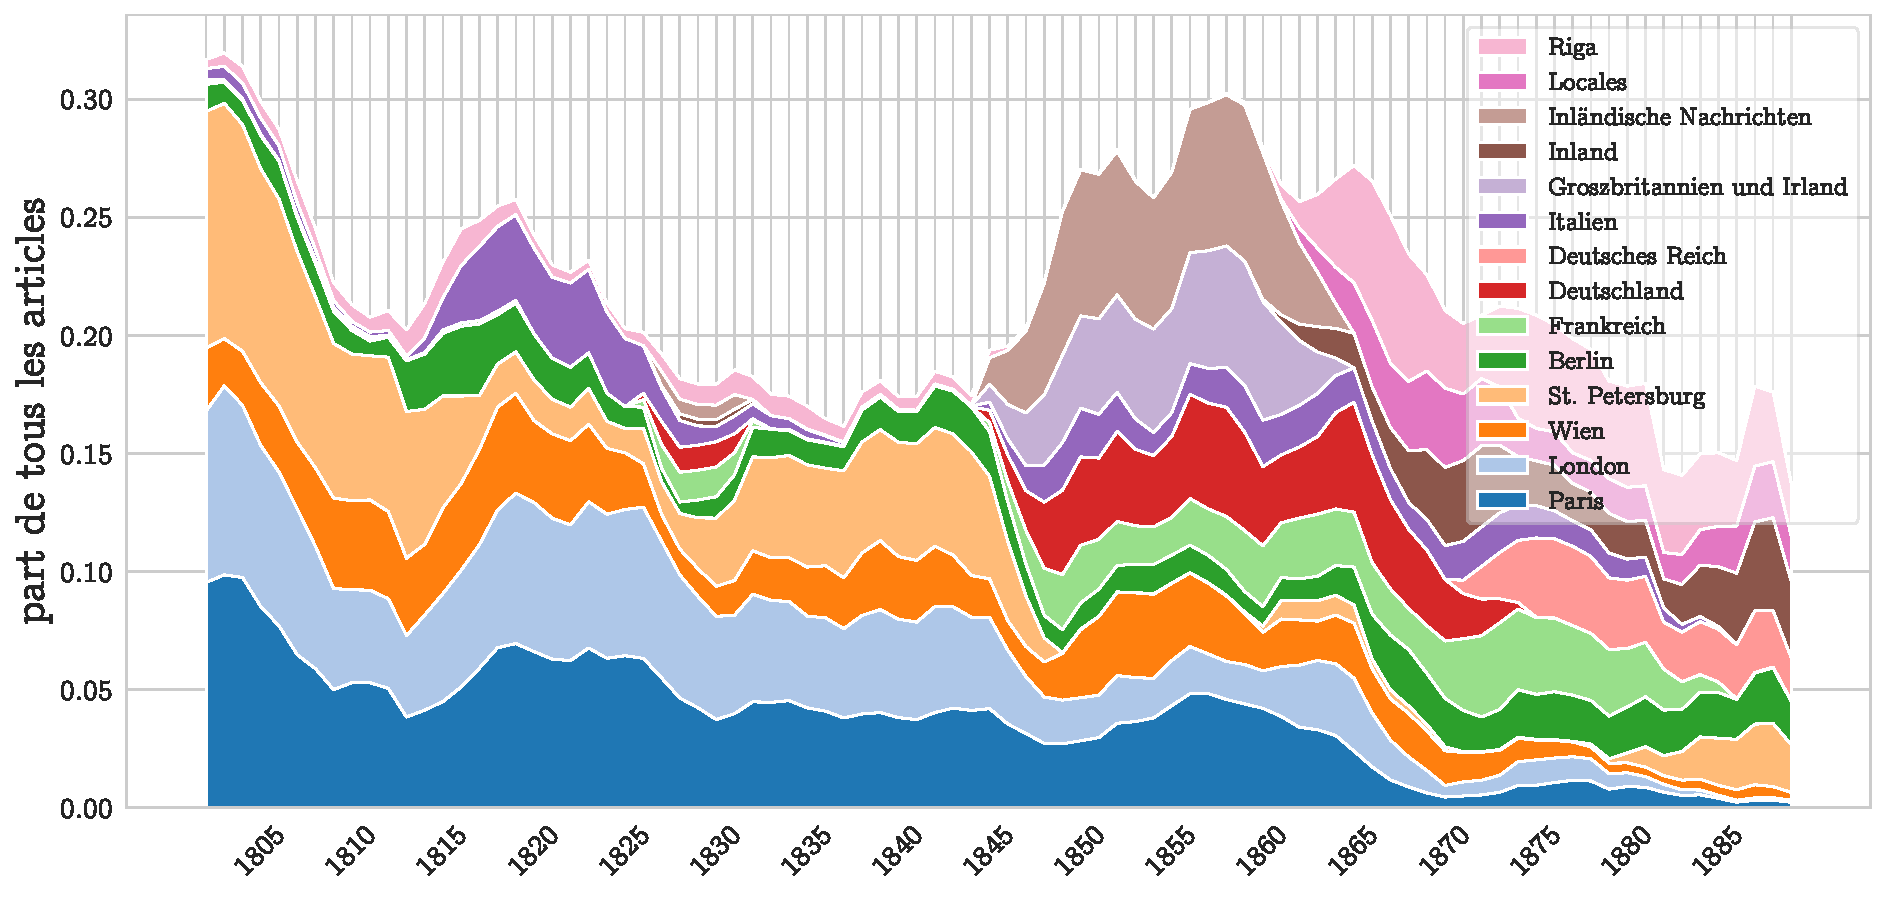
\includegraphics[width=\textwidth]{images/headings_places.pdf}
\caption{Importance relative des noms de lieux principaux dans les titres d'articles}
\label{fig:headings_places}
\end{figure}

L'on constate qu'au début de la période observée, les trois villes les plus importants paraissaient dans presque un tiers des titres, pendant que leur importance est tombée à moins de 5\% en 1888. D'une part, les titres ne reflètent pas toujours fidèlement le contenu des articles - les changements dans la structure des journaux, les décisions prises par LNB au stade de la segmentation, ainsi que un certain nombre des titres qui n'ont pas été capturés par l'expression régulière, influencent les proportions observées sur le graphique. Au fil du temps, différentes nouvelles de villes étrangères pourraient, par exemple, être progressivement incluses dans des articles aux noms plus généraux, déplaçant ainsi les noms de lieux au sein de l'article.

D'autre part, ces tendances reflètent probablement des vraies évolutions par rapport au contenu du journal. Au fur et à mesure que le réseau de journaux s'imbrique au cours du siècle et que la vitesse de l'information augmente, les journaux s'adaptent aux changements. Il est clair que le nombre de sources disponibles et accessibles était beaucoup plus petit au début du siècle qu'à la fin. La nature de ce que l'on considérait \og médiatique \fg{} a également changé. Dans les premières décennies du XIX\textsuperscript{e} siècle, les nouvelles dignes d'intérêt concernent des événements survenus à l'étranger, s'inscrivant ainsi dans la logique de la presse des débuts de l'ère moderne. Les informations locales étaient principalement transmises par d'autres moyens (par le bouche à oreille, affiches, etc.). Toutefois, au milieu du siècle, on constate un changement de cette tendance. Des nouvelles catégories importantes, d'abord \textit{Inland}/\textit{Inländische Nachrichten}, ensuite \textit{Locales} et \textit{Riga}, apparaissent. Cela représente un \og retour sur soi \fg{} très intéressant qui apparaît également dans d'autres journaux locaux de l'époque.\footnote{De 1836 à 1863, le journal \textit{Inland} était publié à Tartu (\textit{Dorpat}). Ce journal a été le premier dans les gouvernements Baltes à s'éloigner de la vision des nouvelles comme quelque chose qui vient toujours de l'étranger. Il est possible que l'apparition de \textit{Inländische Nachrichten} dans le \textit{Rigasche Zeitung} dans le même temps est une réponse à cela.} Dans \textit{Rigasche Zeitung}, la catégorie \textit{Inland} représente en fait l'ensemble de l'empire russe avec un accent sur les villes des gouvernements Baltes et apparaît au même temps que la fréquence de parution atteint 6 jours par semaine. La catégorie \textit{Locales} se concentre principalement sur les événements au niveau de Riga ou ses alentours.

Une autre évolution très intéressante, ou plutôt une rupture, peut être observée lorsque nous examinons les titres du tableau \ref{tab:common_headings} qui expriment quelque chose sur la forme ou le mouvement de l'information. En regardant les titres sélectionnés pour la figure \ref{fig:headings_other}, l'on remarque tout de suite la rupture vers l'année 1860. En fait, ce graphique, ainsi que le précédent, a été crée avec une moyenne glissante sur 5 ans pour niveler un peu les tendances et pour les rendre plus faciles à percevoir. En retirant la moyenne glissante, cette rupture est encore beaucoup plus subite - tous les titres concernés tombent à zéro en 1855 et ne remontent qu'en 1861. Cela correspond à peu près à la période de la guerre de Crimée (1853-1856), pendant laquelle les ports russes étaient bloqués par les marines de la France et le Royaume-Uni. En situation de guerre, la presse avait sa propre sorte de \og silence radio \fg{}, au moins en ce qui concerne ces importantes catégories d'articles, car la masse totale d'articles et de l'information n'est pas considérablement influencée.

\begin{figure}[h]
\centering
\captionsetup{justification=centering}
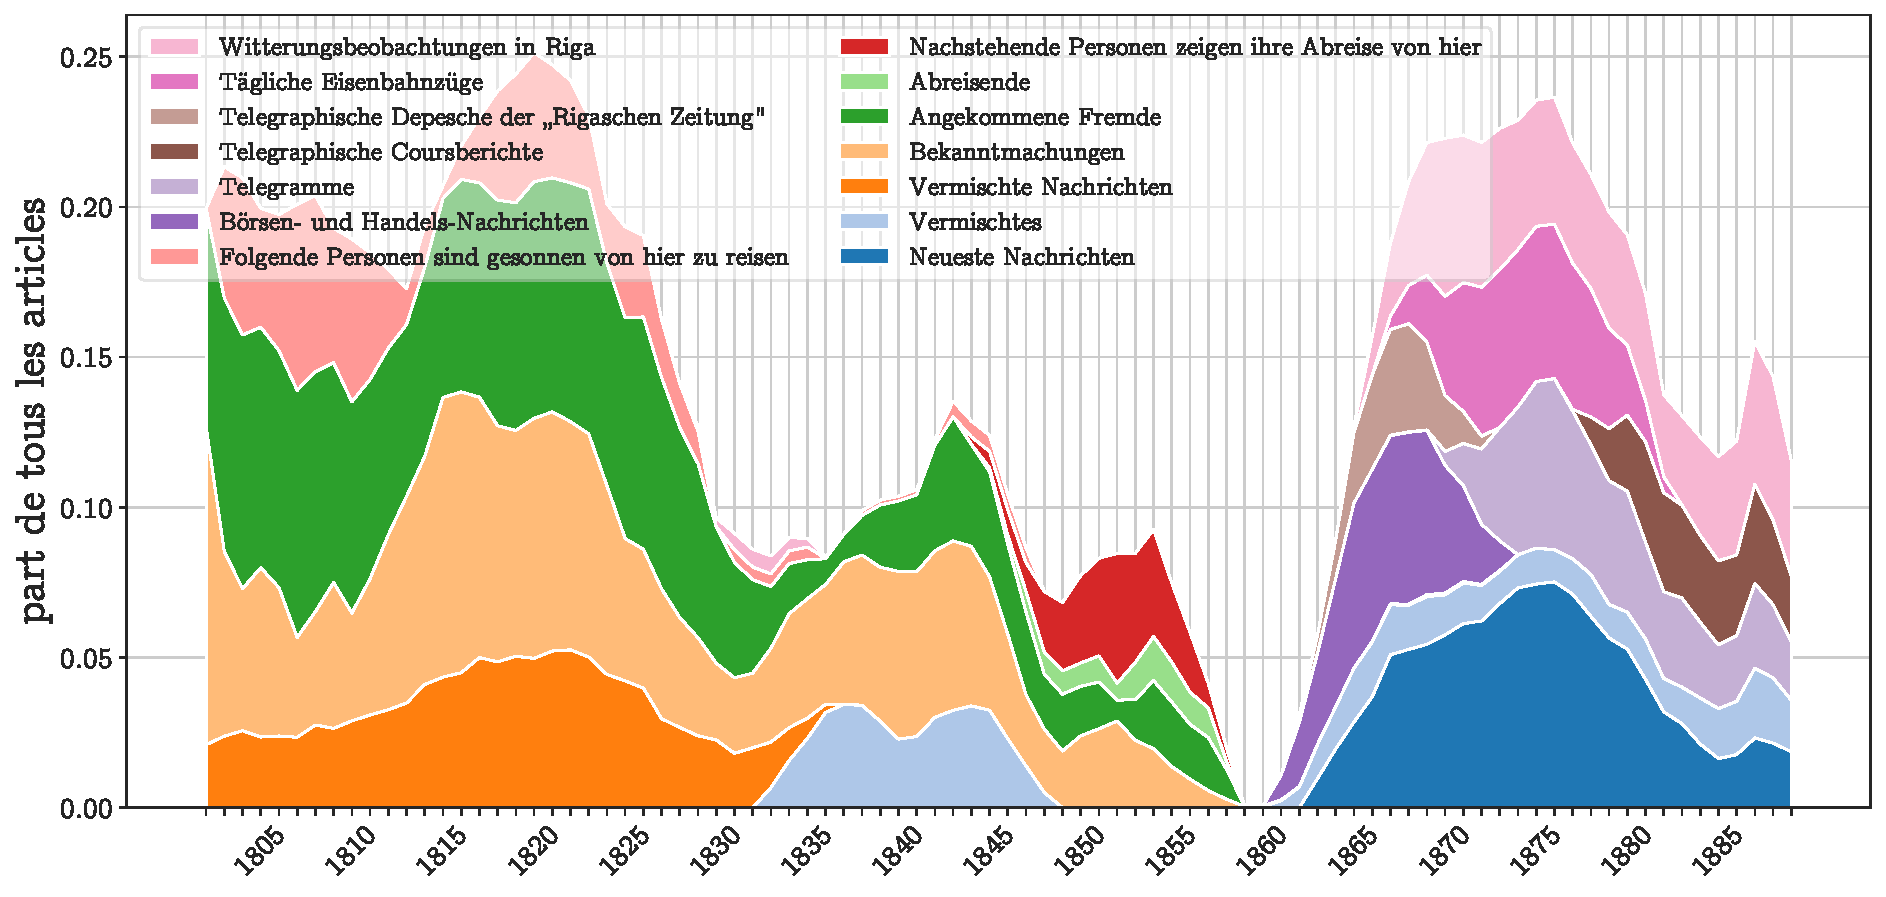
\includegraphics[width=\textwidth]{images/headings_other.pdf}
\caption{Importance relative des titres donnés}
\label{fig:headings_other}
\end{figure}

Les années 1855-1860 marquent un changement brusque pour la \textit{Rigasche Zeitung} surtout car le journal qui a émergé après cette période était très différent de celui qui l'avait précédé. Les vieilles catégories d'information qui étaient importantes auparavant, notamment les étrangers arrivés, les partances et les annonces, disparaissent complètement. A leur place, une multitude de rubriques inédites font surface : télégrammes. actualités boursières, horaires des trains etc. Prises ensemble, ces nouvelles catégories d'information qui ont rapidement constitué une part considérable du numéro moyen, peuvent être considérées collectivement comme un signe de l'avènement de la modernité. En novembre 1852, l'un des premières lignes télégraphiques publiques en Europe du Nord a été ouverte entre Riga et Bolderāja (\textit{Bolderaa}), où le fleuve Daugava (\textit{Düna}) atteint la mer Baltique, environ 10 km du centre de Riga. Le télégraphe fût y installé principalement pour avertir les marchands de Riga sur les conditions météorologiques et maritimes en temps réel, ce qui était considéré comme crucial pour la navigation.\footnote{\og Comme il est probable que la communication avec la Bolderaa sera bientôt et peut-être déjà fermée, nous n'en apprendrons naturellement rien, sinon ce que les personnes qui montent dans nos clochers, souvent armées de jumelles, jugeront bon de nous communiquer. C'est pourquoi nous ne pouvons pas assez répéter le souhait que des dispositions soient prises pour que nous soyons sûrs et rapides soient informées de ce qui s'y passe et de l'intérêt qu'elles suscitent. un intérêt si général. \fg{} \textit{Inland}, 20.04.1836} En septembre 1861, Riga a eu sa première liaison ferroviaire avec la ville de Daugavpils, qui était à son tour reliée à Saint-Pétersbourg, Vilnius et Varsovie.\footnote{J'ai encore besoin d'un référence ici et je vais détailler ce passage un peu - p. ex. quand exactement Riga a été relié à St. Pétersbourg par le télégraphe}

Ces développements sont bien reflétés dans la structure de \textit{Rigasche Zeitung} à partir des années 1860. L'on voit la disparition complète de la rubrique des passagers arrivés - autrefois une source principale pour toute personne qui voulait recevoir des nouvelles directes des provinces de l'empire ou d'autres villes d'Europe. L'avènement des nouvelles voies de communication a rendu caduque les anciens modes de pensée et a inséré le journal dans un réseau moderne d'information en expansion constante, constitué de chemins de fer, de lignes télégraphiques et, au XX\textsuperscript{e} siècle, de téléphones. Les informations sur les cours de la bourse dans des villes éloignées pouvaient être communiquées en quelques minutes et les trains ont érodé l'attrait du voyageur lointain. Au lieu de regrouper les nouvelles redondantes ou moins importantes sous la rubrique \og nouvelles mixtes \fg{} (\textit{Vermischtes}), le journal a commencé à les présenter comme les \og dernières nouvelles \fg{} - ici aussi, la rapidité et la fraîcheur ont de la valeur.

Il faut aussi s'arrêter sur la rubrique des observations météorologiques qui sont parmi les catégories de nouvelles les plus nombreuses. Un peu à l'inverse de ce à quoi le lecteur moderne est habitué, il ne s'agissait pas de prédictions météorologiques, mais de rapports sur le temps du ou des jours précédents. Avec quelques changements au fil du temps, ils se composaient normalement de quelques mots-clés (exprimant les précipitations et la vitesse du vent) et de mesures numériques (sur la température et la pression atmosphérique) disposés dans une sorte de tableau. Malheureusement, c'est ce type de présentation qui rend les observations météorologiques inutilisables dans le contexte du présent travail, car l'OCR est souvent de très mauvaise qualité sur ces articles (voir le tableau \ref{tab:readability_example} pour un exemple). Seuls 45 (!) des 5194 articles de cette catégorie ont été considérés comme lisibles par le modèle SVM. Les exclure des prochaines étapes de l'analyse signifie beaucoup de potentiel inutilisé, mais aussi un objectif plus clair - ils diffèrent très clairement du type descriptif d'informations météorologiques que l'on trouve normalement dans d'autres types d'articles. Les observations météorologiques peuvent encore témoigner de l'intérêt croissant pour le temps et d'une approche empirique renouvelée dans les dernières décennies du siècle, ce qui peut également être utile pour comprendre les textes de type narratif.


\clearpage

\section{Vecteurs et mots-cleś (placeholder)} \label{vecteurs_etc}

Ce chapitre prend en vue le contenu \og climatique \fg{} au niveau des mots isolés qui signifient des phénomènes météorologiques en allemand et leur présence dans le corpus. Le corpus sera tout d'abord vectorisé. Ensuite, un vocabulaire fixe des mots \og météorologiques \fg{} sera construit. Les apparitions de chaque mot-clé seront comptées afin de voir leur distribution et d'effectuer des analyses comparatives ainsi que temporelles. La vectorisation des textes offre également la possibilité de visualiser les relations et les tensions sémantiques entre les mots. Enfin, les contextes immédiats des mots-clés sera étudié. Les analyses de ce chapitre restent au niveau des mots individuels et leurs contextes proches, mais peuvent être mises dans le contexte des tendances générales exposées dans le chapitre précédent et forment une base pour les analyse de sujets dans la partie suivante.

La partie actuelle du travail part de la notion simple que les textes dans le corpus qui contiennent de l'information sur le climat et le temps sont reconnaissables par la présence de certains mots-clés. Le défi principal de cette approche se présente sous la forme du bruit dans le corpus : une liste des mots pertinents ne compterait jamais toutes les formes orthographiques qui apparaissent dans l'intégralité d'articles. Une prémière tentative de contourner ce problème de variance textuelle a été faite avec les méthodes de la reconnaissance d'entités nommées (NER). Selon D. Jurafsky et J. Martin, 

\begin{displayquote} Une entité nommée est en gros, tout ce qui peut être désigné par un nom propre : une personne, un lieu, une organisation. La tâche de la reconnaissance des entités nommées (NER) consiste à trouver des parties de texte qui constituent des noms propres et à marquer le type d'entité. Quatre balises d'entité sont les plus courantes : PER (personne), LOC (lieu), ORG (organisation) ou GPE (entité géopolitique). Cependant, le terme entité nommée est généralement étendu pour inclure des choses qui ne sont pas des entités en soi, notamment des dates, des heures et d'autres types d'expressions temporelles, et même des expressions numériques comme les prix. \footnote{Jurafsky, Martin, p. 153} \end{displayquote}

\label{NER_model}
L'idée d'une approche des descriptions climatiques et météorologiques via des entités nommées reposait donc sur le fait de considérer tous les mots-clés pertinents comme appartenant à une catégorie distincte d'entités qui peuvent ensuite être détectées par un modèle de langage. Comme un tel modèle ne repose pas sur une liste fixe des formes orthographiques mais prend en compte un nombre des paramètres cachées dans le contexte, il pourrait théoriquement détecter des mots non vus précédemment. Un modèle supervisé de la reconnaissance des entités nommées a donc été entraîné : toutes les entités dans une échantillon ont été annotées manuellement pour apprendre l'ordinateur à reproduire cette logique sur le reste du corpus. L'échantillon comprenait 400 textes et a été annotée avec la schéma suivante :

\vspace{1ex}
\begin{itemize}[label=$\bullet$]
    \item \texttt{WEA} - phénomènes météorologiques exprimées par des substantifs ou des groupes nominaux, ainsi que quelques mots plus généraux liés au climat (853 instances dans l'échantillon) 
    \item \texttt{LOC} - lieux (2939 instances)
    \item \texttt{DAT} - dates (1035 instances)
    \item \texttt{PER} - noms de personnes (1320 instances)
\end{itemize}
\vspace{2ex}

La schéma reflète aussi les buts initiaux de la recherche qui visaient une détection, datation et géolocalisation des événements climatiques. En se basant sur la structuration d'information dans le journal, l'hypothèse était que l'occurrence d'un mot clé est souvent accompagnée par une date et le lieu. La quatrième catégorie, \texttt{PER}, était ajoutée à la schéma pour éviter la confusion entre les toponymes et les noms de personnes (p. ex. les noms des nobles sont souvent les lieux de leur provenance), ainsi qu'entre les phénomènes climatiques et les noms de personnes (certains mots comme \textit{Sturm} apparaissent parfois comme des noms de famille en allemand).

Toutefois, la performance du modèle de reconnaissance des entités nommés formé sur ces données était trop faible pour effectuer des analyses significatives. La précision (combien des occurrences trouvées sont correctes), ainsi que le rappel (combien des occurrences totales ont été détectés) étaient médiocres, un fait lié surtout au bruit introduit au stade de l'océrisation, mais aussi aux particularités d'un texte historique qui peuvent confondre un modèle dont le fond a été créé sur des données contemporaines. La prémisse théorique de considérer les événements climatiques comme des entités nommées peut également avoir ses limites car strictement, il ne s'agit des noms propres.

Ces circonstances n'offraient pas trop de choix pour une amélioration du modèle. Une possibilité aurait été d'adapter le modèle de langue au corpus et à la langue historique qui, à son tour, aurait nécessité un travail très ardu et technique, sans garantir de meilleurs résultats. La deuxième option, la plus évidente, aurait été l'augmentation des données d'entraînement. Cela, toutefois, ne montraient pas de signes prometteurs d'amélioration, p. ex. entre des échantillons de 300 et de 400 textes. Le temps nécessaire pour l'annotation et le double contrôle aurait était si long qu'il paraissait mieux de s'appuyer sur une simple distribution des mots.


\subsection{Vecteurisation du corpus} \label{entity_ruler}

L'échec d'une approche supervisée m'a amené à une approche par un vocabulaire fixe. Afin de contourner le problème du bruit décrit ci-dessus, j'ai opté pour une solution qui s'appuie sur la similarité vectorielle entre les formes \og propres \fg{} et les formes alternatives. L'idée de la sémantique vectorielle repose sur l'hypothèse de distribution développée dans les années 1950. Selon celle-ci, le plus que les significations d'un mot et l'autre sont similaires, le plus ils apparaissent dans un contexte similaire. Par exemple, les mots voisins de \textit{voiture} et \textit{automobile} sont très similaires. L'hypothèse de distribution dit alors que leurs significations devront être très similaires ou presque identiques, car ils sont interchangeables dans la plupart des cas.\footnote{Jurafsky, Martin, p. 96.} Donc, \og l'idée de la sémantique vectorielle est de représenter un mot comme un point dans un espace sémantique multidimensionnel qui est dérivé ... des distributions des mots voisins \fg{}.\footnote{Jurafsky, Martin, p. 100.}

Il existent plusieurs méthodes pour calculer les vecteurs des mots (i.e. les coordonnées qui définissent leur positionnement dans l'espace multidimensionnel). Dans le travail actuel, la méthode \textit{word2vec} est utilisée. Publiée par Tomas Mikolov et ses collègues en 2013,\footnote{Mikolov 2013 réferences} \textit{word2vec} utilise la distribution des mots dans un corpus pour entraîner un classificateur pour la tâche \og est-il probable que le mot \textit{x} apparaisse près du mot \textit{y} ? \fg{}. Dans le cas de \textit{word2vec}, les prédictions elles-mêmes n'ont pas réellement de valeur. A leur place, les pondérations (\textit{weights}) du classificateur sont utilisées comme les vecteurs.\footnote{Les pondérations sont les paramètres que le modèle apprend à ajuster au cours de l'entraînement. Dans un réseaux de neurones, les pondérations sont en fait les multiplicateurs qui modifient les valeurs d'entrée à chaque couche du réseaux.} Cela veut dire que les chiffres ne sont pas d'une interprétation directe, mais ils définissent quand même la position des mots dans l'espace sémantique - ils ont une valeur relative. Une fois que les vecteurs sont calculées, des simples opérations mathématiques peuvent être appliquées pour calculer la distance entre eux, ce qui correspond à une similarité dans la signification selon l'hypothèse de distribution.\footnote{Jurafsky, Martin, p. 112-113.}

Pour calculer les vecteurs des mots du corpus LNB, les articles \textit{tokenisés}\footnote{\texttt{.data/processed/RZ\_sentences.jsonl}} ont été parcourus par le modèle \textit{word2vec}.\footnote{\texttt{./climdist/train\_word2vec.py} - les paramètres pour l'entraînement étaient \texttt{vector\_size = 100} (les vecteurs ont une longueur de 100 nombres et se situent donc dans un espace de 100 dimensions), \texttt{min\_count = 10} (un mot doit apparaitre au moins 10 fois pour avoir une vecteur), \texttt{epochs = 10} (le corpus est itéré 10 fois au cours du calcul). Le modèle \textit{word2vec} se trouve dans \texttt{./data/processed/models/word2vec\_251021/}} Une démonstration générale du modèle \textit{word2vec} entraîné sur le corpus se trouve dans le tableau \ref{tab:similar_vectors}. Sous chaque mot d'entrée, les 10 mots les plus similaires à eux selon la distance vectorielle sont listés dans l'ordre de leur similarité. Parmi les mots similaires se trouvent des synonymes (\textit{rasch}, \textit{eilig}), des formes altérées (\textit{Krieges}, \textit{genommen}), des hyponymes (\textit{Bürgerkrieg}, \textit{Feldzug}, \textit{Nordamerika}), des concepts associés (\textit{Kampf}, \textit{Australien}), ainsi que des formes mal-orthographiées (\textit{nebmen}, \textit{uehmen}, \textit{rafch}, \textit{kamps}), mais aussi des antonymes (\textit{langsam}). Ces exemples sont suffisants pour démontrer que la distance vectorielle réussit à capturer des relations intuitives entre les mots, même dans le cas des erreurs orthographiques, de manière comparable à la lecture humaine. Là aussi, c'est la taille du corpus qui permet d'obtenir des résultats solides, car les formes alternatives apparaissent un nombre suffisant de fois dans l'ensemble des textes.


\begin{table}[h]
    \centering
    \small
    \begin{tabular}{llll}
\toprule
            \textbf{amerika} &            \textbf{krieg} &         \textbf{schnell} &    \textbf{nehmen} \\
\midrule
        nordamerika &           kriege &           rasch &    nebmen \\
             canada &          krieges &       schneller &     nehme \\
bereinigten\_staaten &      bürgerkrieg &         langsam &  genommen \\
       nord-amerika &     bürgerkriege &         rascher &    uehmen \\
vereinigten\_staaten &     krieg\_führen &           rafch &    nähmen \\
         südamerika & feindseligkeiten &     unterdessen &     nimmt \\
         australien & ausbruch\_krieges &          kurzer &    nommen \\
        kalifornien &            kampf &           eilig &     ehmen \\
        süd-amerika &          feldzug &         alsbald &    nehwen \\
             kanada &            kamps & wenigen\_minuten & nehmenden \\
\bottomrule
\end{tabular}
    \caption{Les mots le plus similaires à \textit{Amérique}, \textit{guerre}, \textit{vite}, \textit{prendre}}
    \label{tab:similar_vectors}
\end{table}

Pour construire un vocabulaire fixe des mots liés au climat à l'aide de la similarité vectorielle, un ensemble de départ des mots-clés a été choisi pour y ajouter des formes alternatives, ainsi que des hyponymes et des synonymes. Le cœur du ce vocabulaire consiste en 42 mots signifiant des phénomènes climatiques, ainsi que des termes généraux comme le climat, le temps etc (voir le tableau \ref{tab:weather_events}). L'ensemble est limité aux noms - des verbes comme \textit{regnet} (il pleut) et des adjectifs comme \textit{regnerisch} (pluvieux) ne sont pas inclus pour garder la petite taille de l'ensemble et la cohésion des analyses. La grande majorité des mots signifient donc des événements météorologiques (à l'exception des mots \textit{Klima}, \textit{Wetter} et \textit{Witterung} qui sont des catégories plus générales), mais ils peuvent varier selon leur délimitation temporelle (p. ex. \textit{Orkan} (ouragan) vs \textit{Dürre} (sécheresse)).

Certains mots dans l'ensemble peuvent également avoir des significations ou un usage hors du climat et de la météorologie - plus notamment les mots \textit{Wärme} (chaleur) et \textit{Kälte} (froid). D'autres, avant tout le mot \textit{Sturm}, apparaissent souvent dans un sens métaphorique (p. ex. une \textit{tempête} (fureur) politique, une \textit{tempête} des sentiments, etc.) ou font partie d'expressions idiomatiques (\textit{im Sturm nehmen} - prendre l’assaut, \textit{die Stille vor dem Sturm} - le calme avant la tempête, \textit{der Sturm im Wasserglas} - la tempête dans un verre d’eau, etc. etc.)

\begin{table}[h]
    \centering
    \small
\begin{tabular}{llll}
\toprule
      dürre & niederschlag &  schneefall &       westwind \\
       flut &  nordostwind &       sturm &         wetter \\
      frost & nordwestwind &   sturmwind &           wind \\
   gewitter &     nordwind &  südostwind &     windstärke \\
      hagel &        orkan & südwestwind &    wirbelsturm \\
hagelschlag &      ostwind &     südwind &     wirbelwind \\
      hitze &        regen &      taifun &      witterung \\
 hochwasser &    regenfall &   thauwetter &    wolkenbruch \\
      klima &     regenguß &        thau &          wärme \\
      kälte & regenschauer &     tornado & überschwemmung \\
      nebel &       schnee &    unwetter &            \\
\bottomrule
\end{tabular}
    \caption{L'ensemble de base des mots-clés}
    \label{tab:weather_events}
\end{table}

A partir de ces 42 mots, l'ensemble a été élargi à l'aide de la similarité vectorielle. Pour chaque mot dans la liste originelle, les 100 mots le plus proches ont été examinés pour en choisir ceux qui ont une signification similaire. Les mots qui expriment des événements ou des concepts climatiques mais qui n'étaient pas présents dans l'ensemble de base ont également été ajoutés. La sélection était toujours limitée aux noms, mais des bigrammes avec un composant adjéctif (\texttt{bewölkter\_himmel}, ciel nuageux)  ou verbe (\texttt{wind\_weht}, le vent souffle) ont été inclus.

Le vocabulaire final comprend alors \textbf{323} schémas différentes\footnote{\texttt{./pipeline/ner/ruler\_patterns\_060522.xlsx}, colonne \texttt{key}}.Ensuite, toutes les formes trouvées ont été reliées à leurs formes propres afin de ne pas fragmenter les résultats de l'analyse dans les phases ultérieures (en séparant, par exemple, les distributions de \textit{Regen} et \textit{Regens}). Cette réduction ne concerne que les formes infléchies, mal orthographiés ou bruitées d'une même racine (p. ex. \textit{wiud}, \textit{winde}, \textit{windes} sont regroupés sous la forme \og canonique \fg{} \textit{wind}). Le nombre total des formes propres est \textbf{157}, qui peut donc être considéré la taille finale du vocabulaire.\footnote{\texttt{./pipeline/ner/ruler\_patterns\_060522.xlsx}, colonne \texttt{wordform}}

Les vecteurs obtenues par \textit{word2vec} peuvent être utilisés pour visualiser les relations sémantiques entre les mots-clés en tant qu'ils apparaissent dans le corpus. Les expériences ont montré que, parmi les différentes méthodes de réduction de dimension, UMAP\footnote{UMAP reference} est la meilleure solution pour projeter les vecteurs à 100 dimensions dans un espace à deux dimensions, car elle conserve à la fois les distances locales et globales. Afin de privilégier l'interprétabilité à la quantité, les formes normalisées des mots-clés ont été utilisées pour le mappage. Comme les formes brutes des mots qui existent dans le corpus sont beaucoup plus diverses et ont des vecteurs légèrement différents des formes propres, la moyenne vectorielle de toutes ses formes brutes a été utilisée pour représenter chaque mot normalisé. La figure \ref{fig:keyword_umap} présente donc les distances vectorielles entre tous les mots-clés sous ses formes propres, i.e. normalisées.\footnote{\texttt{./notebooks/word\_vectors.ipynb}}

\begin{figure}[h]
    \centering
    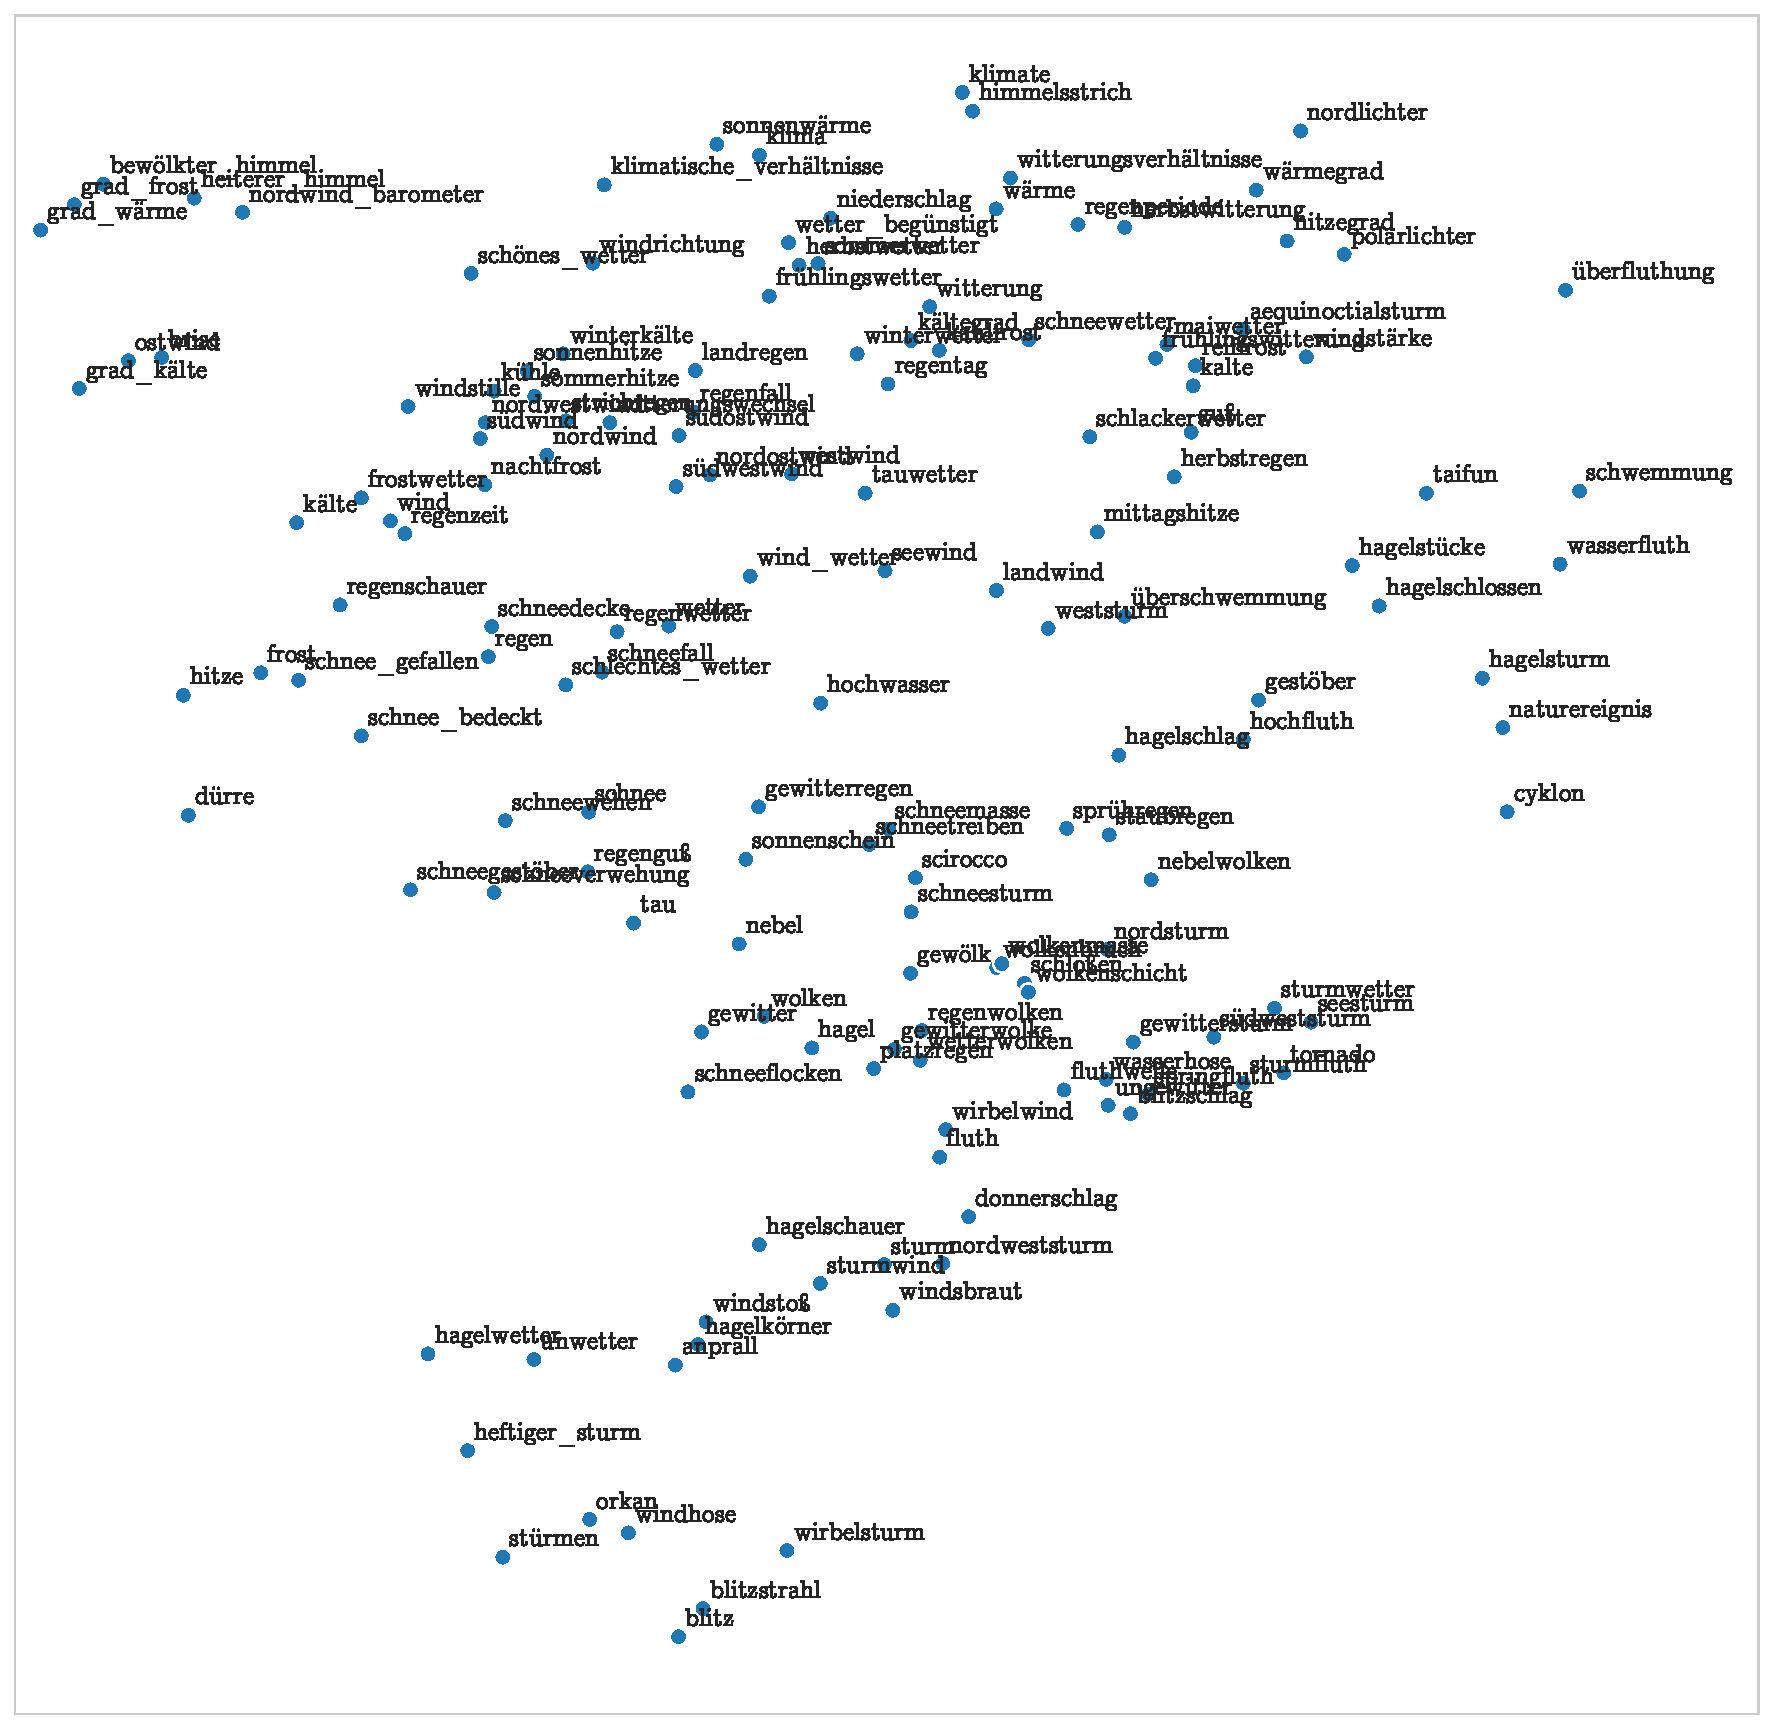
\includegraphics[width=0.9\textwidth]{images/keyword_umap.pdf}
    \caption{Une visualisation spatiale des vecteurs de mots-clés}
    \label{fig:keyword_umap}
\end{figure}

L'on constate que les mots-clés sont regroupés assez intuitivement. Par exemple, la plupart des mots liés à la neige (\textit{schnee}, \textit{schneegestöber}, \textit{schnee\_bedeckt}, \textit{schnee\_gefallen}, etc.) se concentrent autour de la partie gauche du graphique. En haut se trouvent les mots pour le climat et le temps (\textit{klimate}, \textit{klimatische\_verhältnisse}, \textit{witterung}, \textit{frühlignswetter}, etc.). Les concepts liés à la tempête forment un nuage flou autour de la partie inférieure centrale (\textit{wirbelwind}, \textit{nordweststurm}, \textit{tornado}, \textit{sturmwetter}, etc.), pendant que leurs variations plus extrêmes se concentrent en bas du graphique (\textit{heftiger\_sturm}, \textit{orkan}, \textit{wirbelsturm}, \textit{unwetter}). Il existent aussi des conceptes qui se répartissent de manière assez homogène dans le graphique, notamment les mots liés à la pluie et la grêle. Il faut garder à l'esprit que les vecteurs de \textit{doc2vec} ne représentent les relations sémantiques dans aucune façon absolue - au sens strict, la proximité des deux vecteurs dans le graphique est l'expression de la similarité de leurs contextes dans le corpus. L'omniprésence relative de la pluie et la grêle est donc une signe que ces mots apparaissent dans des contextes plus divers. En revanche, les mots dans la partie supérieure gauche (\textit{bewölkter\_himmel}, \textit{grad\_wärme}, \textit{grad\_frost}, \textit{nordwind\_barometer}) sont ceux qui sont très souvent utilisés dans le style répétitif des observations météorologiques.

% embeddings diachroniques ?

En général, l'analyse de la similarité vectorielle ne présente pas des résultats surprenants - les interrelations entre les mots-clés conforment plus ou moins à une compréhension moderne et quotidienne de la terminologie météorologique (à quelques exceptions près, p. ex. le mot mot archaïque pour la tempête, \textit{Windsbraut}. Le vocabulaire créé à l'aide des distances vectorielles et les positionnements des mots dans l'espace vectorielle montrent que les mots liés au climat étaient perçus de façon relativement similaire à celle d'aujourd'hui. 

\clearpage


\subsection{Distribution et tendances des entités \footnote{Les manipulations contenues dans cette section se trouvent dans \texttt{./notebooks/analysis.ipynb}. La classe Python utilisé pour faciliter l'agrégation des données est dans \texttt{./climdist/utils.py}}} \label{entity_distribution}

\begin{wrapfigure}{r}{0.48\textwidth}
  \begin{center}
    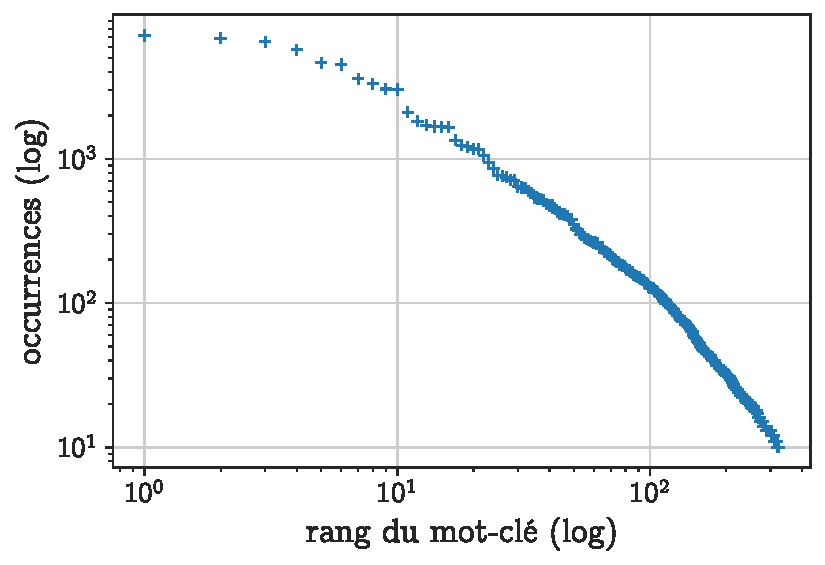
\includegraphics[width=0.48\textwidth]{images/zipf.pdf}
  \end{center}
  \vspace*{-2ex}
  \captionsetup{justification=centering}
  \caption{Nombre des mots-clés par rang sous ses formes originelles}
  \label{fig:zipf}
\end{wrapfigure}

% >>> pretraitement
% Pour les analyses suivantes, seules les entités qui se trouvent dans les articles \og lisibles \fg{} sont prises en compte pour garder une continuité numérique à travers les différentes étapes du travail.

Les 157 mots du vocabulaire ont \textbf{100 938} occurrences au total dans le corpus (ici et ci-après, il s'agit uniquement des formes normalisées), mais leur répartition n'est pas du tout égale. Par exemple, les 6 entités les plus courantes (\textit{Sturm}, \textit{Wind}, \textit{Regen}, \textit{Wetter}, \textit{Witterung}, \textit{Schnee}, \textit{Kälte}) comptent pour 48 714 apparitions, soit presque une moitié de toutes les occurrences. le nombre d'entités ayant plus de 1000 occurrences est 21, tandis que 64 autres entités ont plus de 100 occurrences. En gros, la distribution des entités par rang est celle d'une loi de puissance, où le nombre d'occurrences d'une entité diminue exponentiellement par rapport à son rang de popularité. Une telle répartition, souvent appelée la loi de Zipf, est très courante dans les données de sciences humaines.\footnote{référence M. PETRUSZEWYCZ} La figure \ref{fig:zipf} montre la distribution de fréquences des entités sur une échelle logarithmique - le plus que le courbe se rapproche d'une étroite, le plus la distribution conforme à la loi de Zipf.

Une autre façon de visualiser la distribution, moins théorique mais peut-être plus intuitif, est un nuage de mots (figure \ref{fig:wordcloud}). L'on constate la dominance des mots ayant un rapport au vent (\textit{Wind}, \textit{Sturm}), suivie par trois catégories d'une taille assez égale - les précipitations (\textit{Regen}, \textit{Schnee}), le \og temps \fg{} lui-même (\textit{Wetter}, \textit{Witterung}) et la température (\textit{Kälte}, \textit{Wärme}). A première vue, la distribution conforme alors à une représentation quotidienne du climat et du temps - les mots les plus populaires sont simples et plutôt généraux, comme ceux qui seraient cités par quelqu'un à qui l'on demande à nommer de mots en rapport au temps. Dans le cadre de cette recherche, cette observation banale permet toutefois de constater que le temps ne paraît pas dans la \textit{Rigasche Zeitung} d'une manière catégoriquement différente de notre perception ordinaire, mais aussi, par extension, que la méthode du repérage des entités n'est pas erronée dans ses grandes lignes. %Ce sont alors les détails, les valeurs aberrantes et les changements temporelles auxquelles nous devrons nous concentrer.

\begin{figure}[h]
    \centering
    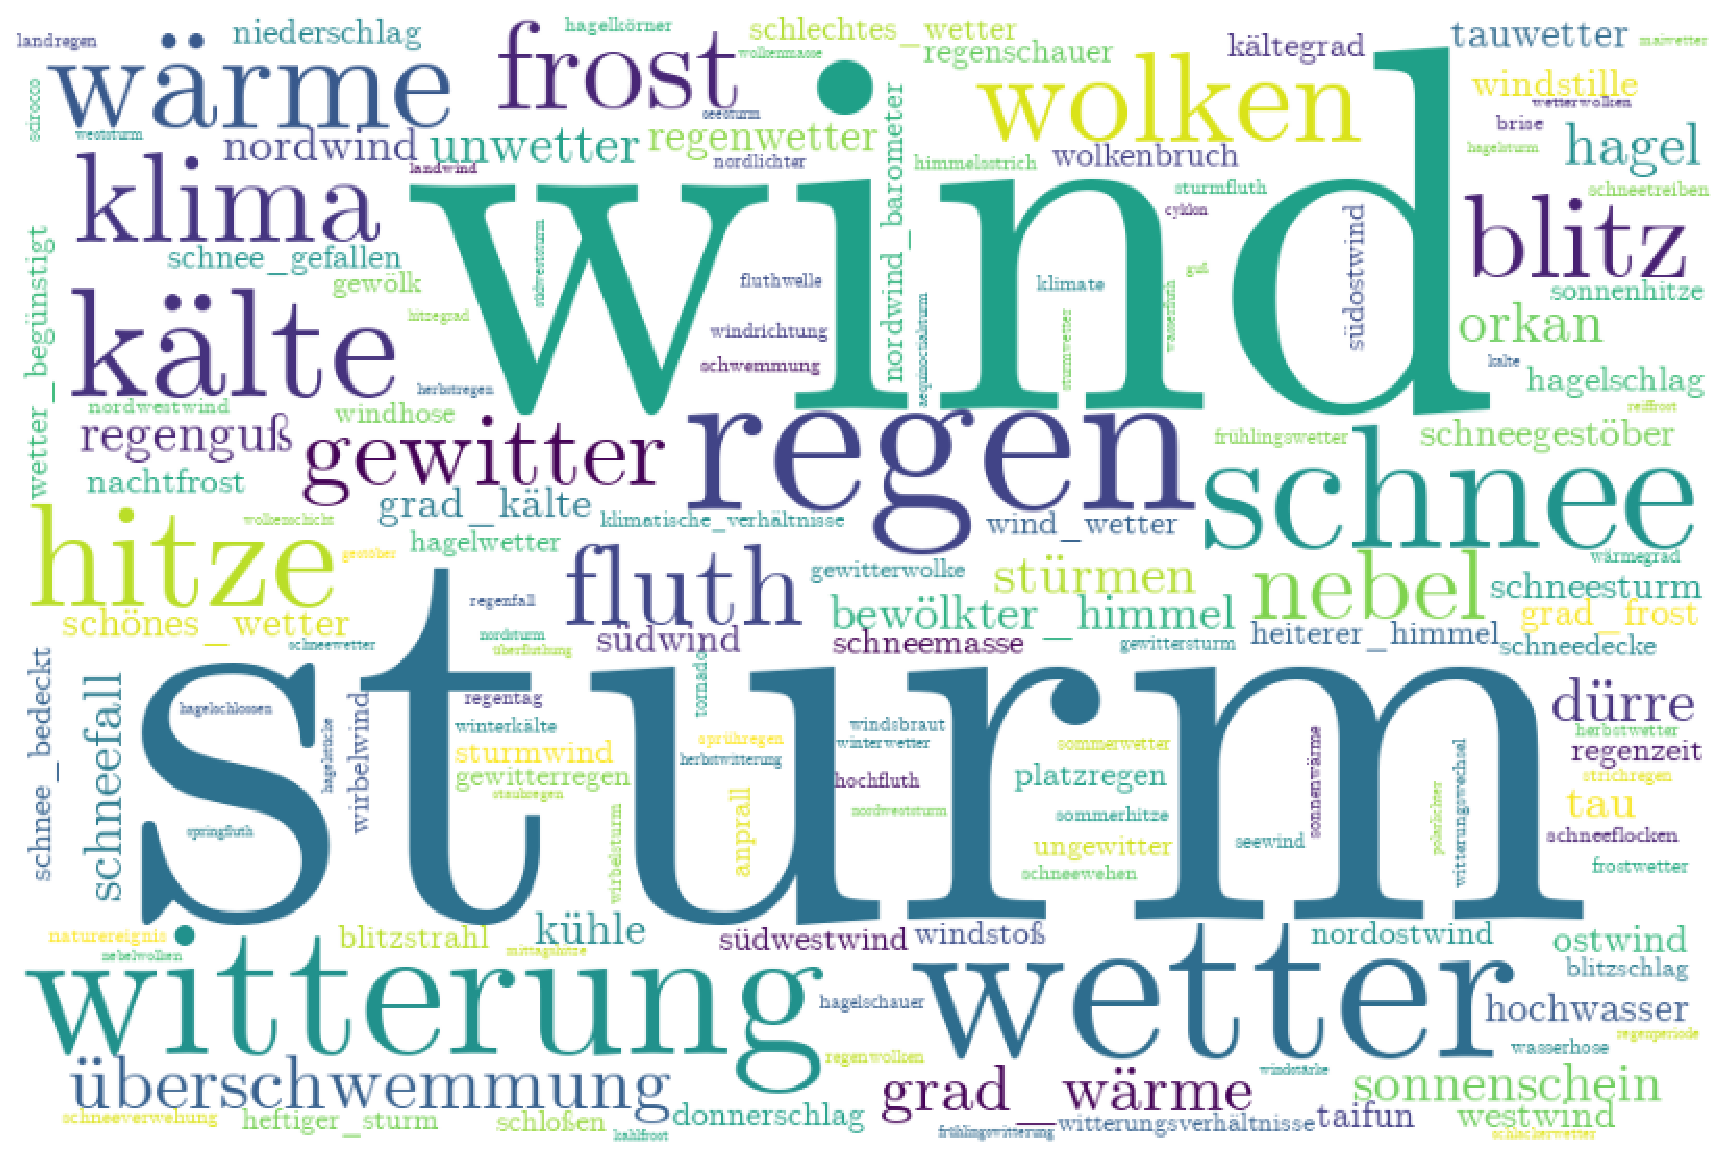
\includegraphics[width=0.9\textwidth]{images/wordcloud_general.pdf}
    \caption{Nuage des mots-clés dans le corpus}
    \label{fig:wordcloud}
\end{figure}

Tout d'abord, l'on peut poser la question \og la fréquence dont l'on parle du climat reste-t-elle stable ? \fg{}. Evidemment, le nombre de mots-clés par an s'augmente au cours du siècle au fur et à mesure que la quantité de l'information devient plus importante (cf. la figure \ref{fig:text_mass}). Pour en tenir compte, le nombre des mots-clés peut être pondéré par la masse totale du texte et présenté sur un graphique. La figure \ref{fig:entities_per_mass} montre la quantité des mots-clés en relation au nombre total de caractères pour chaque année, celui-ci étant une estimation grossière des évolutions de la quantité de l'information. L'on voit que le nombre d'entités en proportion de nombre de la masse textuelle reste relativement stable pendant la période observée. Il existent des pics locaux, plus notamment en 1827, mais en gros, la proportion des entités est toujours dans le même ordre de magnitude. La hausse de l'an 1827 semble être causée par une présence des observations météorologiques dans cette année. Ces observations sont souvent incluses dans d'autres articles à cause d'une erreur (ou un choix) de segmentation et échappent alors au filtre de la qualité d'OCR, car la majeure partie de l'article est toujours lisible. Outre ce biais temporaire, la figure \ref{fig:entities_per_mass} peut être donc interprété comme un indice d'une stabilité relative de la représentation du climat pendant toute la période observée.

\begin{figure}[h]
    \centering
    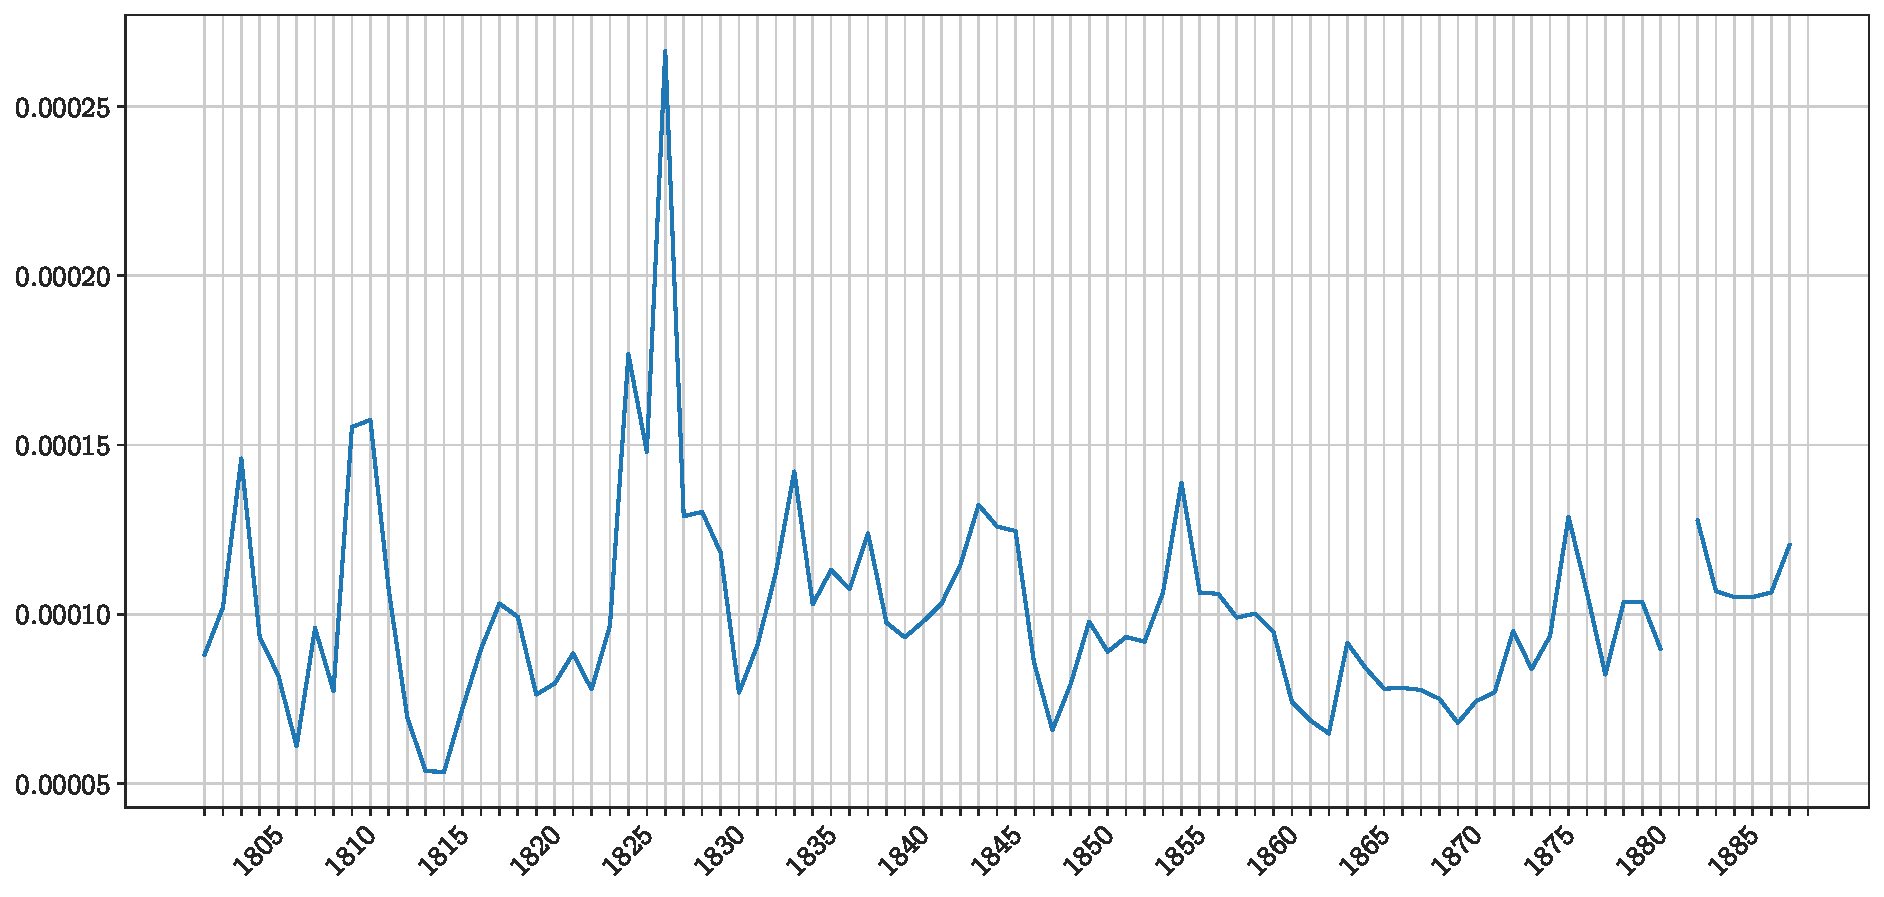
\includegraphics[width=\textwidth]{images/entities_per_mass.pdf}
    \caption{Nombre d'entités par rapport à la masse textuelle en caractères}
    \label{fig:entities_per_mass}
\end{figure}

Il est également possible d'observer la fréquence d'un mot donné et de faire des comparaisons entre différents mots. P. ex., la figure \ref{fig:wetter_witterung_klima} montre la fréquence relative des mots-clés \textit{Klima}, \textit{Wetter}, \textit{Witterung} (climat, le temps, conditions météorologiques) d'une manière relative, i.e. leur proportion de toutes les occurrences d'une année donnée, comme sur les figures \ref{fig:headings_places} et \ref{fig:headings_other}. Là encore, la fréquence d'occurrence semble rester assez stable pour les trois mots et l'on peut en conclure que les catégories terminologiques les plus larges liées au climat one une présence constante dans le journal au cours de la période considérée. Selon les changements locaux les plus importants, l'on remarque le pic du mot \textit{Wetter} dans les années 1860. Un regard plus attentif aux occurrences de \textit{Wetter} dans cette fenêtre temporelle révèle que ils se trouvent en grande majorité (302 fois en 1864-1866) dans les articles intitulés \textit{Börsen- und Handelsnachrichten}, i.e. les actualités boursières et commerciales (cf. le tableau \ref{tab:common_headings} qui relient, entre autres informations, des conditions météorologiques dans d'autres villes. Le début de cette tendance correspond aux développements communicationnels à Riga au début des années 1860 - il est probable que l'arrivée du transport ferroviaire et du télégraphe ont suscité un plus grand intérêt aux conditions météorologiques en temps réel (cf. la setion \ref{sujets_abordes}). Cependant, il ne s'agit pas des observations météorologiques dans le sens \og scientifique \fg{}, mais plutôt des courts remarques: les autres mots-clés ne sont pas mentionnés si souvent que le temps, et une analyse rapide du contexte immédiat du mot en question montre qu'il est le plus souvent décrit avec un seul adjectif, p.ex \textit{schön}, \textit{ruhig}, \textit{trüb} ou \textit{unverändert} (beau, calme, maussade, inchangé).

% ref to the immediate context section?

\begin{figure}[h]
    \centering
    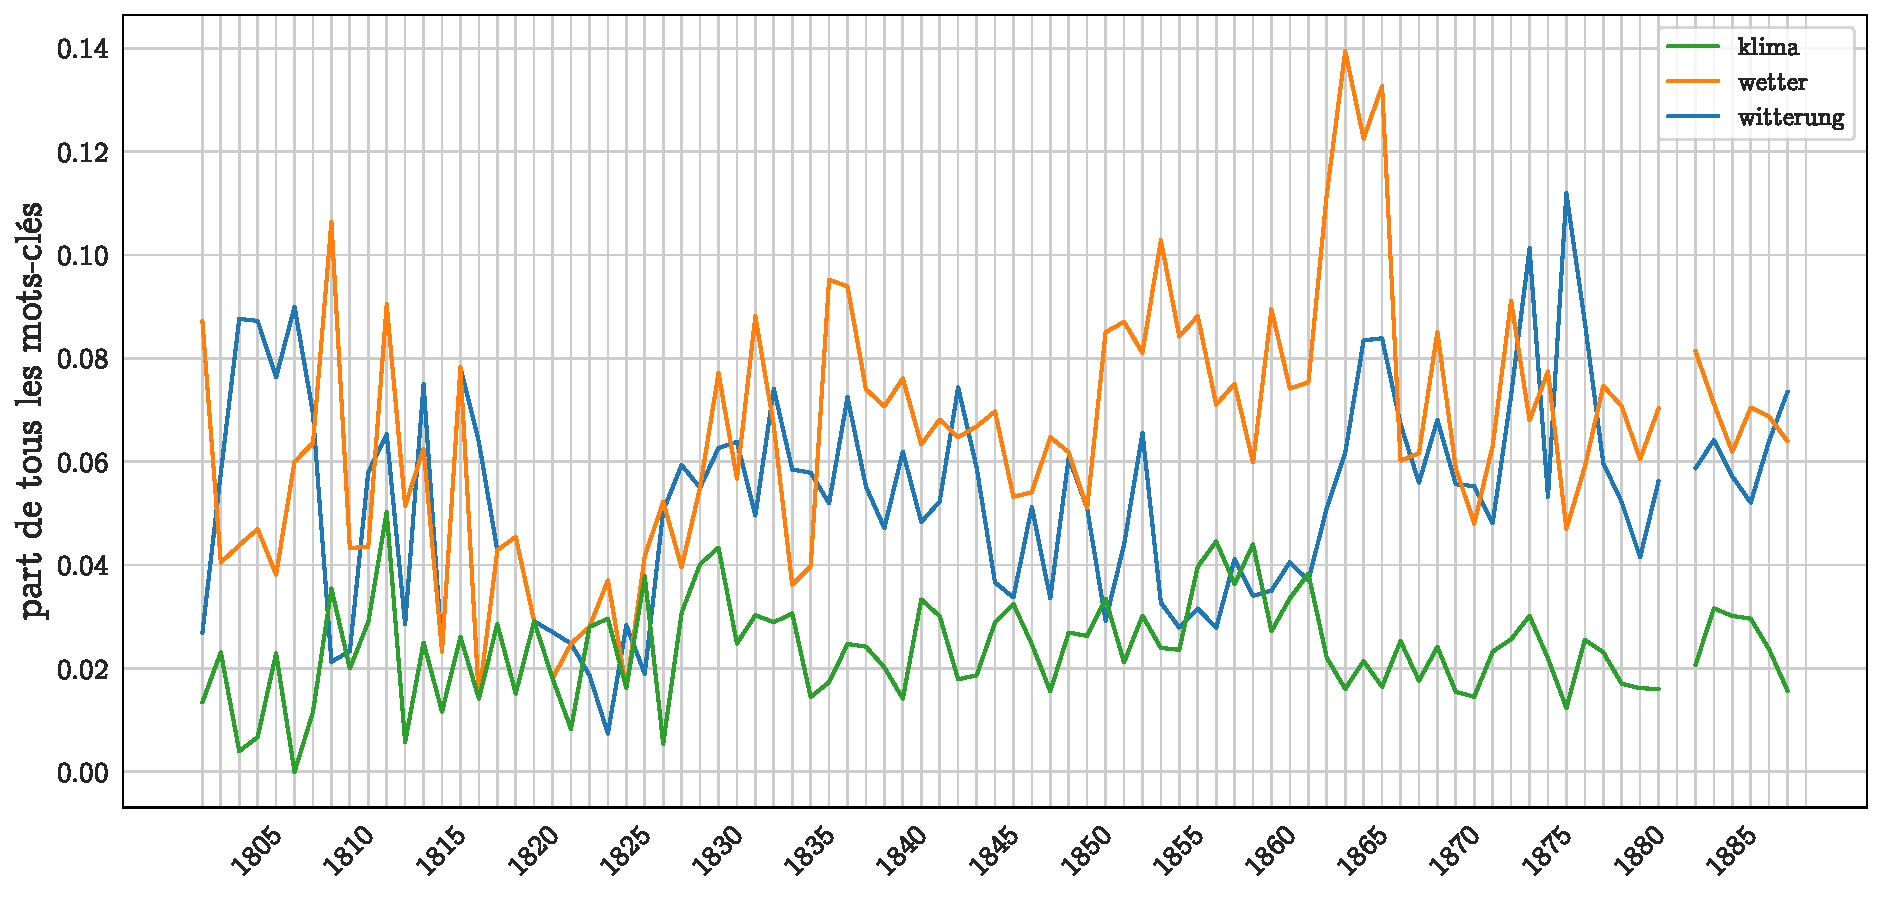
\includegraphics[width=\textwidth]{images/wetter_witterung_klima.pdf}
    \caption{Fréquence relative des mots-clés \textit{climat}, \textit{le temps}, \textit{conditions météorologiques}}
    \label{fig:wetter_witterung_klima}
\end{figure}

Dans le même sens, la distribution des 10 mots-clés les plus populaires est présenté sur la figure \ref{fig:top_keywords10}. En général, l'importance relative de ces mots reste stable pendant la période observée. Le fait que les fluctuations plus importantes se trouvent dans le premier tiers du siècle semble indiquer qu'ils découlent de la faible quantité des données, tandis que la partie du siècle plus riche en données voit une stabilisation de la fréquence de ces mots-clés.

\begin{figure}[h]
    \centering
    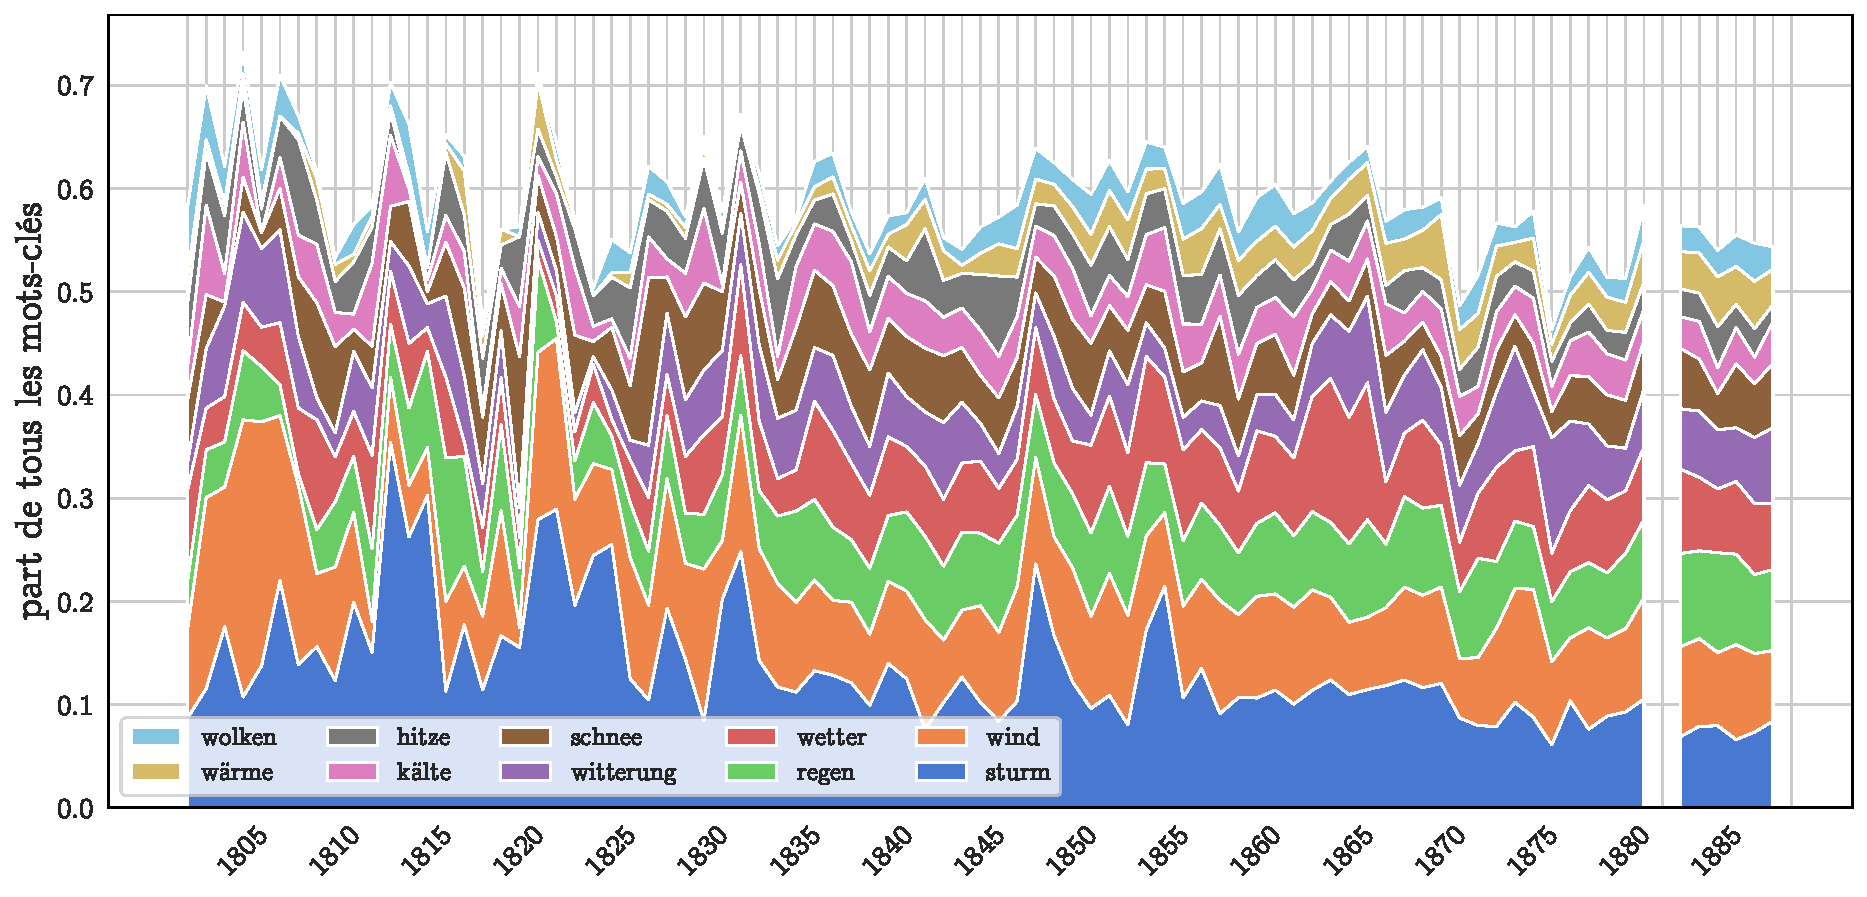
\includegraphics[width=\textwidth]{images/10_most_frequent_ents.pdf}
    \caption{Fréquence relative des 10 mots-clés les plus fréquents}
    \label{fig:top_keywords10}
\end{figure}

Alors que les fréquences des mots-clés les plus fréquents affichent une relative stabilité, les enquêtes sur les mots moins répandus peuvent révéler des poussées temporaires d'intérêt. La figure \ref{fig:orkan_taifun_tornado} démontre les occurrences des mots \textit{Orkan}, \textit{Taifun}, \textit{Tornado} et \textit{Scirocco} sur une échelle absolue. Il se trouve que les occurrences du mot \textit{Orkan} sont reparties de manière assez homogène, mais celles de \textit{Taifun} sont concentrées sur les années 1860 et que \textit{Tornado} ne fait que quelques apparitions, principalement entre 1867 et 1874. En analysant les titres d'articles qui contiennent le mot \textit{Taifun} dans cette fenêtre temporelle, une dominance des actualités de l'Asie est immédiatement perceptible. Il est probable que cette poussée d'intérêt est directement liée aux typhons dévastateurs qui ont ravagé le Japon et la Chine dans les années 1860.\footnote{asian hurricanes references}

Les typhons ne sont pas les seuls phénomènes climatiques tropicales qui trouvent leur chemin vers les lecteurs du \textit{Rigasche Zeitung}. Le Sirocco, un vent saharien qui peut atteindre la vitesse d'un ouragan et parvenir jusqu'au côte nord de la Mediterranée. Les nouvelles sur le Scirocco viennent donc principalement de l'Italie et ses villes. A trois occasions, un article entier est consacré au Scirocco.\footnote{RZ 128124, 1855-10-19; 128224, 1855-10-27; 190735, 1869-04-08}

\begin{figure}[h]
    \centering
    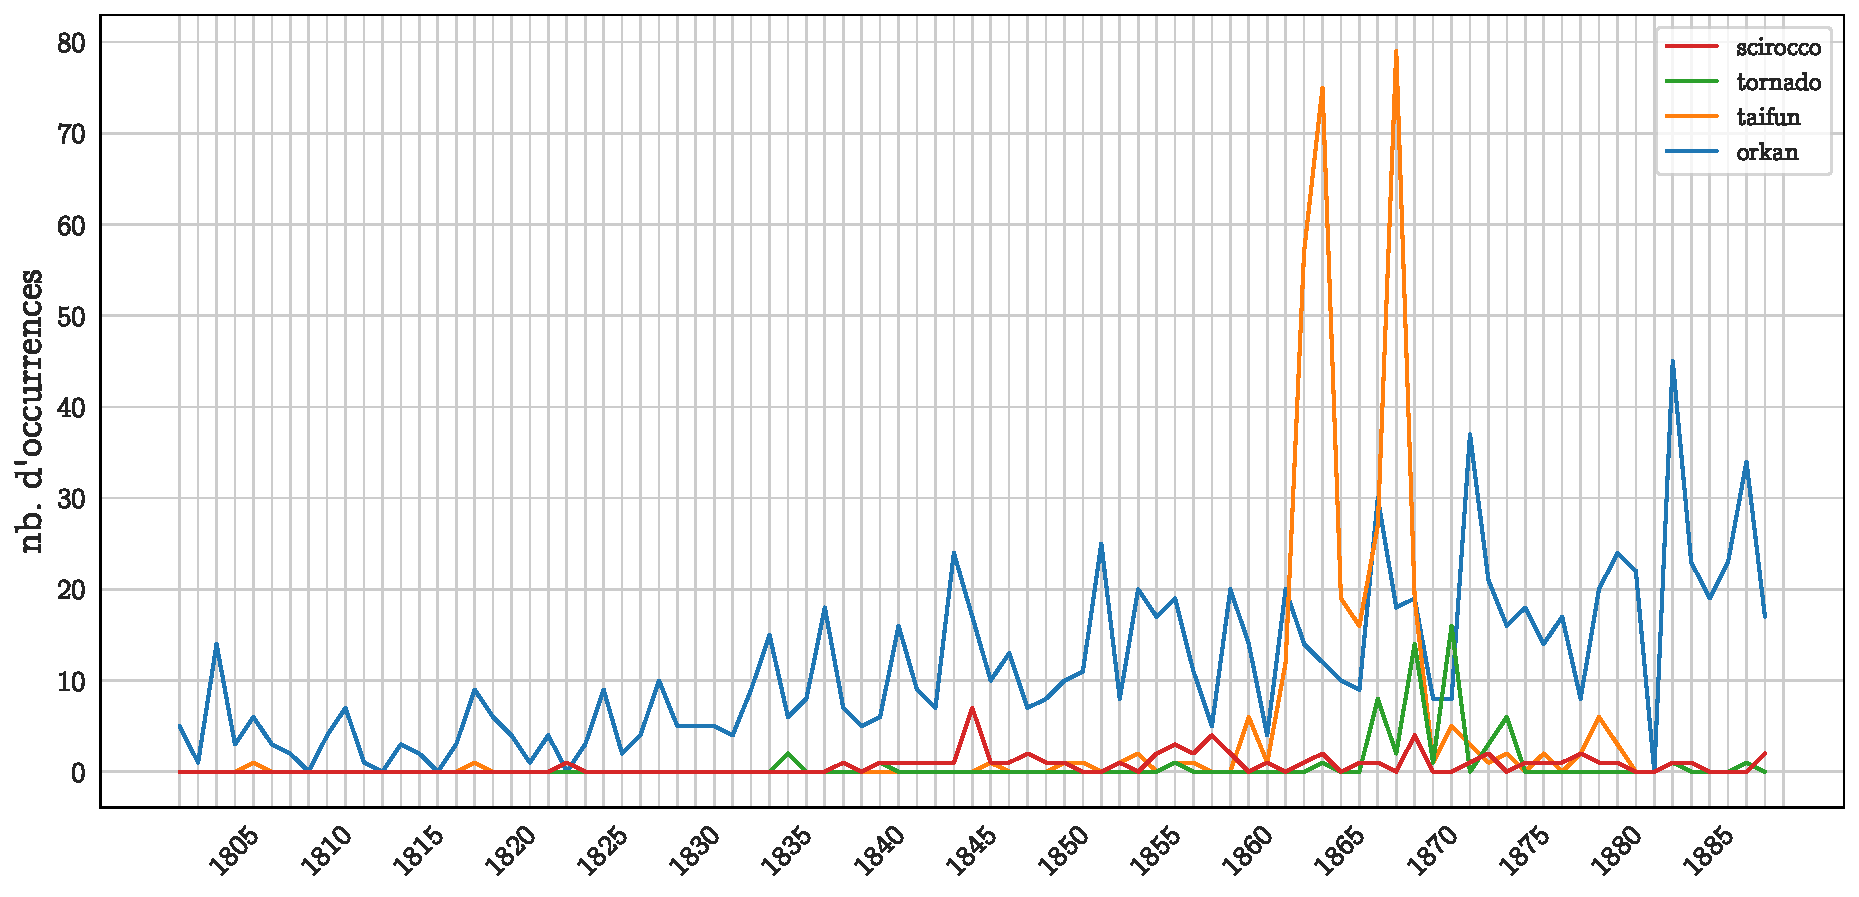
\includegraphics[width=\textwidth]{images/orkan_taifun_tornado.pdf}
    \caption{Fréquence absolue des mots \textit{ouragan}, \textit{typhon}, \textit{tornade}}
    \label{fig:orkan_taifun_tornado}
\end{figure}

D'autres phénomènes présentent encore un image différent. Par exemple, la grêle est le plus souvent mentionnée dans un contexte de l'empire Russe ou de la région Baltique. Un tiers de tous les articles qui contiennent la grêle ou l'un de ses synonymes, sont intitulés \textit{Inland}. Il parait que pendant certaines périodes, des nouvelles des grêles dévastatrices ont circulé dans la presse - p. ex. la figure \ref{fig:hagelschlag} montre que dans le contexte immédiat du mot-clé \textit{Hagelschlag} (coup de grêle), se trouvent les mots \textit{Gouvernement} et \textit{Kreise} (des divisions administratives), ainsi que \textit{shaden}, \textit{schaden\_angerichtet}, \textit{vernichtet}, \textit{Fenstercheiben} et \textit{Getreide} (dommages, dommages causés, détruit, vitres, céréales). \label{about:hagel}

\begin{figure}[h]
    \centering
    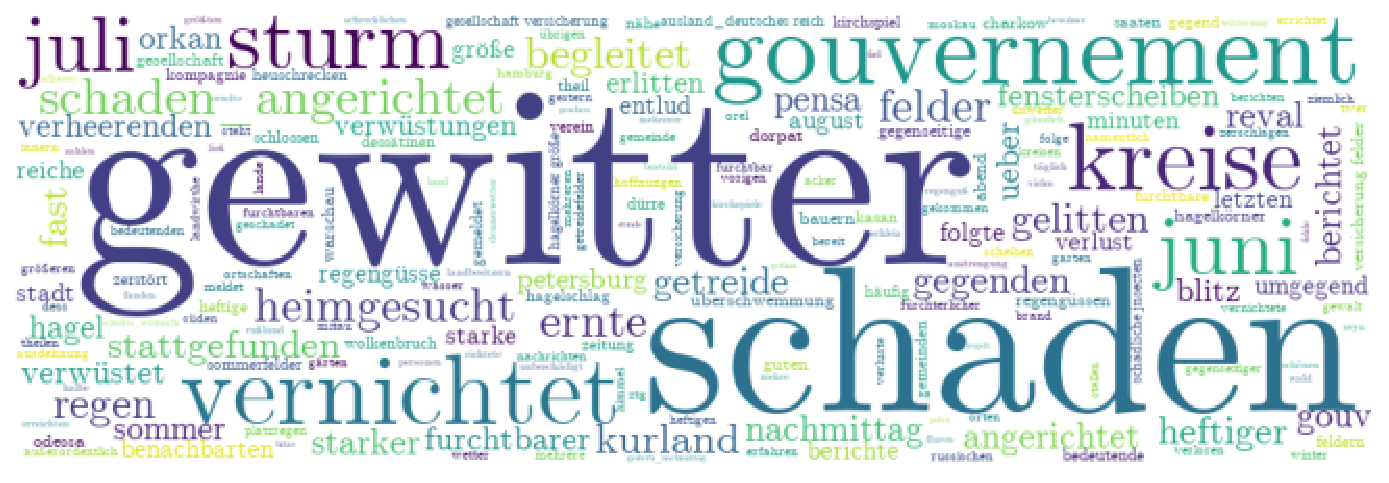
\includegraphics[width=0.9\textwidth]{images/wordcloud_hagelschlag.pdf}
    \caption{Contexte immédiat du mot-clé \textit{Hagelschlag} (coup de grêle)}
    \label{fig:hagelschlag}
\end{figure}

En regardant la fréquence absolue de la grêle et ses synonymes (figure \ref{fig:hagel}), l'on remarque immédiatement un pic soudain dans l'année 1872. Il s'avère que la poussée est causée en grande partie due à deux articles qui contiennent au total 20 mentions de grêle, ainsi qu'un grand nombre d'autres mots-clés. Ces articles, à une semaine d'intervalle, racontent dans le détail une tempête de grêle qui a ravagé Riga et ses alentours le 10 mai 1872. Le deuxième article semble en fait être un supplément du journal, entièrement consacré à ces événements. La grêle fût accompagné par un tourbillon de poussière et infligea des dommages considérables.\footnote{\og Un événement naturel si rare a frappé une partie de notre province, notamment notre ville et ses environs, et a laissé des traces de destruction si cruelles qu'il semble justifié de mettre par écrit les impressions encore vives et de laisser une image de ses conséquences, même pour les temps ultérieurs, \fg{} rapporte le correspondant du \textit{Rigasche Zeitung} émotionnellement. RZ 19/03/1872 (\texttt{id: 208050})} Parmi les dommages constatés, arbres déracinés, fenêtres cassées, jardins en ruine ont été signalés, ainsi que la mort de plusieurs personnes.\footnote{\og Je viens d'apprendre avec certitude que quatre domestiques du château de Wenden ont été entièrement détruits, et qu'il ne reste pas une poutre sur l'autre. Une femme a été tuée et on n'a retrouvé jusqu'à présent qu'un bras ou une jambe d'une gardienne, dont on cherche le corps. On dit aussi que les domestiques de Freydenhof et de Lindenhof ont été détruits et qu'un petit bois de bouleaux a été totalement déraciné et bouleversé. \fg{} RZ 13/03/1872 (\texttt{id: 207965})} Les deux articles sont un curieux mélange des narrations émotionnelles probablement un peu exagérées et des descriptions minutieuses de la nature du phénomène, communicant au lecteur les changements de la température et de la pression atmosphérique et décrivant la taille précise des plus gros grêlons trouvés.

\begin{figure}[h]
    \centering
    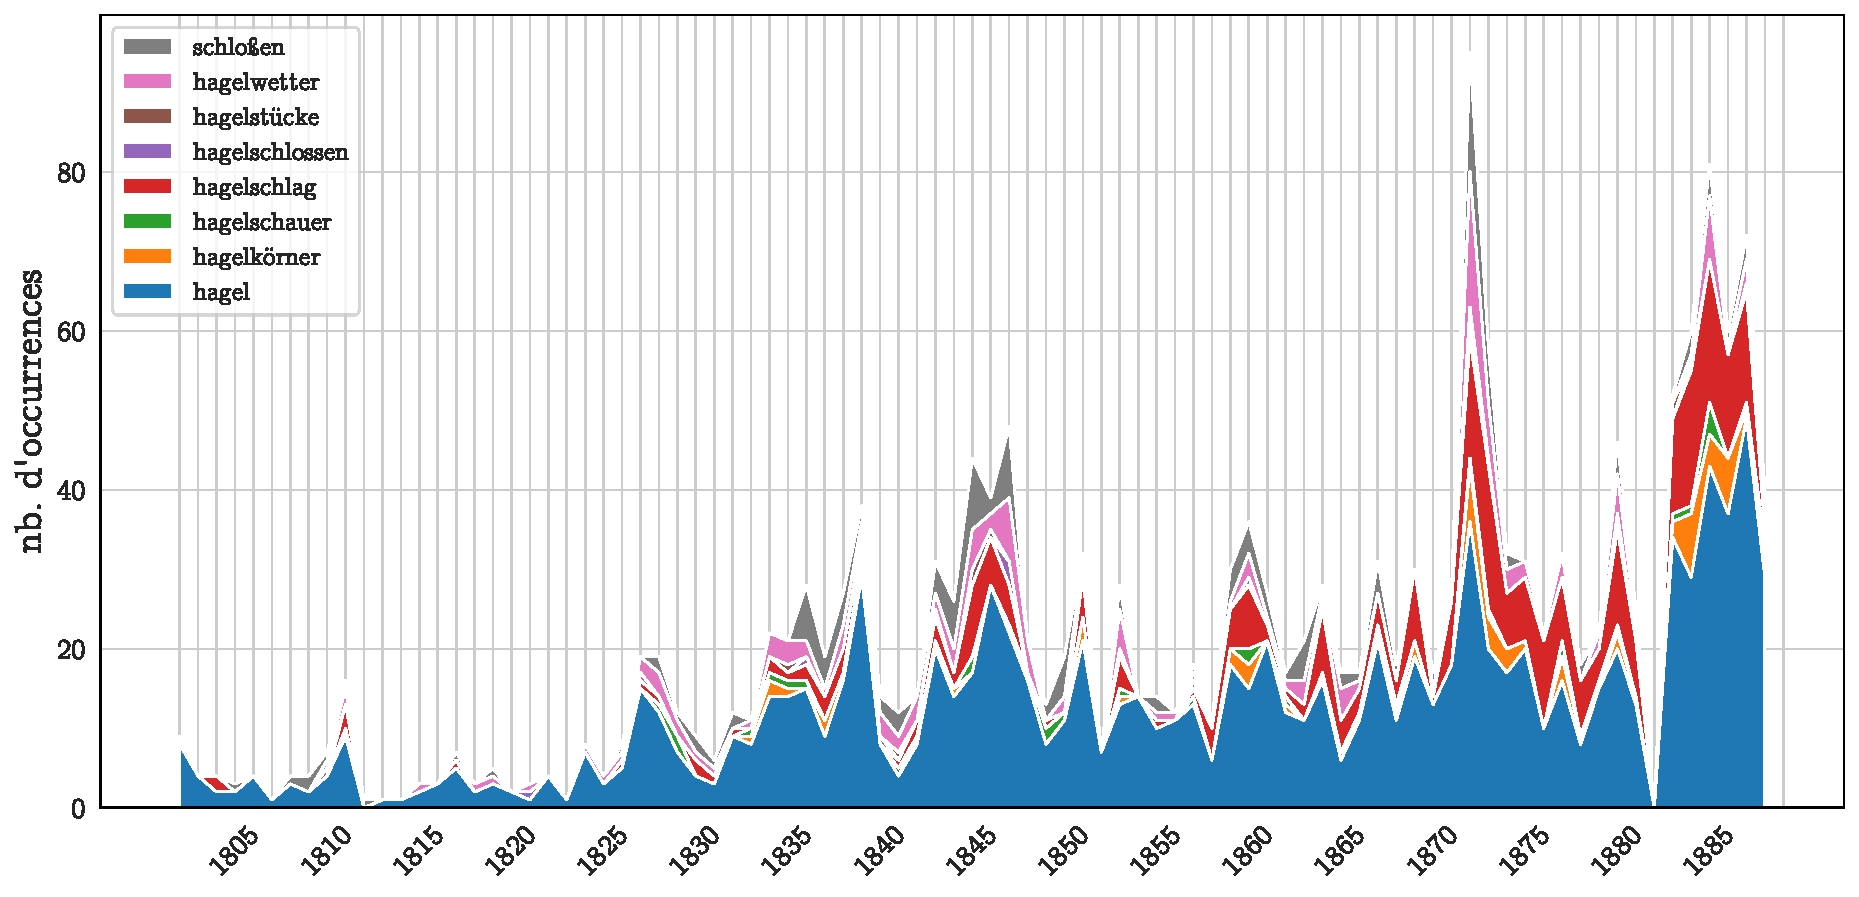
\includegraphics[width=\textwidth]{images/hagel.pdf}
    \caption{Fréquence absolue de \textit{grêle} et ses synonymes}
    \label{fig:hagel}
\end{figure}

Comme le montre cet exemple, les tendances temporelles des mots clés peuvent également servir à la détection des événements uniques qui peuvent ensuite être analysés à l'aide des métadonnées. Toutefois, il faut prêter attention aux réserves que peut susciter un petit nombre de textes contenant un nombre élevé de mots-clés. En regardant la figure \ref{fig:hagel}, l'on pourrait d'abord avoir l'idée que l'année 1872 a connu d'abondantes tempêtes de grêle, mais en réalité, cette dynamique est surtout due à une forte surreprésentation du phénomène dans deux articles.

Le dernier exemple de ce chapitre démontre les pièges qui peuvent surgir si l'analyse quantitative est trop superficielle. La fréquence du mot \textit{Sturm} (tempête) et ses synonymes est la plus élevée en 1855 avec 457 occurrences, tandis que la fréquence moyenne en 1802-1888 est de 161 par an. Une simple analyse montre tout de suite la raison de ce pic. En comparant les mots voisins du phénomène, on voit les différences entre le nuage de mots calculé sur toute la période et le nuage de mots basé uniquement sur les données de 1855. Les mots les plus présents dans le nuage général semblent indiquer que de l'information sur les tempêtes a été souvent communiquée juste après un événement important dans une autre ville (\textit{Stadt}, \textit{letzten}, \textit{Nacht} - ville, dernière, nuit). Des autres mots marquent des liaisons à la navigation (\textit{Schiff}, \textit{Küste}, \textit{Hafen}, \textit{Wasser} - navire, côte, port, eau) et les caractéristiques des tempêtes fortes (\textit{heftigen}, \textit{wüthete}, \textit{furchtbarer} - violent, faire rage, terrible). Entre 1802 et 1888, les mots de contexte donnent une image assez cohérente de la représentation des tempêtes en tant qu'événements météorologiques dans le corpus.

\begin{figure}[h!]
\centering
\begin{subfigure}
    \centering
    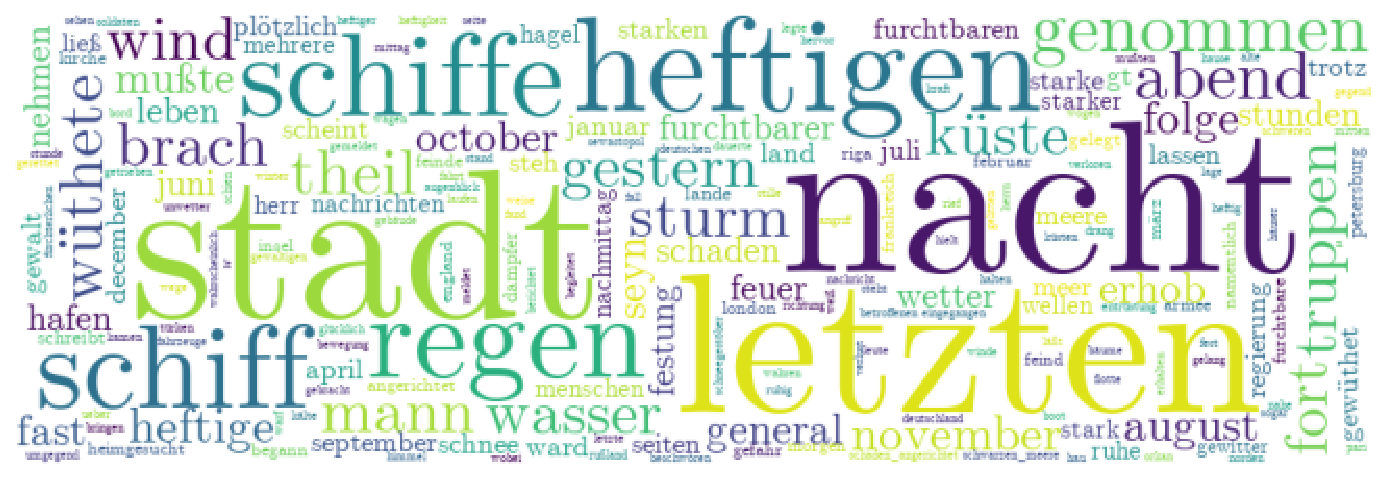
\includegraphics[width=0.9\textwidth]{images/wordcloud_sturm.pdf}
\end{subfigure}
\begin{subfigure}
    \centering
    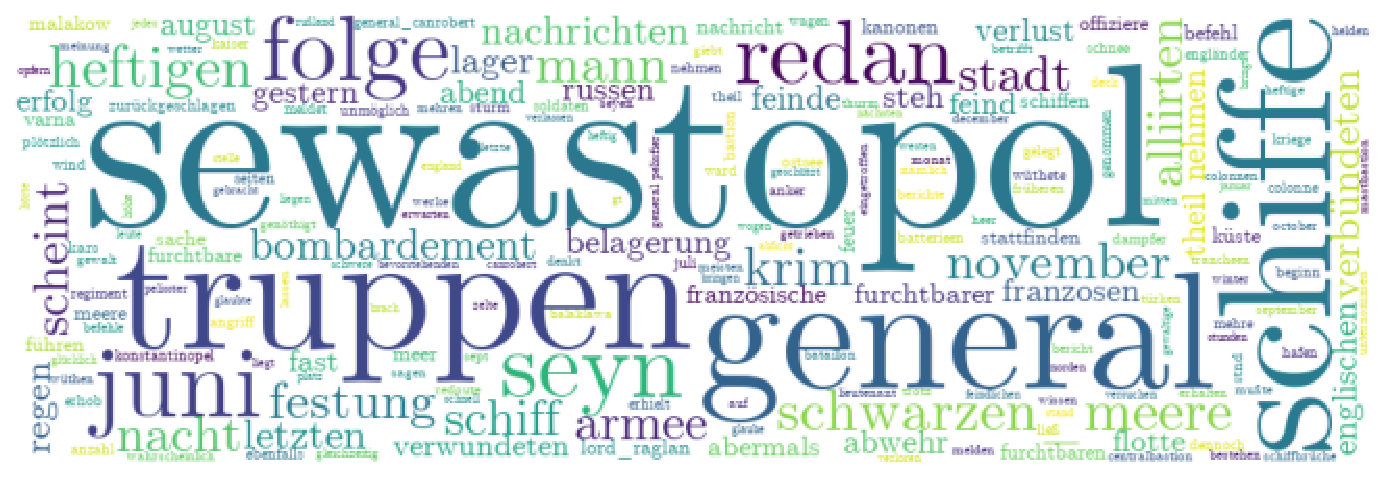
\includegraphics[width=0.9\textwidth]{images/wordcloud_sturm_1855.pdf}
\end{subfigure}
\caption{Le contexte immédiat de \textit{tempête} pour toute la période et en 1855}
\label{fig:sturm_wordclouds}
\end{figure}

Par contre, le second nuage trahit d'emblée en quoi il serait faux de considérer le pic de 1855 comme un indice de tempêtes violentes ou plus fréquentes. Les mots \textit{Sewastopol} \textit{Truppen}, \textit{General}, \textit{Bombardement}, \textit{Belagerung}, \textit{Krim}, \textit{Franzosen} etc. font clairement apparaître qu'il s'agit du sens militaire du mot \textit{Sturm}, dont la fréquence a été augmentée par la guerre de Crimée.

La notion du contexte est donc très importante pour la lecture distante du climat et sera traitée dans la partie suivante. En parallèle, le chapitre actuel démontre les diverses possibilités d'analyse quantitative au niveau des mots-clés. Les distributions temporelles des mots-clés révèlent de l'information sur la quantité et la nature de la représentation des événements climatiques. Dans certains cas, il est possible de identifier des événements uniques qui permet d'accéder à une analyse qualitative des sources.

\clearpage


\section{Sujets du climat} \label{topic_modeling}

Comme démontré dans le chapitre précédent, la nature des textes qui contiennent des mots-clés pertinents peut varier considérablement, un certain nombre d'eux n'ayant même aucun rapport avec le climat. Etant donné que les descriptions du temps et le climat sont évidemment très différentes, le but de ce chapitre est de modéliser les catégories principales des textes contenant des mots-clés \og climatiques \fg{}.

La modélisation de sujets est un ensemble de techniques qui permettent détecter automatiquement les \og sujets \fg{} qui apparaissent dans une collection de documents. Il s'agit des méthodes non-supervisées, ce qui veut dire qu'ils fonctionnent sans données étiquetées. Plus notamment, il n'est pas nécessaire de prédéterminer les types de texte que l'on s'attend à trouver - les sujets sont modelés selon la distribution des mots dans les textes. Ainsi, une co-occurrence répétitive d'un nombre de mots a la chance d'être définie comme un sujet. Les noms des sujets trouvés par l'algorithme dépendent ainsi de l'interprétation humaine. Leur caractère non-supervisée est donc l'avantage principal des techniques de modélisation de sujets, parce qu'ils permettent d'explorer la nature des textes sans connaissance préalable sur leur contenu. Pour un grand corpus, des attentes erronées concernant les thèmes évoquées pourrait même gravement fausser les résultats.

Il existe plusieurs méthodes de modélisation des sujets, qui se distinguent les unes des autres principalement par la nécessité de disposer d'un nombre prédéterminé de sujets. Après quelques expériences, notamment une approche LDA\footnote{LDA ref} qui a échoué, j'ai découvert que les meilleurs résultats sont obtenus par une méthode relativement nouvelle appelée \textit{top2vec}. \textit{Top2vec} est basé sur \textit{word2vec} qui a été utilisé dans le chapitre précédent pour vectoriser les mots du corpus. Tout d'abord, \textit{top2vec} calcule des embeddings supplémentaires pour les documents - ceux-ci sont basés sur les valeurs des embeddings de mots dans le document. Les vecteurs hyperdimensionnels de documents obtenus sont ensuite projetés dans un espace bidimensionnel avec l'algorithme UMAP (de la même manière que pour la figure \ref{fig:keyword_umap}). Enfin, les vecteurs bidimensionnels obtenus sont regroupés par HDBSCAN, un algorithme de regroupement (\textit{clustering}) qui trouve les zones où les vecteurs sont le plus densément regroupés.\footnote{HDBSCAN ref} Cela repose sur l'hypothèse que les documents ayant des vecteurs similaires (c'est-à-dire proches les uns des autres dans l'espace) sont similaires dans leur contenu sémantique. Chaque regroupement trouvé par HDBSCAN est donc considéré comme un \og sujet \fg{}. Les documents ne doivent pas nécessairement appartenir à un seul sujet. Par exemple, les vecteurs qui se trouvent entre deux zones denses sur la projection UMAP sont considérés comme appartenant partiellement aux deux \textit{clusters}, celui dont il est le plus proche étant le sujet principal. Les sujets résultants sont définis par les mots qui leur sont les plus caractéristiques.\footnote{top2vec ref}

Afin d'utiliser \textit{top2vec} sur des descriptions climatiques et météorologiques, il est d'abord nécessaire d'extraire les parties des articles qui contiennent les mots-clés pertinents. Ces parties de texte deviennent alors l'entrée de l'algorithme de modélisation des sujets. Les segments ont été créés en tenant compte de certains paramètres : dans les textes tokenisés, les 20 mots qui précèdent et suivent un mot-clé ont été inclus dans l'intervalle. En outre, si la distance entre deux mots-clés était égale ou inférieure à 100 \textit{tokens}, tous ces \textit{tokens} étaient inclus dans l'intervalle. Cela devrait permettre de créer des segments plus cohérents et plus longs dans les cas où les mots-clés mentionnés ne sont pas étroitement groupés. Enfin, seuls les espaces qui incluent trois mots-clés ou plus sont utilisés pour la modélisation du sujet. Cela réduit la variance textuelle en omettant les mots-clés isolés - plusieurs mots-clés apparaissant ensemble augmentent considérablement la probabilité que le mot-clé ne soit pas utilisé dans un sens métaphorique, par exemple.\footnote{\texttt{./climdist/train\_top2vec.py}, fonction \texttt{build\_spans}, paramètres \texttt{window}, \texttt{stretch}, \texttt{min\_len}}

Les paramètres décrits ont un effet important sur l'éventuelle modélisation du sujet car ils tentent d'isoler efficacement les descriptions climatiques et météorologiques du texte environnant. Cela n'est malheureusement pas toujours possible avec un ensemble de règles fixes, car les descriptions réelles dans le corpus varient considérablement en longueur et sont souvent entourées de toutes sortes de textes différents. Comme décrit dans le chapitre 1, la séparation des articles est très dépendante des décisions humaines et de nombreux articles contiennent une variété de nouvelles et de messages. Ainsi, il est inévitable que certaines des travées résultantes comprennent des parties non pertinentes de l'article et que certaines descriptions pertinentes plus longues soient divisées en plusieurs segments. Des expérimentations supplémentaires avec ces valeurs pourraient donc potentiellement aider à améliorer les résultats à l'avenir.

Les segments sont utilisés pour entraîner le modèle \textit{top2vec}. Celui-ci attribue un vecteur de document à 300 dimensions à chaque segment et ne prend en compte que les mots qui apparaissent au moins 20 fois. Le nombre original de sujets détectés par l'algorithme est de 46 \label{46_topics}, mais \textit{top2vec} permet de réduire ce nombre pour obtenir une vue plus générale. Cela se fait en fusionnant les \textit{clusters} les plus similaires jusqu'à ce que le nombre de sujets souhaité soit atteint. Après avoir expérimenté avec différents nombres, j'ai trouvé que le nombre optimal de sujets qui est facilement interprétable tout en gardant un niveau de détail suffisant, est de 16. Après un examen des mots les plus caractéristiques de chaque sujet, sa distribution temporelle, ses mots-clés les plus répandus et les titres des articles dans lesquels les segments sont contenus, ainsi que plusieurs exemples de textes, j'ai attribué un nom à chacun d'entre eux.

Sur les 16 sujets, quatre peuvent être considérés comme des faux-positifs. Cela signifie qu'ils contiennent les mots-clés pertinents mais que le sujet en général indique qu'ils sont utilisés soit dans un sens métaphorique, soit qu'ils résultent de segments \og bruyants \fg{}. Par exemple, deux sujets contiennent principalement des textes de nature littéraire et souvent inclus dans des romans qui étaient parfois publiés en partie dans le \textit{Rigasche Zeitung}. Deux autres sujets sont de nature politique, souvent inclus en raison du sens métaphorique du mot \textit{Sturm} - plus particulièrement dans son sens militaire (voir page \pageref{fig:sturm_wordclouds}). Il en reste donc 12 sujets différents auxquels j'ai donné les étiquettes suivantes (présentés par ordre de taille) :

\vspace{1ex}
\begin{enumerate}
    \item chimie-végétation
    \item récolte
    \item féstivités
    \item commerce
    \item navigation
    \item hiver-ferroviaire
    \item inondation
    \item télégrammes
    \item tempête-grêle
    \item science
    \item düna
    \item foudre-incendie
\end{enumerate}
\vspace{2ex}

La section suivante du travail détaille les 12 sujets un par un, en présentant leurs mots les plus caractéristiques, les mots-clés climatiques qui y apparaissent le plus souvent et leur répartition temporaire. En outre, l'un des textes les plus exemplaires pour chaque sujet est présenté - il est choisi parmi les 1-5 segments dont les vecteurs sont les plus centrales dans le groupe (sujet) auquel ils appartiennent. Le chapitre se termine par une analyse comparative des résultats concernant chaque sujet.

\clearpage


\subsection{Chimie-végétation} \label{topic1_chimie-vegetation}

\begin{figure}[H]
\centering
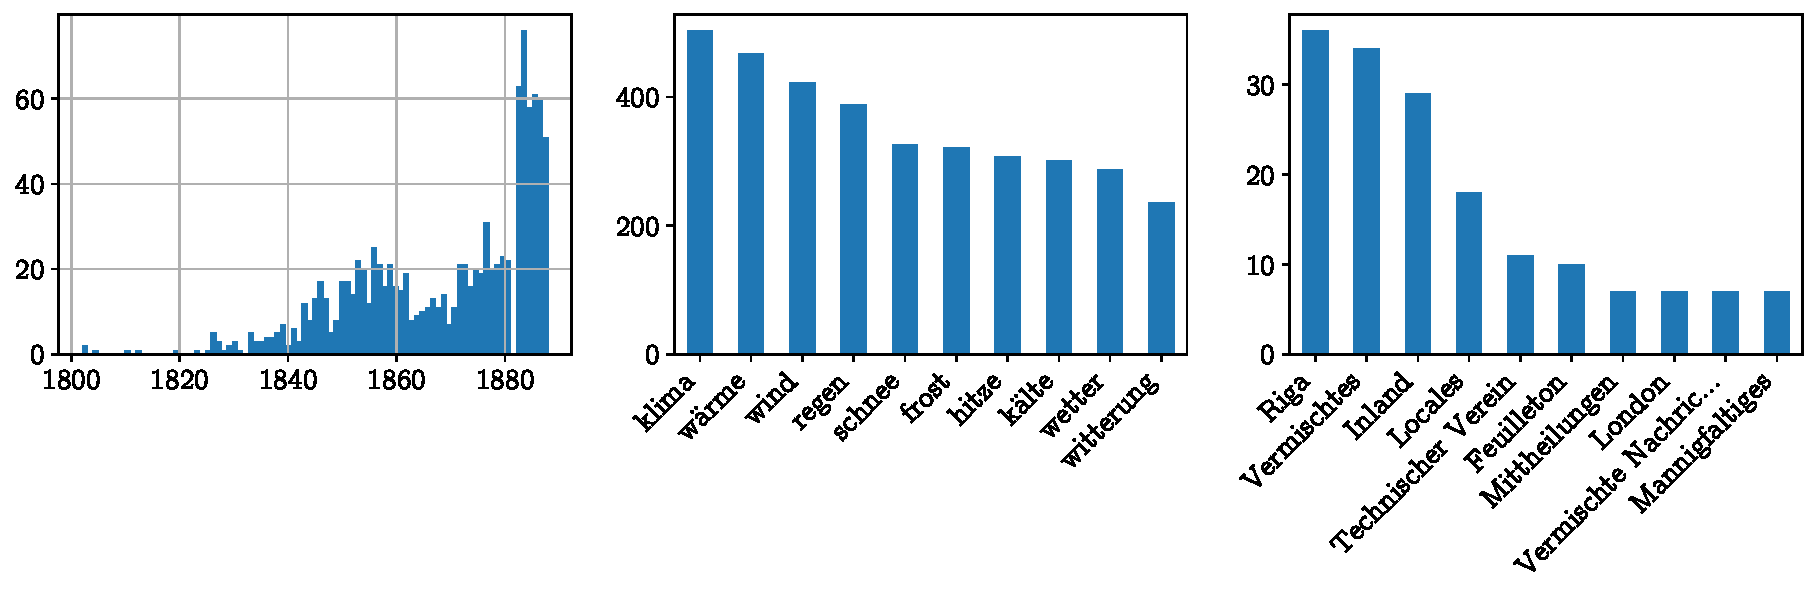
\includegraphics[width=\textwidth]{images/topic_charts_1.pdf}
\end{figure}

\begin{flushleft}
\textbf{Taille :} 1053 segments

\textbf{Mots caractéristiques :} \texttt{pflanzen}, \texttt{klima}, \texttt{pflanze}, \texttt{bodens}, \texttt{boden}, \texttt{moglichst}, \texttt{warme}, \texttt{anwendung}, \texttt{dunger}, \texttt{feuchtigkeit}, \texttt{oberflache}, \texttt{beziehung}, \texttt{winter}, \texttt{weise}, \texttt{giebt}, \texttt{besteht}, \texttt{gewohnlich}, \texttt{entwickelung}, \texttt{bildet}, \texttt{liefert}, \texttt{anlage}, \texttt{stoffe}, \texttt{ausgesetzt}, \texttt{erwarmung}, \texttt{regel}, \texttt{saat}, \texttt{erforderlich}, \texttt{verdunstung}, \texttt{falle}, \texttt{wurzeln}.
\end{flushleft}

\noindent Ce thème, qui est aussi le plus nombreux, est moins cohérent que les suivants et il contient en fait plusieurs types de textes. Il y a des descriptions chimiques qui sont incluses en raison de la nature générale de mots comme \textit{nature} et \textit{chaleur}, et qui pourraient donc être considérées comme des faux positifs. Un autre type de segments traite de l'agriculture de manière technico-scientifique. Enfin, les textes sur la récolte sont aussi parfois classés comme appartenant à ce thème, alors qu'ils pourraient en fait appartenir au sujet suivant.

\medskip

\noindent \textbf{Exemple 1 :} \textit{Il faut compter environ trois à quatre semaines, selon la variété de pomme de terre et les conditions météorologiques, avant que les plantes ne sortent de terre. Pendant ce temps, les conditions météorologiques, les mauvaises herbes, etc. peuvent déjà endommager les plantes ou du moins influencer leur croissance.}\footnote{RZ 11/06/1887 (\texttt{id: 282166})}

\noindent \textbf{Exemple 2 :} \textit{Seule la pratique et les différentes conditions locales peuvent déterminer s'il est indiqué, en toutes circonstances, de faire précéder la carbonisation de la sole sèche à l'air. La quantité importante d'eau hygroscopique contenue dans une telle tourbe (au moins 20\%) nécessite une dépense de combustible correspondante pour son évaporation lors de la carbonisation. Lorsque la chaleur nécessaire à la carbonisation est produite par la combustion d'une partie du matériau de carbonisation} [...].\footnote{RZ 28/07/1877 (\texttt{id: 235631})}

\clearpage



\subsection{Récolte} \label{topic2_recolte}

\begin{figure}[H]
\centering
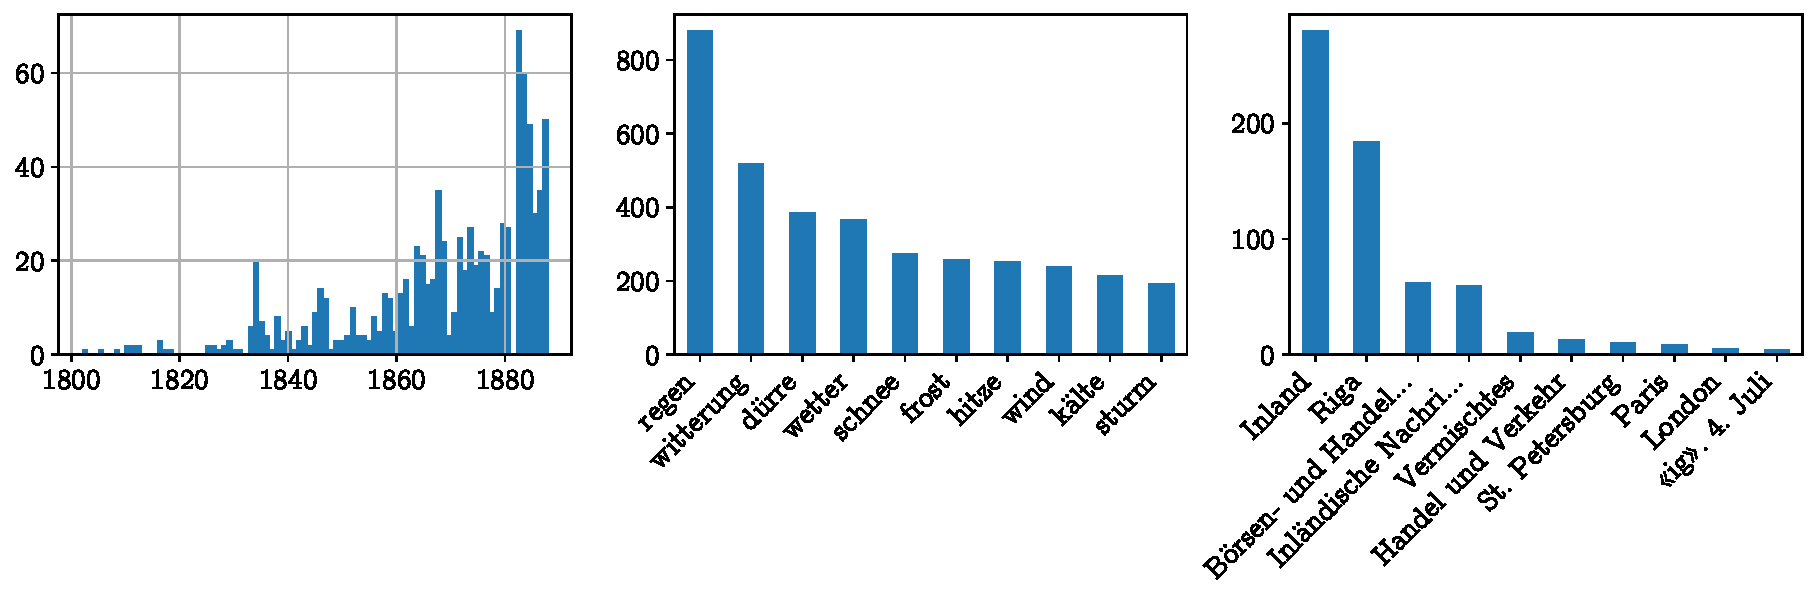
\includegraphics[width=\textwidth]{images/topic_charts_2.pdf}
\end{figure}

\begin{flushleft}
\textbf{Taille :} 887 segments

\textbf{Mots caractéristiques :} \texttt{ernte}, \texttt{durre}, \texttt{heuernte}, \texttt{ertrag}, \texttt{sommergetreide}, \texttt{mittelmaßige}, \texttt{sommerkorn}, \texttt{felder}, \texttt{wintergetreide}, \texttt{mittelmaßig}, \texttt{sommersaaten}, \texttt{korn}, \texttt{graswuchs}, \texttt{kreise}, \texttt{verspricht}, \texttt{saat}, \texttt{gelitten}, \texttt{wintersaaten}, \texttt{befriedigend}, \texttt{klee}, \texttt{wachsthum}, \texttt{aussaat}, \texttt{wintersaat}, \texttt{roggen}, \texttt{roggenernte}, \texttt{geschadet}, \texttt{saaten}, \texttt{kartoffeln}, \texttt{sommergetreides}, \texttt{winterfelder}.
\end{flushleft}

\noindent Ce thème consiste principalement en des nouvelles sur les récoltes qui constituent une partie importante de l'information économique du journal. Parmi les mots les plus caractéristiques des segments correspondants, on trouve par exemple : \textit{récolte}, \textit{sécheresse}, \textit{céréales d'été}, \textit{champs}, \textit{médiocre}, \textit{croissance}, \textit{seigle}, \textit{pommes de terre}, etc.  Le mot-clé climatique le plus courant dans ces segments est \textit{pluie} (sans surprise), suivi de \textit{conditions météorologiques}, \textit{sécheresse}, \textit{temps}, \textit{neige} et \textit{gel}. La majorité de ces informations ont été publiées dans des articles sur les affaires intérieures, suivis par \textit{Riga}.

\medskip

\noindent \textbf{Exemple :} \textit{Estonie. En ce qui concerne l'état des champs et des prairies en Estonie, les rapports des juges des villages au comité de statistique pour la période du 7 juillet sont les suivants : la floraison du seigle s'est déroulée favorablement et l'état de celui-ci a été généralement satisfaisant, de sorte qu'à l'exception de Waiwara, Strandwierland et d'une partie de la Wiek, où l'aspect du grain a été moins satisfaisant, on peut s'attendre à une récolte plus que moyenne. Les céréales d'été et les pommes de terre, qui avaient souffert de la sécheresse d'avant la Saint-Jean, se sont généralement rétablies grâce aux pluies ultérieures. Dans la Wiek, on rapporte que les premières semences se sont flétries à cause de la sécheresse et que les dernières n'ont presque pas pu germer. La fauche du foin était en grande partie terminée et le résultat était toujours satisfaisant, tant en quantité qu'en qualité, et même excellent par endroits. On ne se plaignait nulle part de la grêle et des insectes nuisibles.}\footnote{RZ 25/08/1856 (\texttt{id: 131474})}


\subsection{Féstivités} \label{topic3_féstivités}

\begin{figure}[H]
\centering
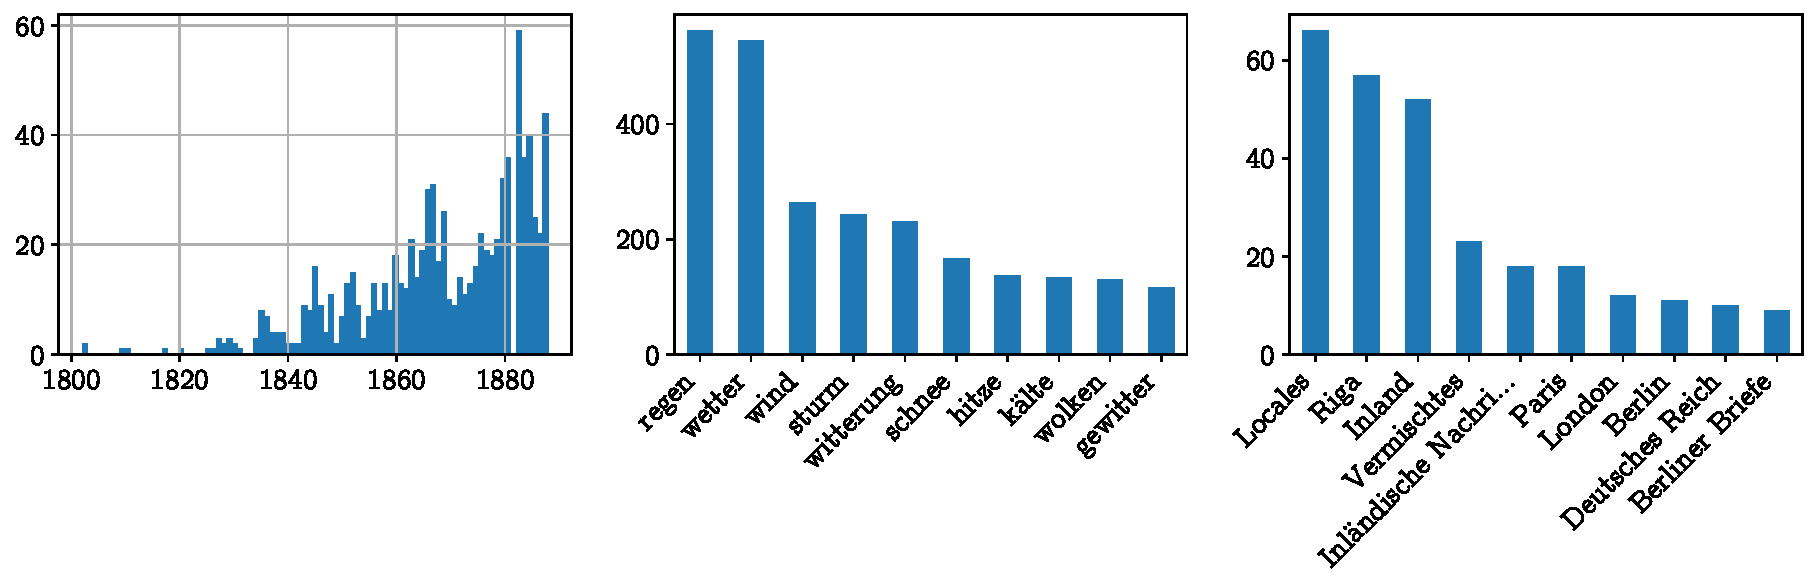
\includegraphics[width=\textwidth]{images/topic_charts_3.pdf}
\end{figure}

\begin{flushleft}
\textbf{Taille :} 858 segments

\textbf{Mots caractéristiques :} \texttt{publicum}, \texttt{musik}, \texttt{gaste}, \texttt{theater}, \texttt{trotz}, \texttt{herrn}, \texttt{sanger}, \texttt{feier}, \texttt{damen}, \texttt{beifall}, \texttt{publicums}, \texttt{concert}, \texttt{besuch}, \texttt{illumination}, \texttt{versammelt}, \texttt{genuß}, \texttt{schonen}, \texttt{besucht}, \texttt{locales}, \texttt{platz}, \texttt{festlich}, \texttt{feuerwerk}, \texttt{concerte}, \texttt{vergnugen}, \texttt{zuschauer}, \texttt{programm}, \texttt{capelle}, \texttt{eindruck}, \texttt{herren}, \texttt{saal}.
\end{flushleft}

\noindent Ce sujet reflète l'importance de la météo pour les événements publics. En effet, de nombreux rassemblements, festivités, défilés, foires, etc. se déroulant en plein air, leur succès dépendait fortement des conditions météorologiques. Les mots les plus caractéristiques de ce thème sont donc \textit{public}, \textit{musique} \textit{invités}, \textit{théâtre}, \textit{visite}, \textit{feu d'artifice}, \textit{programme} et \textit{malgré}, ce dernier indiquant les événements qui se sont déroulés par mauvais temps. Ces types de descriptions provenaient principalement du niveau local (\textit{Locales}, \textit{Riga}, \textit{Inland}), mais parfois des événements plus importants de l'étranger (\textit{Paris}, \textit{Londres}, \textit{Berlin}) étaient également rapportés.

\medskip

\noindent \textbf{Exemple :} \textit{Le jardin impérial a fait une triste expérience cet été. Si une entreprise quelconque y était annoncée, dont on pouvait espérer une plus grande affluence de visiteurs, on pouvait supposer avec quasi-certitude que cette soirée serait pluvieuse, et la pluie peut faire le désespoir des propriétaires d'établissements de jardin. Il est d'autant plus réjouissant que la pluie ait épargné hier soir les illuminations et les feux d'artifice organisés dans le jardin impérial. Un public assez nombreux s'était donc réuni hier sous les vieux arbres feuillus ombragés du jardin. Le feu d'artifice était très beau ; l'étang, dans lequel se reflétaient des centaines de lampions multicolores, offrait un spectacle encore plus beau.}\footnote{RZ 07/07/1888 (\texttt{id: 287414})}

\clearpage

\subsection{Commerce} \label{topic4_commerce}

\begin{figure}[H]
\centering
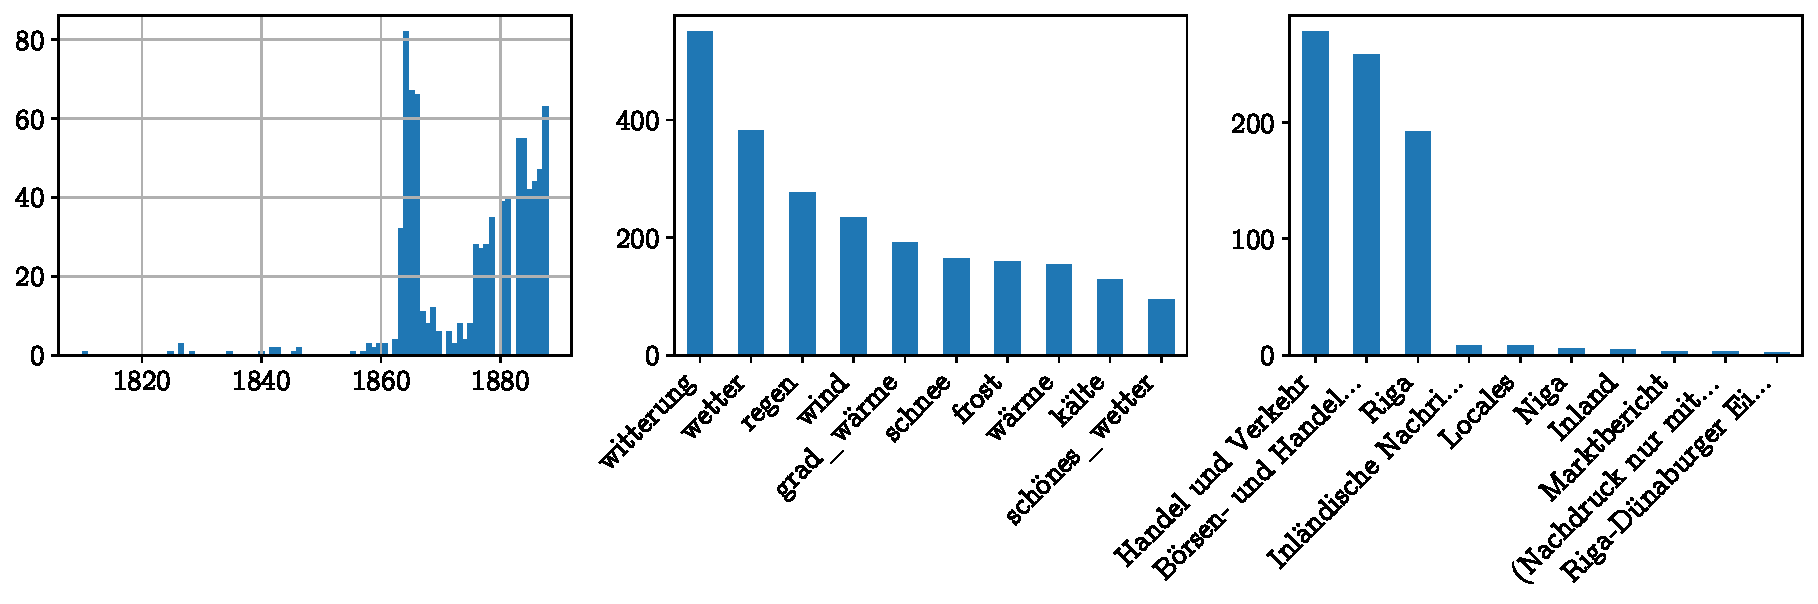
\includegraphics[width=\textwidth]{images/topic_charts_4.pdf}
\end{figure}

\begin{flushleft}
\textbf{Taille :} 848 segments

\textbf{Mots caractéristiques :} \texttt{umsatze}, \texttt{kauflust}, \texttt{bedang}, \texttt{umsatz}, \texttt{roggen\_basis}, \texttt{gedorrte}, \texttt{lieferung}, \texttt{notirungen}, \texttt{handel\_verkehr}, \texttt{umsatzen}, \texttt{loco}, \texttt{geschaft}, \texttt{hafer}, \texttt{abgeber}, \texttt{preise}, \texttt{unverandert}, \texttt{waare}, \texttt{nominell}, \texttt{kleinigkeiten}, \texttt{verkaufer}, \texttt{stimmung}, \texttt{flauer}, \texttt{roggen}, \texttt{preisen}, \texttt{ungedorrter}, \texttt{bengal}, \texttt{zufuhr}, \texttt{borsen\_handels}, \texttt{middling\_fair}, \texttt{angeboten}.
\end{flushleft}

\noindent Ce sujet est fréquent en nombre, mais apparaît dans un ensemble de textes très spécifiques. La quasi-totalité des occurrences sont contenues dans trois types d'articles (\textit{commerce et transport}, \textit{nouvelles boursières et commercials} et \textit{Riga}) et se concentrent sur deux périodes assez courtes qui correspondent à la publication des deux premières de ces rubriques dans le \textit{Rigasche Zeitung}. Le contexte de ces rapports de routine est caractérisé par des mots comme \textit{chiffres d'affaires}, \textit{envie d'achat}, \textit{livraison}, \textit{affaires}, \textit{avoine}, \textit{prix}, \textit{marchandises}, etc. Comme on le voit dans l'exemple, les informations sur les prix du commerce dans le port étaient souvent liées à une brève notice sur les conditions météorologiques (on remarque que les deux mots-clés les plus fréquents sont juste météo et conditions météorologiques).

\medskip

\noindent \textbf{Exemple :} \textit{Commerce et transports. Riga, en Finlande. 14 juin. Ces derniers jours, le temps a été variable, parfois assez frais. Le thermomètre a oscillé entre 8 et 16 degrés de chaleur. Vent de sud-ouest. L'ambiance morose se poursuit sur notre marché des céréales. Le seigle sur la base de 120 livres hollandaises s'est fait à 79 kop. par poud et ce prix serait encore à conditionner. L'avoine est faible et ne se vend pas. La marchandise séchée est proposée à 70 kop. par poud. L'orge séchée livonaise de 100 livres est vendue à 84 kop. le poud. Les graines de lin battues ne sont pas vendues en raison du manque d'offre. Quelques wagons de graines de steppe ont été vendus à 172-173 1/3 kop. le poud, ce qui a permis d'écouler les stocks. Il n'y a pas eu de nouvelles ventes de graines de chanvre. En tout, 600 bateaux sont arrivés, dont 530 en provenance de ports étrangers et 11 de ports finlandais, et 533 sont partis.}\footnote{RZ 14/06/1886 (\texttt{id: 277462})}



\subsection{Navigation} \label{topic6_navigation}

\begin{figure}[H]
\centering
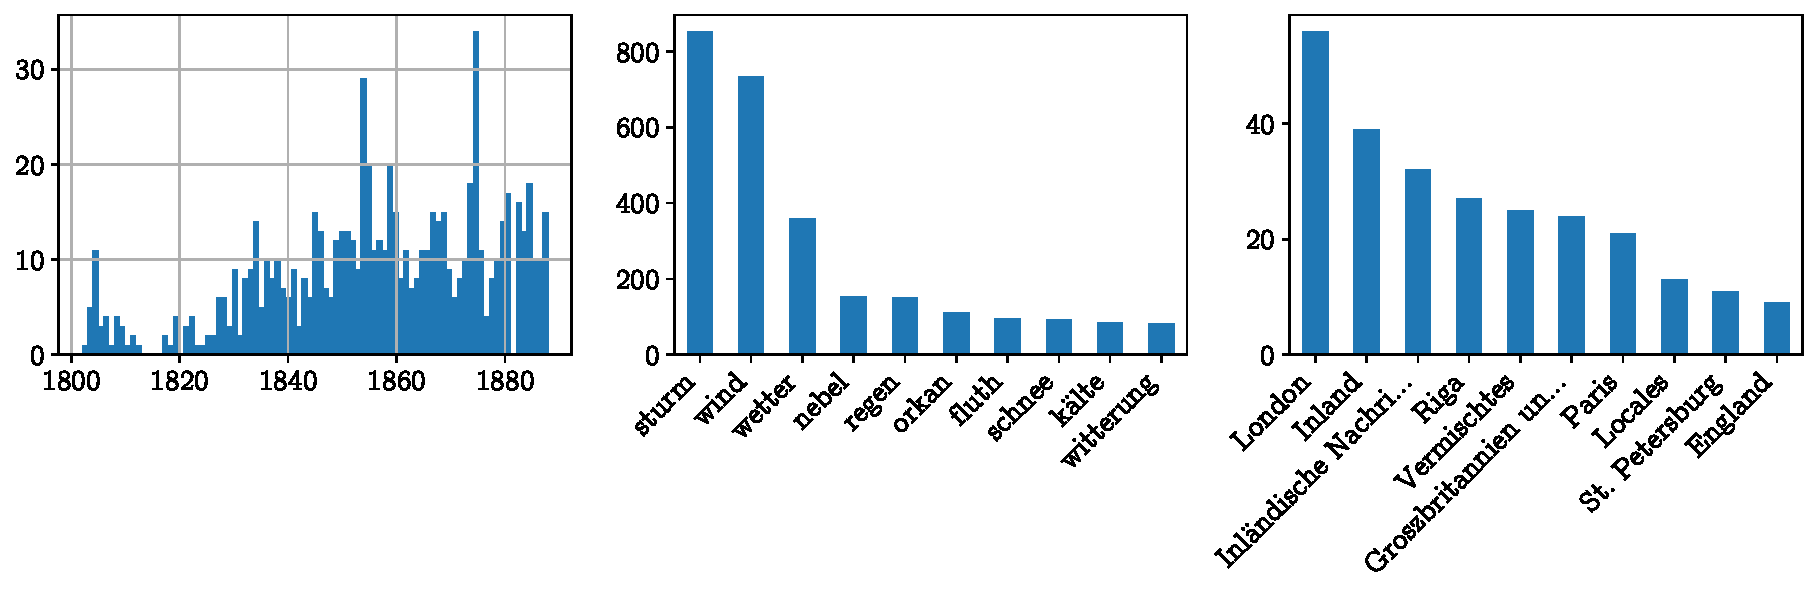
\includegraphics[width=\textwidth]{images/topic_charts_6.pdf}
\end{figure}

\begin{flushleft}
\textbf{Taille :} 734 segments

\textbf{Mots caractéristiques :} \texttt{schiff}, \texttt{schiffe}, \texttt{mannschaft}, \texttt{bord}, \texttt{anker}, \texttt{capitain}, \texttt{dampfer}, \texttt{segel}, \texttt{hafen}, \texttt{fahrzeuge}, \texttt{kuste}, \texttt{strand}, \texttt{segeln}, \texttt{ladung}, \texttt{schiffes}, \texttt{fahrzeug}, \texttt{matrosen}, \texttt{brigg}, \texttt{schiffen}, \texttt{fahrt}, \texttt{rhede}, \texttt{leck}, \texttt{wellen}, \texttt{boote}, \texttt{admiral}, \texttt{besatzung}, \texttt{dampfschiff}, \texttt{bemannung}, \texttt{deck}, \texttt{boot}.
\end{flushleft}

\noindent Ce thème est constitué de rapports sur la navigation, ou plutôt sur ses périls. Des mots comme \textit{navire}, \textit{équipage}, \textit{ancre}, \textit{capitaine}, \textit{bateau à vapeur}, \textit{port}, etc. sont révélateurs de reportages narratifs, dont une part importante concerne des naufrages ou des accidents de mer (\textit{tempête} étant le mot-clé le plus courant). La popularité de \textit{Londres} dans les titres est due à sa centralité dans l'économie maritime du 19ème siècle - de nombreuses nouvelles du monde entier étaient reflétées dans les journaux londoniens. La nature souvent détaillée de ces rapports laisse penser que les lecteurs ont pu apprécier les sensations fortes de ces récits.

\medskip

\noindent \textbf{Exemple :} \textit{Pernau, le 9 octobre. Le 3 du mois dernier, la tempête de sud-sud-est a arraché de ses ancres le bateau-lanterne \og Julie Louise \fg{} appartenant à la maison de commerce locale Jacob Jacke \& Comp. et l'a fait dériver sur la plage à environ 4 milles de la ville. Pendant la nuit qui suivit, par une tempête orageuse et un niveau d'eau élevé (6 pieds au-dessus du niveau ordinaire), le bateau s'était couché sur le côté, et le marin et un matelot qui étaient restés sur le bateau étaient restés assis sur le mât qui dépassait de quelques brasses au-dessus de l'eau, de 10 heures du soir à 10 heures du matin le lendemain. Quatre pêcheurs tentèrent un sauvetage, mais leur bateau fut renversé par la violence des vagues, et l'un d'eux se noya à cette occasion. Les trois autres pêcheurs, ainsi que les deux personnes qui se trouvaient sur le mât, furent sauvés par plusieurs lotisseurs et matelots, au péril de leur vie.}\footnote{RZ 21/10/1843 (\texttt{id: 72189})}

\clearpage


\subsection{Hiver-ferroviaire} \label{topic8_hiver-ferroviaire}

\begin{figure}[H]
\centering
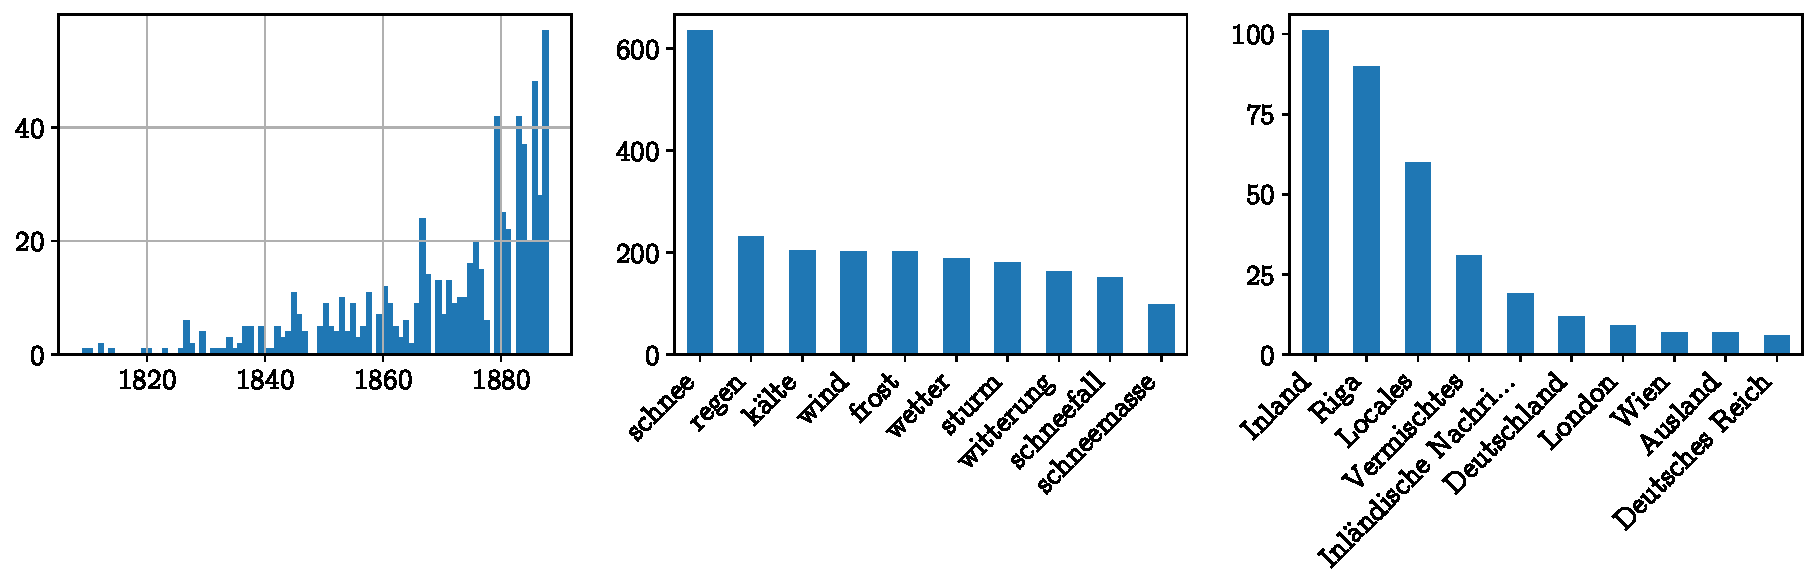
\includegraphics[width=\textwidth]{images/topic_charts_8.pdf}
\end{figure}

\begin{flushleft}
\textbf{Taille :} 677 segments

\textbf{Mots caractéristiques :} \texttt{verkehr}, \texttt{reinigung}, \texttt{strecke}, \texttt{schneemassen}, \texttt{eingestellt}, \texttt{stecken}, \texttt{zuge}, \texttt{eingesandt}, \texttt{arbeiter}, \texttt{verspatung}, \texttt{schneefall}, \texttt{straßen}, \texttt{schneemaffen}, \texttt{post}, \texttt{schneewehen}, \texttt{polizei}, \texttt{thauwetter}, \texttt{abgelassen}, \texttt{schnee}, \texttt{dirschau}, \texttt{unmoglich}, \texttt{locales}, \texttt{bahnen}, \texttt{bahn}, \texttt{communication}, \texttt{hochwasser}, \texttt{eintritt}, \texttt{locomotiven}, \texttt{schneesturme}, \texttt{waggon}.
\end{flushleft}

\noindent Ce thème comprend des nouvelles sur les conditions hivernales sévères, mais il est surtout dominé par un seul type d'information : les perturbations des communications causées par la neige (comme le montrent les mots \textit{trafic}, \textit{train}, \textit{retard}, \textit{masse de neige}, \textit{travailleurs}, \textit{poste}, \textit{routes}). Ceci est également illustré par la distribution temporelle du sujet, qui connaît une forte augmentation dans les années 1880. L'exemple ci-dessous illustre comment les nouveaux moyens de transport et de communication, plus avancés, étaient aussi plus sensibles aux caprices du climat.

\medskip

\noindent \textbf{Exemple :} \textit{Aujourd'hui encore, nous n'avons reçu que les journaux autrichiens ; tout le reste du courrier étranger a encore manqué aujourd'hui, tant le matin qu'à midi, de sorte qu'il manque maintenant cinq ou six postes étrangers. Ce que nous publions aujourd'hui sous la rubrique \og étranger \fg{} est entièrement tiré de journaux autrichiens. D'autres villes se plaignent également des perturbations du trafic ferroviaire dues aux congères et autres phénomènes naturels. Le \og Tages.-Anz. für Libau \fg{} écrit dans son numéro d'hier : \og Entre les stations de Sehaulen, Koschedary et Dünabürg, des chutes de neige colossales ont eu lieu, ce qui a perturbé le service pendant un certain temps. Sur le chemin de fer de Varsovie, l'accumulation de neige a également entraîné des irrégularités dans le trafic \fg{}}.\footnote{RZ 10/03/1888 (\texttt{id: 285886})}




\subsection{Inondation} \label{topic9_inondation}

\begin{figure}[H]
\centering
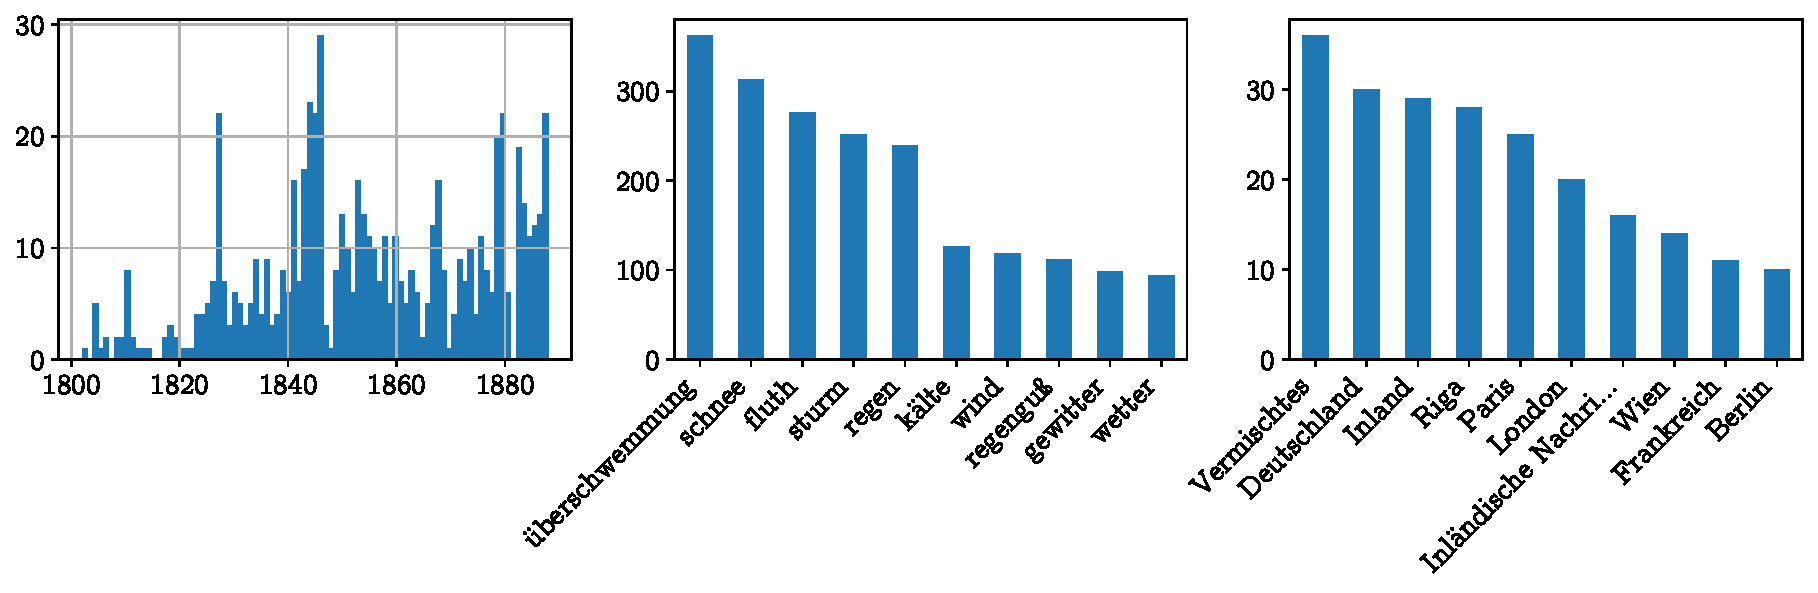
\includegraphics[width=\textwidth]{images/topic_charts_9.pdf}
\end{figure}

\begin{flushleft}
\textbf{Taille :} 657 segments

\textbf{Mots caractéristiques :} \texttt{uberschwemmt}, \texttt{uberschwemmung}, \texttt{brucken}, \texttt{ueberschwemmung}, \texttt{eingesturzt}, \texttt{weggerissen}, \texttt{fluthen}, \texttt{ortschaften}, \texttt{hauser}, \texttt{angerichtet}, \texttt{zerstort}, \texttt{fortgerissen}, \texttt{einwohner}, \texttt{menschenleben}, \texttt{straßen}, \texttt{wasser}, \texttt{heimgesucht}, \texttt{umgekommen}, \texttt{verheerungen}, \texttt{wohnungen}, \texttt{mehrere}, \texttt{verwustet}, \texttt{ungluck}, \texttt{einsturz}, \texttt{angeschwollen}, \texttt{stadt}, \texttt{uberschwemmten}, \texttt{wolkenbruch}, \texttt{unglucklichen}, \texttt{weggeschwemmt}.
\end{flushleft}

\noindent Ce sujet-ci relaie l'actualité des inondations et des dégâts qui en résultent, tant en Europe qu'au niveau local. (titres \textit{Allemagne}, \textit{affaires domestiques}, \textit{Riga}, \textit{Paris}, \textit{Londres}, etc). Les mots caractéristiques indiquent les dommages causés aux maisons, aux fermes et aux infrastructures (\textit{effondrés}, \textit{emportés}, \textit{maisons}, \textit{ponts}, \textit{habitants}, \textit{vies humaines}, \textit{détruits}, \textit{réduits en poussière}, etc.). Il est intéressant de noter que ce sujet est réparti plus uniformément dans le temps, avec le plus grand nombre de segments dans les années 1840. Ce fait sera analysé dans la section \ref{comparison}. Il s'avère également que un nombre de segments regroupés sous ce sujet-ci se traitent en fait des avalanches - probablement à cause des descriptions similaires par rapport aux dommages. Cependant, la partie sur les avalanches ne comporte que 19\% des segments de ce sujet.

\medskip

\noindent \textbf{Exemple :} \textit{Lors de l'orage du 28 mai dans la région de Gladenbach, l'eau était si haute dans la localité d'Erdhausen que les personnes n'ont pu être sauvées du deuxième étage qu'au péril de leur vie. Le 1er juin, dans la région de Sauerschwabenheim, à quatre heures de Gladenbach, dans le Grand-Duché de Hesse, un terrible orage, accompagné d'une pluie torrentielle, a causé de grands ravages. Les éléments dévastateurs auraient arraché des granges, emporté le bétail hors des champs et inondé les vignes et les champs de céréales.}\footnote{RZ 08/06/1826 (\texttt{id: 31772})}

\clearpage



\subsection{Télégrammes} \label{topic10_télégrammes}

\begin{figure}[H]
\centering
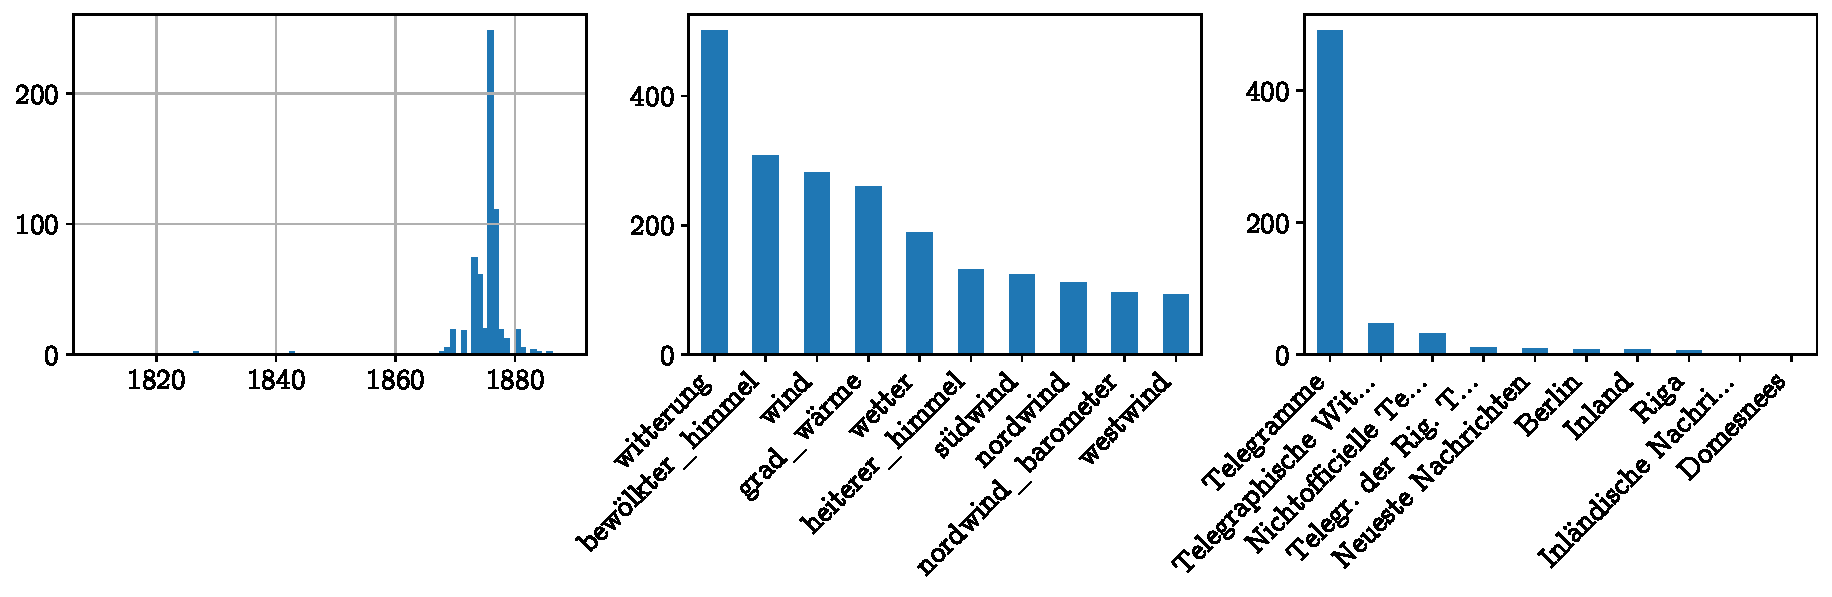
\includegraphics[width=\textwidth]{images/topic_charts_10.pdf}
\end{figure}

\begin{flushleft}
\textbf{Taille :} 640 segments

\textbf{Mots caractéristiques :} \texttt{kiew\_odessa}, \texttt{moskau\_kasan}, \texttt{grad\_archangel}, \texttt{morqens}, \texttt{uleaborg\_mill}, \texttt{petersburg}, \texttt{schwarzen\_meere}, \texttt{uleaborg}, \texttt{barometrisches}, \texttt{schwacher}, \texttt{wilna}, \texttt{weht}, \texttt{windau\_wilna}, \texttt{barometrische}, \texttt{minimum}, \texttt{belgien}, \texttt{morgens\_maßiger}, \texttt{luftdruckes}, \texttt{heiterer\_himmel}, \texttt{kuopio}, \texttt{außert}, \texttt{rußland}, \texttt{kill}, \texttt{domesnees}, \texttt{telegramm}, \texttt{archangel}, \texttt{varometer}, \texttt{maßiger}, \texttt{unbestandig}, \texttt{luftdruck}.
\end{flushleft}

\noindent Ce sujet est entièrement constitué de télégrammes météorologiques, un type de texte répétitif concentré dans une petite fenêtre temporelle. Pendant quelques années notamment, les télégrammes de l'observatoire météorologique de Saint-Pétersbourg ont été imprimés dans le Rigasche Zeitung. Pour des raisons d'espace, je n'ai pas inclus dans l'exemple ci-dessous une liste d'environ 10 villes de l'empire russe et les pressions atmosphériques et températures correspondantes, qui est en fait l'élément principal de ce sujet, faisant de ces noms de lieux certains des mots les plus caractéristiques du sujet (\textit{Kiev}, \textit{Moscou}, \textit{Kasan}, \textit{Mer Noire}, \textit{Vilnius} etc.)

\medskip

\noindent \textbf{Exemple :} \textit{Domesnees, le 11 mars, 9 h du matin. Vent faible du nord-ouest, baromètre le 10 mars, 9 h du soir, 29-1, le 11 mars, 9 h du matin, 29-2. Thermomètre 1 degré de gelée, ciel nuageux. Le niveau de la glace n'a pas changé. Pétersbourg, le 11 mars. (Télégramme de l'Observatoire central de physique à la station météorologique de l'Association des naturalistes à Riga). Le minimum barométrique s'est déplacé vers le lac Onega. Sur la mer Baltique et la mer Noire, le vent est faible. Dans le nord de la Russie, il neige. Au sud, le temps s'est éclairci.}\footnote{RZ 12/03/1876 (\texttt{id: 227867})}

\clearpage


\subsection{Tempête-grêle} \label{topic12_tempête-grêle}

\begin{figure}[H]
\centering
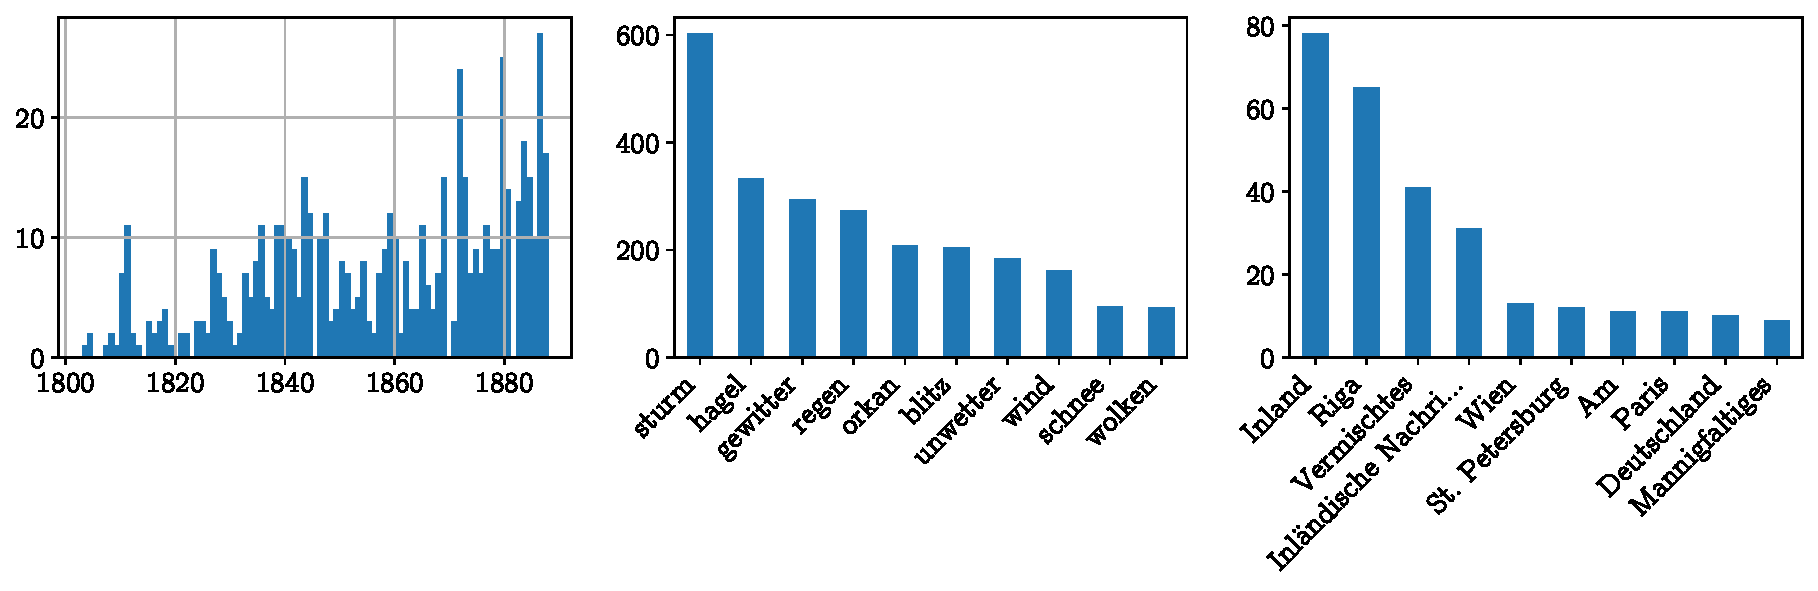
\includegraphics[width=\textwidth]{images/topic_charts_12.pdf}
\end{figure}

\begin{flushleft}
\textbf{Taille :} 591 segments

\textbf{Mots caractéristiques :} \texttt{dacher}, \texttt{entwurzelt}, \texttt{hagel}, \texttt{abgedeckt}, \texttt{angerichtet}, \texttt{orkan}, \texttt{erschlagen}, \texttt{unwetter}, \texttt{fensterscheiben}, \texttt{zerstort}, \texttt{beschadigt}, \texttt{umgeworfen}, \texttt{baume}, \texttt{zertrummert}, \texttt{verwustungen}, \texttt{gebaude}, \texttt{heimgesucht}, \texttt{schaden}, \texttt{hauser}, \texttt{vernichtet}, \texttt{umgegend}, \texttt{umgesturzt}, \texttt{gewuthet}, \texttt{mehrere}, \texttt{gerissen}, \texttt{verwustet}, \texttt{wuthete}, \texttt{anrichtete}, \texttt{windhose}, \texttt{abgerissen}.
\end{flushleft}

\noindent Ce thème est clairement dominé par les nouvelles concernant les dommages causés par les tempêtes, dont les tempêtes de grêle sont les plus importantes. Les descriptions des dommages causés aux bâtiments, aux champs, aux jardins, etc. sont un élément important (\textit{toitures}, \textit{déracinées}, \textit{abattues}, \textit{intempéries}, \textit{vitres}, etc.). Les mots-clés climatiques les plus courants sont tempête, grêle, tonnerre, pluie, etc., et la plupart des segments se trouvent sous les titres Intérieur et Riga. Voir aussi la page \pageref{about:hagel}.

\medskip

\noindent \textbf{Exemple :} \textit{Alexin (Gouvernement de Tula), du 17 juillet. Le 17 juin, à 3 heures de l'après-midi, notre ville a subi, lors de la rencontre de deux nuages orageux, de violents éclairs, du tonnerre, des tempêtes, de la pluie et de la grêle, des dommages importants causés par cette dernière, qui a duré une heure entière,} [les grêlons étaient] \textit{de la taille d'un œuf de pigeon, de poule et même d'oie, et qui a brisé les fenêtres des 5 églises locales, des locaux des autorités et de toutes les maisons. L'ouragan a arraché le toit en fer de l'église de Nikolaev, ainsi que les toits de plusieurs maisons, et en a détruit d'autres. Le toit en fer de la grande maison en pierre des marchands de la première guilde et des fabricants de Maßlow fut arraché et projeté à une demi-lieue de la maison. Les jardins fruitiers, les légumes de toutes sortes et même l'herbe ont été brisés par la grêle ; dans les environs de la ville, le seigle a été complètement détruit dans les champs sur lesquels l'orage est passé, et les paysans ont subi une perte considérable. Les grêlons pesaient jusqu'à 34 Lot} [1 lb].\footnote{RZ 17/08/1826 (\texttt{id: 31978})}

\clearpage


\subsection{Science} \label{topic13_science}

\begin{figure}[H]
\centering
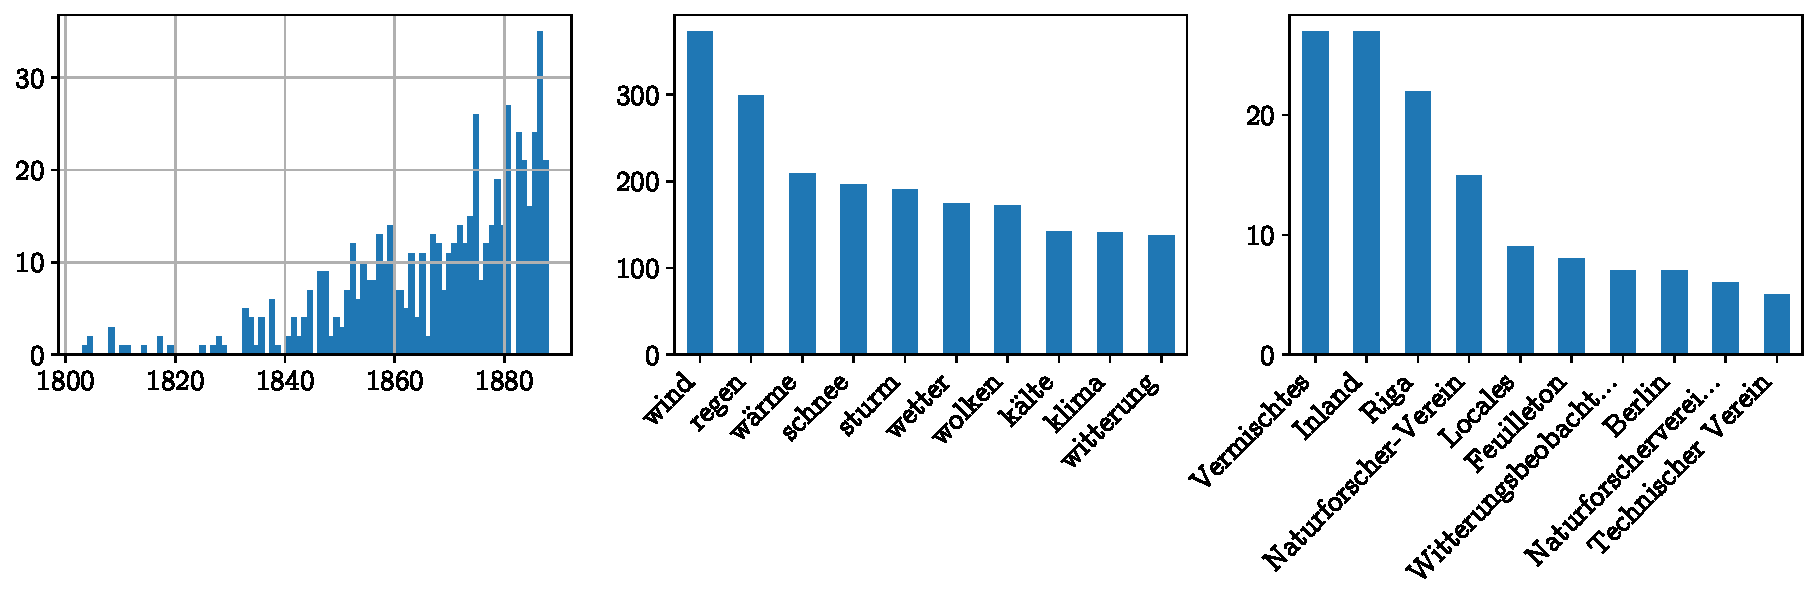
\includegraphics[width=\textwidth]{images/topic_charts_13.pdf}
\end{figure}

\begin{flushleft}
\textbf{Taille :} 576 segments

\textbf{Mots caractéristiques :} \texttt{beobachtungen}, \texttt{erscheinungen}, \texttt{erscheinung}, \texttt{beobachtet}, \texttt{erdoberflache}, \texttt{temperatur}, \texttt{ursachen}, \texttt{oberflache}, \texttt{atmosphare}, \texttt{beobachtung}, \texttt{sonne}, \texttt{beobachter}, \texttt{stromungen}, \texttt{planeten}, \texttt{atmospharischen}, \texttt{untersuchungen}, \texttt{zusammenhang}, \texttt{aequator}, \texttt{theorie}, \texttt{perioden}, \texttt{beziehung}, \texttt{niederschlage}, \texttt{einfluß}, \texttt{professor}, \texttt{periode}, \texttt{vortragende}, \texttt{meteorologie}, \texttt{erde}, \texttt{schwankungen}, \texttt{entstehen}.
\end{flushleft}

\noindent Caractérisé par des termes plus généraux et scientifiques (\textit{observations}, \textit{phénomènes}, \textit{causes}, \textit{atmosphère}, \textit{courants}, \textit{théorie}, \textit{professeur}, \textit{météorologie}), ce thème contient des textes qui analysent le climat et la nature de manière empirique. Notamment, les différents mots-clés sont représentés de manière assez égale dans le thème, et de nombreux segments se retrouvent dans les rapports de l'Association des naturalistes de Riga.

\medskip

\noindent \textbf{Exemple :} \textit{Glasenapp présente ici les résultats d'études sur la salinité de l'eau de la mer Baltique qu'il a effectuées en été 1876 à Bilderlingshof. Notre plage doit notamment aux vents dominants du nord-ouest le fait que, malgré la proximité de l'embouchure de Düna} [Daugava], \textit{la salinité de l'eau de mer y est presque aussi élevée que sur l'île d'Oesel, par exemple. En revanche, lorsque le vent souffle en sens inverse, l'eau de la dune est poussée vers les plages, ce qui réduit la salinité. Afin de clarifier cette relation, Redner mesura pendant 51 jours la salinité de l'eau et nota en même temps la direction et la force du vent, ainsi que la température de l'eau et de l'air. Les résultats de ces observations et de ces mesures ont été reportés par l'orateur sous forme graphique, la salinité, les températures et le niveau de l'eau étant représentés par des courbes, la direction et la force du vent par des flèches de direction et de longueur correspondantes.
Ce dessin, présenté à l'assemblée, montre clairement la relation entre la salinité et le vent, même s'il y a bien sûr des irrégularités et des écarts.}\footnote{RZ 29/04/1878 (\texttt{id: 240569})}

\clearpage


\subsection{Düna} \label{topic14_düna}

\begin{figure}[H]
\centering
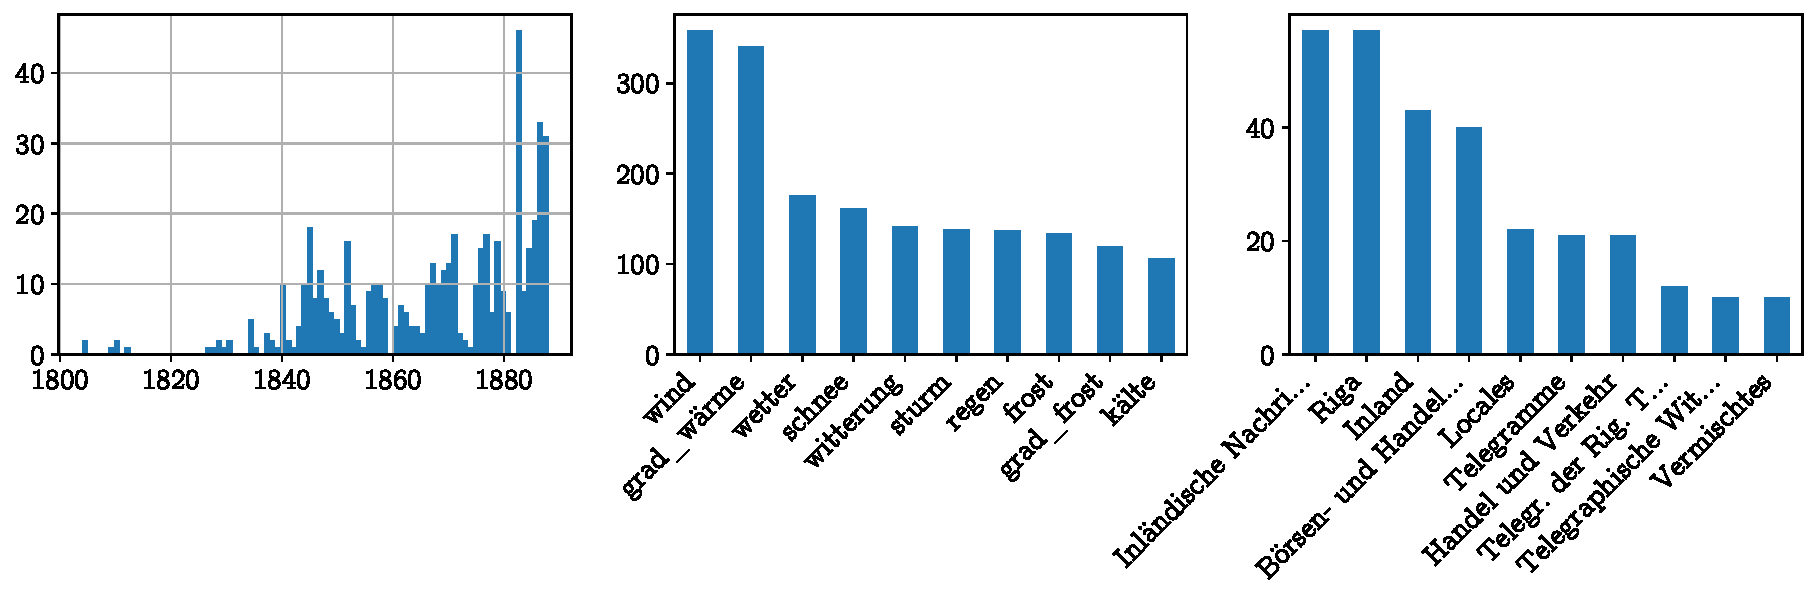
\includegraphics[width=\textwidth]{images/topic_charts_14.pdf}
\end{figure}

\begin{flushleft}
\textbf{Taille :} 516 segments

\textbf{Mots caractéristiques :} \texttt{eisfrei}, \texttt{bolderaa}, \texttt{duna}, \texttt{muhlgraben}, \texttt{eisgang}, \texttt{eisdecke}, \texttt{kreutzburg}, \texttt{fahrwasser}, \texttt{wasserstand}, \texttt{grad\_warme}, \texttt{grad\_frost}, \texttt{seegatt}, \texttt{marz}, \texttt{normal}, \texttt{passage}, \texttt{romershof}, \texttt{gestern}, \texttt{nachm}, \texttt{oger}, \texttt{morgens}, \texttt{offenes\_wasser}, \texttt{abgetrieben}, \texttt{eisstand}, \texttt{flußmundung}, \texttt{vorm}, \texttt{domesnees}, \texttt{abstromung}, \texttt{stintsee}, \texttt{rhede}, \texttt{eise}.
\end{flushleft}

\noindent Ce sujet est probablement le plus spécifique à Riga. Il s'agit d'informations sur la navigation sur la rivière Düna (Daugava) qui traverse Riga et se jette dans la mer Baltique, étant le corridor de transport le plus important de toute la région (comme le montrent les mots-clés \textit{Bolderaa}, \textit{Düna}, \textit{embouchure de la rivière}, \textit{chenal}, \textit{passage}, etc.). Ces tranches qui comprennent principalement des informations sur le niveau d'eau et la glace en hiver (\textit{niveau de l'eau}, \textit{embâcle}, \textit{eau libre}, etc.) n'ont pas été publiées exclusivement sous forme de télégrammes, mais aussi plus tôt. Toutefois, le sujet ne devient important qu'à partir des années 1840.

\medskip

\noindent \textbf{Exemple :} \textit{Dünaburg, le 28 février, à 8h 1/4 du matin. Sur les rives, la glace de la Düna s'est rompue en plusieurs endroits. Par ciel clair et vent du nord, il gèle 4 degrés à l'heure. Kreutzburg, 28 février. Le matin à 9 heures. La couche de glace de la Düna est encore solide. 4 degrés de gel. Vent d'ouest.
Römershof. 28 février, matin 8 heures. Niveau de l'eau de la Düna environ 2 pieds et demi au-dessus de la normale, glace épaisse. 3 degrés de gel. Vent du sud-ouest. Oger, 28 février, 8 heures du matin. Niveau d'eau de la Düna normal, couche de glace solide, passage sans encombre. 2 degrés de gel. Vent du sud-ouest. Mühlgraben, 28 février, matin 7 h 1/2. Niveau d'eau normal. La glace de vase est debout. Gelée de 6 degrés, vent d'ouest faible. Dans la nuit, il est tombé environ 2 pouces de neige.}\footnote{RZ 28/02/1887 (\texttt{id: 280738})}

\clearpage


\subsection{Foudre} \label{topic15_foudre}

\begin{figure}[H]
\centering
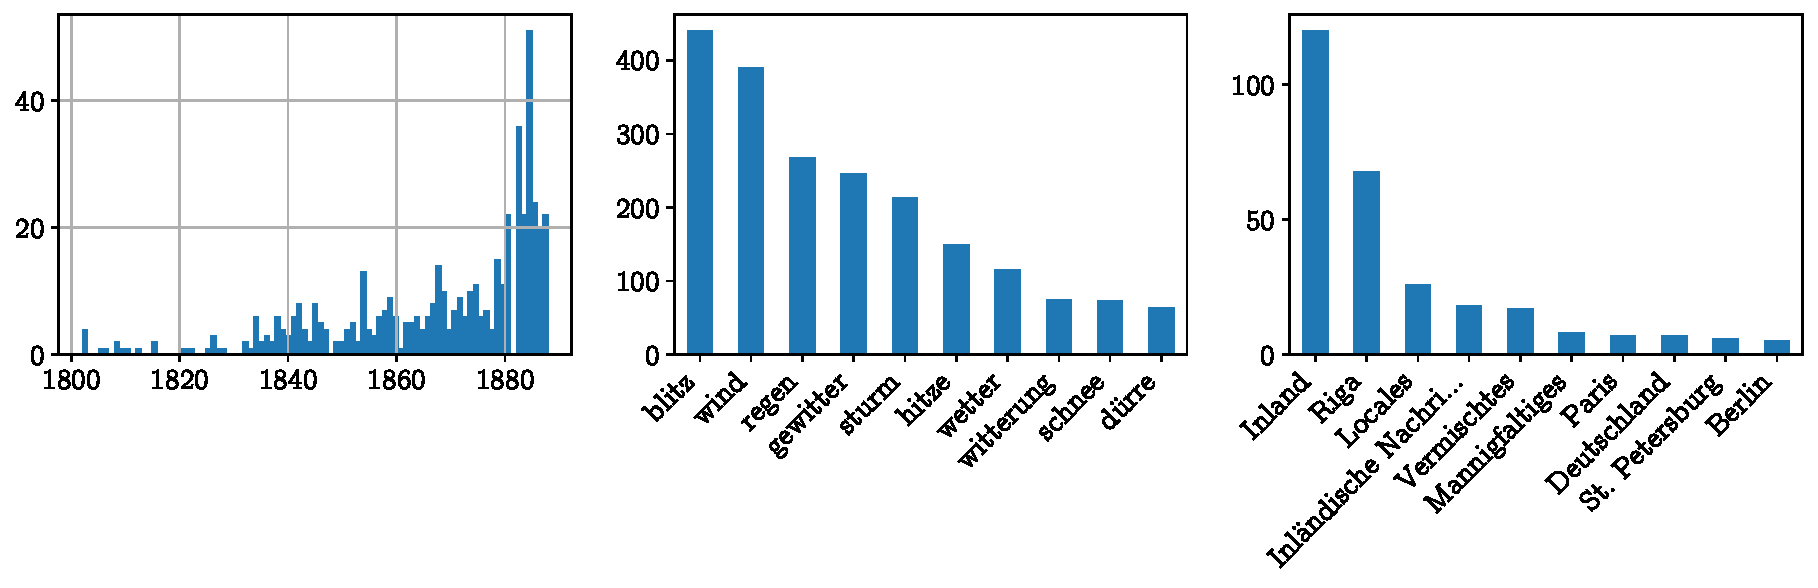
\includegraphics[width=\textwidth]{images/topic_charts_15.pdf}
\end{figure}

\begin{flushleft}
\textbf{Taille :} 497 segments

\textbf{Mots caractéristiques :} \texttt{flammen}, \texttt{feuer}, \texttt{gebaude}, \texttt{raub\_flammen}, \texttt{brand}, \texttt{feuerwehr}, \texttt{hauser}, \texttt{feuersbrunst}, \texttt{brannte}, \texttt{blitz}, \texttt{brande}, \texttt{retten}, \texttt{niedergebrannt}, \texttt{eingeaschert}, \texttt{dach}, \texttt{gesinde}, \texttt{asche\_gelegt}, \texttt{brandstatte}, \texttt{entzundete}, \texttt{brandwunden}, \texttt{haus}, \texttt{feuers}, \texttt{flamme}, \texttt{loschen}, \texttt{hause}, \texttt{schlug}, \texttt{blitzschlag}, \texttt{kirche}, \texttt{spritzen}, \texttt{brannten}.
\end{flushleft}

\noindent Ce sujet s'inscrit dans les actualités plus générales sur les incendies, le lien étant le rôle que joue la foudre dans un nombre de ces incidents (indiqués par les mots \textit{feu}, \textit{bâtiment}, \textit{pompiers}, \textit{sauver}, \textit{réduit en cendres}). Les mots-clés les plus courants sont \textit{foudre}, \textit{vent} (qui peut soit alimenter soit éteindre les flammes) et \textit{pluie}. La plupart de ces nouvelles proviennent du niveau local, mais elles ne connaissent une forte augmentation que dans les années 1880. Une cause possible de ce phénomène pourrait être liée à un certain développement du secteur des assurances, comme le suggère l'exemple ci-dessous.

\medskip

\noindent \textbf{Exemple :} \textit{Le 30 juin, la foudre est tombée sur l'étable à bétail du ménage Dreije à Suhr et l'étable ainsi que trois trèfles ont été la proie des flammes. Le 23 juin, à 7 heures de l'après-midi, la foudre a brûlé une étable et deux granges appartenant à Uljan Allex, propriétaire de la ferme de Bewern, et à 12 heures de la nuit, la foudre a brûlé deux étables et deux granges appartenant à Jahn Tschamann, également à Bewern. Le 2 juillet, la foudre s'est abattue sur l'enclos du gardien de brousse Apscheneek et a brûlé l'enclos. Les dégâts sont estimés à 1000 roubles. Le bâtiment est assuré par l'assurance incendie de Courlande pour 60 Rbl.}\footnote{RZ 11/07/1885 (\texttt{id: 273518})}


\clearpage

\subsection{Comparaison des sujets} \label{comparison}

Les vecteurs correspondantes à chaque document peuvent être visualisés à l'aide d'une projection UMAP, de même manière que sur la figure \ref{fig:keyword_umap}. Ici, les points signifient les segments et ils sont colorés selon le sujet principal auquel ils appartiennent.

\begin{figure}[h]
    \centering
    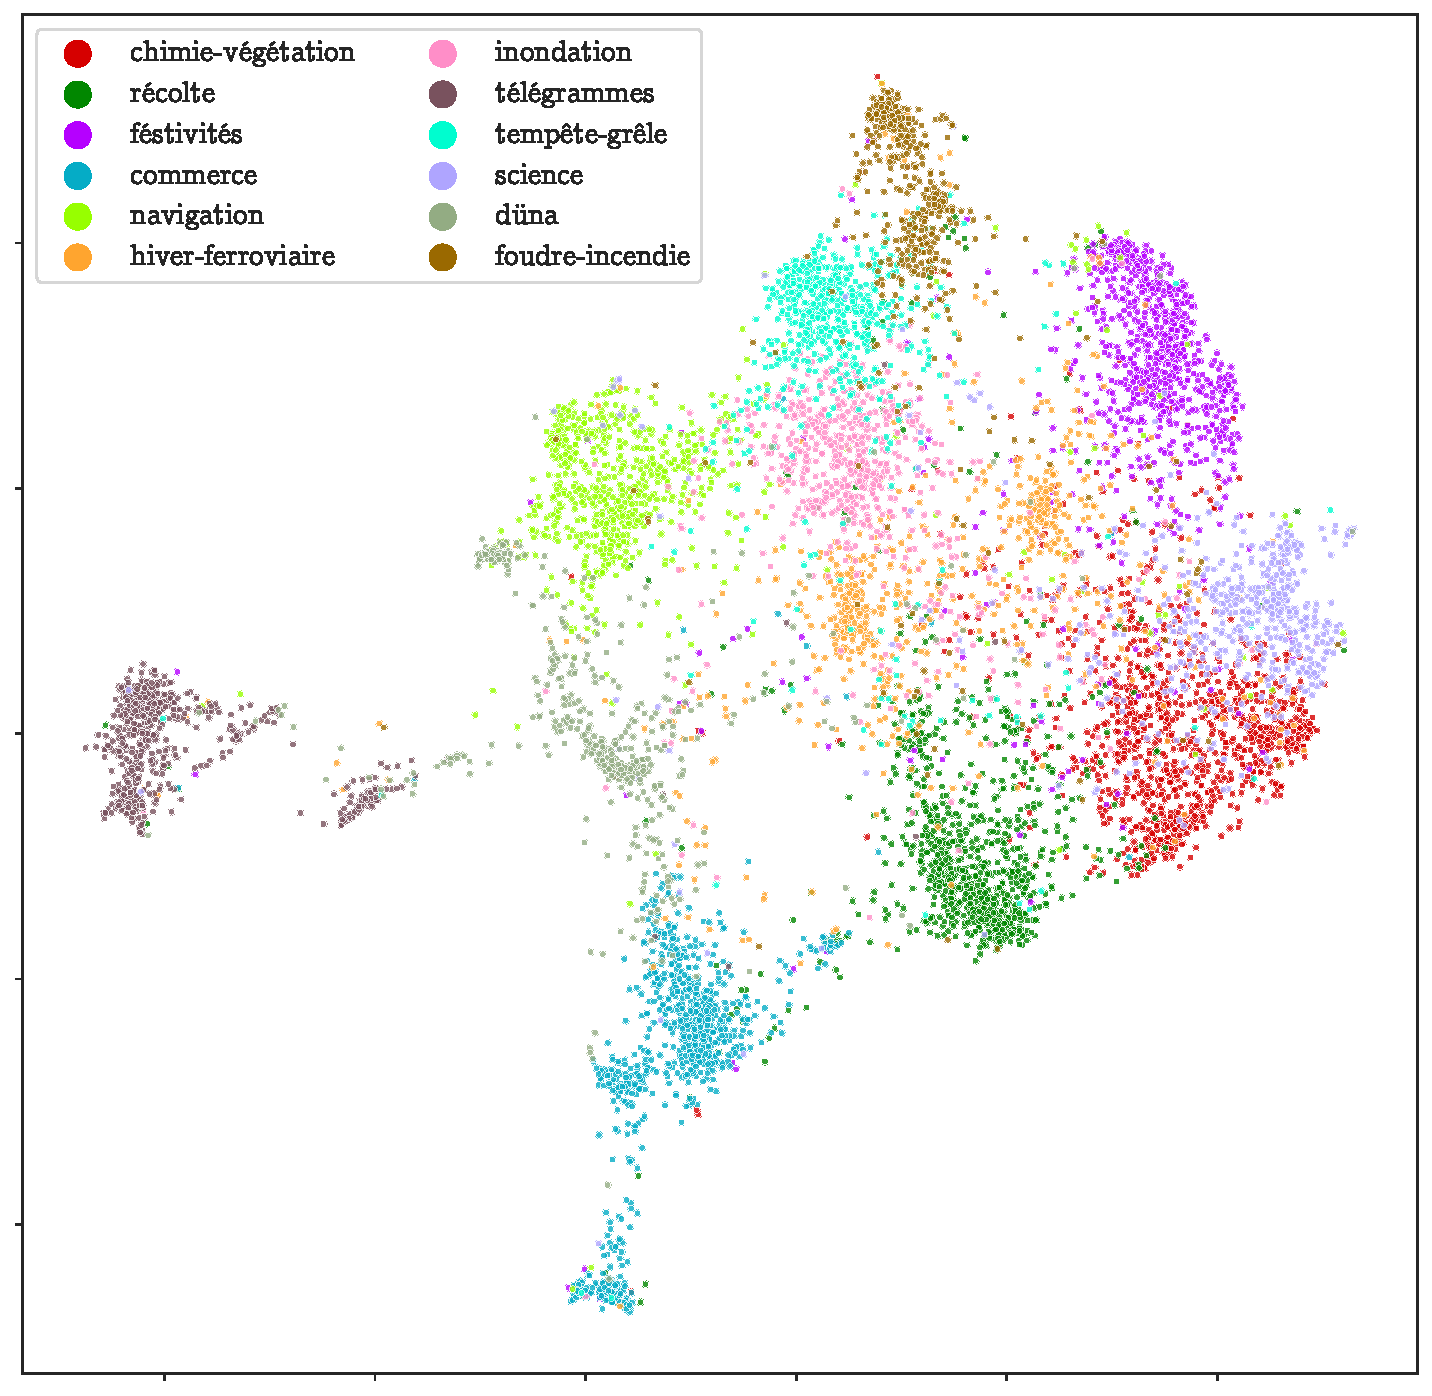
\includegraphics[width=\textwidth]{images/topics_umap.pdf}
    \caption{Visualisation spatiale des sujets}
    \label{fig:topic_umap}
\end{figure}

La visualisation ajoute une autre dimension à l'analyse thématique. Tout d'abord, on peut voir quels sont les sujets qui sont généralement les plus similaires les uns aux autres. Par exemple, les thèmes \textit{foudre-incendie}, \textit{tempête-grêle} et \textit{inondation} sont regroupés dans la partie supérieure de la figure. Tous ces thèmes contiennent principalement des descriptions d'événements singuliers et sont souvent de nature catastrophique, mentionnant des dommages et des victimes. La nature de ces sujets peut être encore mieux illustrée en examinant les 46 sujets originaux qui ont été fusionnés pour obtenir les sujets actuels. Par exemple, le sujet \textit{inondation} est compris de trois sujets originels, dont les mots caractéristiques sont montrés sur la figure \ref{fig:suptopic_worcloud_9}, où la taille des mots correspond à leur importance pour le sujet. Comme mentionné en haut, une partie du sujet \textit{inondation} est en fait compris des textes sur les avalanches (\textit{Lawine}), mais il est également intéressant à noter que le nuage au centre représente un sous-sujet des inondations en France (mots-clés \textit{Lyon}, \textit{Loire}, \textit{Rhône}, \textit{France} et \textit{Moniteur}). En examinant la répartition temporelle de ce sous-sujet, il s'avère que le plus grand nombre de ces textes-là proviennent des années 1846 et 1856, qui correspondent nettement aux graves inondations survenues en France ces années-là.\footnote{France 1846/1856 inondations ref}

\begin{figure}[h]
    \centering
    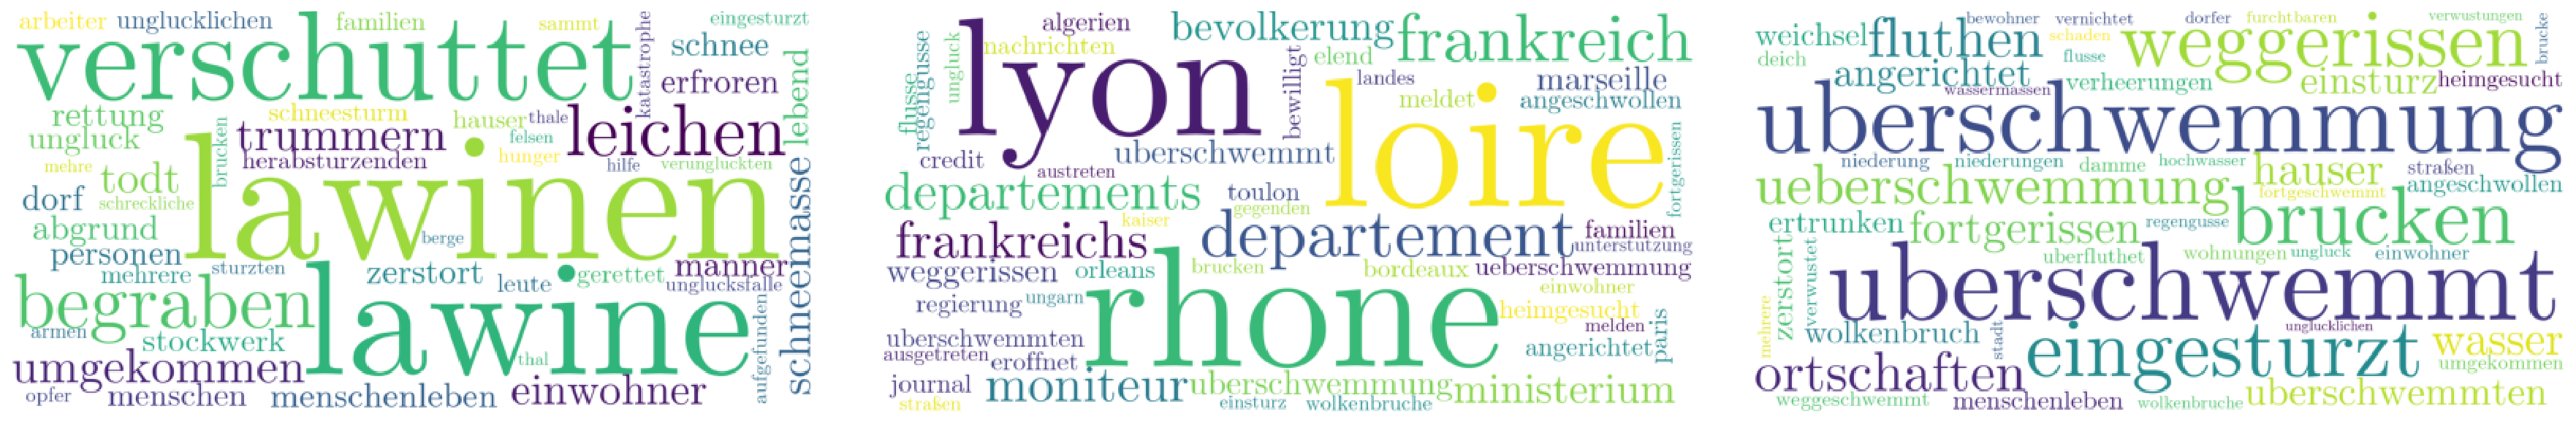
\includegraphics[width=0.9\textwidth]{images/subtopics_wordcloud_9.pdf}
    \caption{Nuages des mots des trois sujets qui composent le sujet \textit{inondation}}
    \label{fig:suptopic_worcloud_9}
\end{figure}


Dans la partie droite du graphique \ref{fig:topic_umap}, le thème \textit{chimie-végétation} présente un chevauchement important avec deux de ses voisins immédiats, \textit{science} et \textit{récolte}, ce qui est conforme à l'analyse présentée à la page \pageref{topic1_chimie-vegetation}. En fait, de nombreux points dans cette zone de chevauchement appartiennent très probablement à deux thèmes dans une mesure presque égale, mais sont colorés par celui qui est légèrement dominant. Cela montre une transition assez douce entre les descriptions scientifiques du climat, truffées d'observations et autres, et les rapports agricoles sur les récoltes, par exemple. Parmi les documents qui comblent ce fossé, on pourrait probablement trouver de nombreux textes similaires à l'exemple 1 présenté à la page \pageref{topic1_chimie-vegetation} - une sorte de genre agricole-économique à l'esprit progressiste dont les prédécesseurs peuvent être trouvés dans la région balte et dans le reste de l'Europe à partir du 17ème siècle.

\begin{figure}[h]
    \centering
    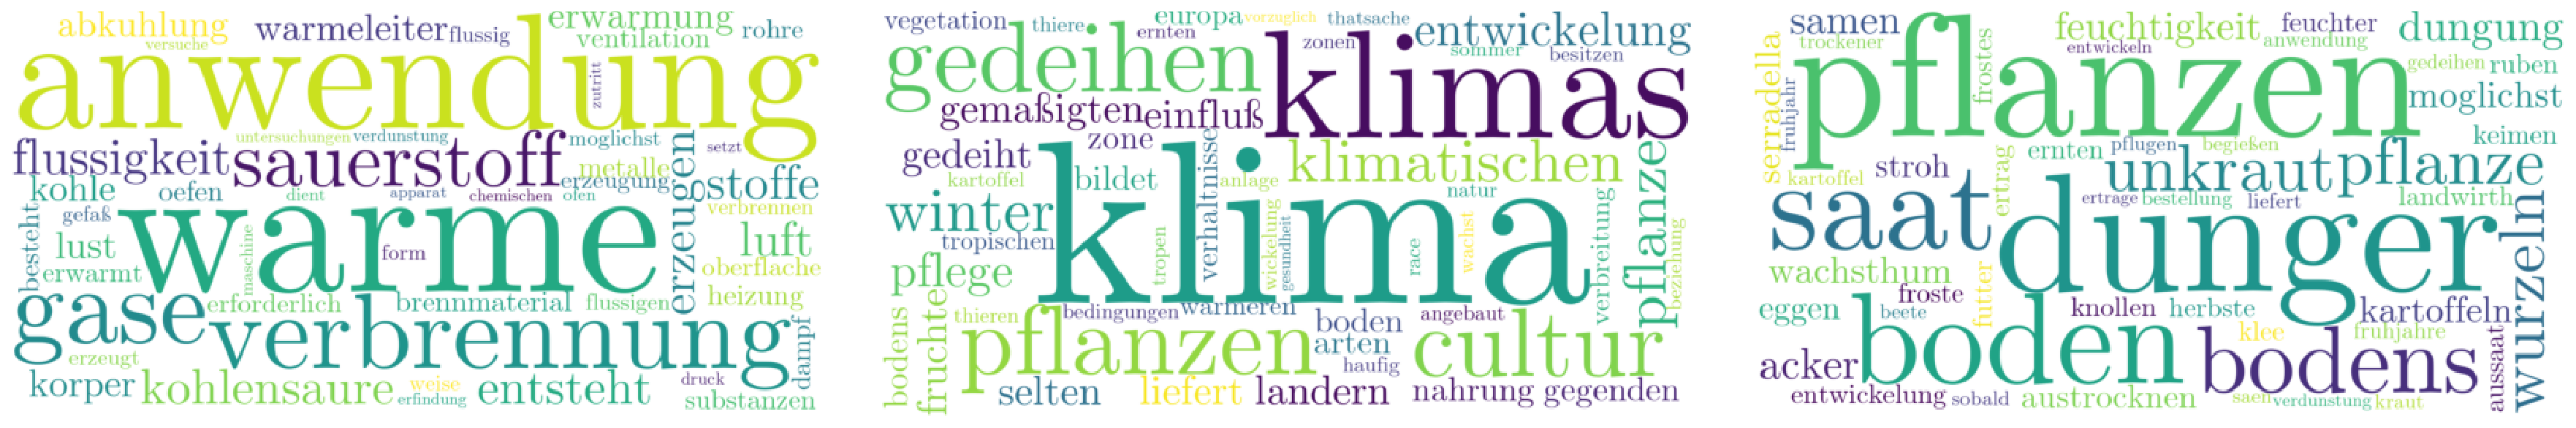
\includegraphics[width=0.9\textwidth]{images/subtopics_wordcloud_1.pdf}
    \caption{Nuages des mots des trois sujets qui composent le sujet \textit{chimie-végétation}}
    \label{fig:suptopic_worcloud_1}
\end{figure}

Ici aussi, il convient de jeter un coup d'œil sur les sujets sous-jacents. La figure \ref{fig:suptopic_worcloud_1} montre les trois sujets originaux qui composent le sujet chimie-végétation. Le nuage sur la gauche est caractérisé par des mots comme \textit{application}, \textit{combustion}, \textit{oxygène}, \textit{liquide} - ces sont les textes scientifiques sur la chimie. Au centre, l'on trouve les mots \textit{liquide}, \textit{climat}, \textit{prospérité}, \textit{développement} et \textit{culture}, qui sont des indices du discours des sciences naturelles, possiblement dans un sens appliqué ou vulgarisé. Enfin, le nuage sur la droite exemplifie le côté agricole-économique du sujet, avec des mots comme \textit{plantes}, \textit{semis}, \textit{engrais}, \textit{sol}, \textit{mauvaises herbes}. Comme expliqué sur la page \pageref{46_topics}, le nombre réduit de sujets (d'abord 16, puis 12 après l'élimination des 4 sujets faux-positifs) a été choisi selon l'interprétabilité générale de tous ces sujets, mais il est difficile à arriver à des distinctions parfaites pour tous les sujets.

Les sujets \textit{télégrammes} et \textit{commerce} sont éloignés et plutôt isolés des autres types de textes. Comme expliqué aux pages \pageref{topic10_télégrammes} et \pageref{topic4_commerce}, cela est très probablement dû à leur format rigide, les informations météorologiques apparaissant dans un contexte très spécifique. Comme le montrent les figures des pages aux pages indiquées, ces thèmes sont également très clairement délimités dans le temps, faisant partie d'articles publiés régulièrement, mais sur une période relativement courte. Alors que \textit{télégrammes} est presque complètement isolé des autres thèmes, \textit{commerce} est lié à eux par \textit{düna}. Cela n'est pas surprenant, étant donné que ses documents sont également assez routiniers (mais pas autant que \textit{télégrammes} ou \textit{commerce}). Le sujet \textit{navigation} se positionne entre \textit{düna} et \textit{inondation}, ce qui est également logique car il s'agit souvent des descriptions détaillées comme c'est aussi le cas pour le groupe \textit{inondation}-\textit{tempête-grêle}-\textit{foudre-incendie}, mais certaines thèmes ne sont pas trop éloignées de ceux de \textit{düna} (les deux sont connectés à l'eau et le transport maritime).

Parmi tous les sujets, \textit{hiver-ferroviaire} semble être le plus flou. Ses sous-sujets ne montrent pas une distinction claire qui pourrait expliquer ce fait. Les causes de la relative incohérence de ce thème méritent une analyse plus approfondie, mais il est possible qu'elle soit principalement due à la forte connexion entre ce thème et le mot-clé \textit{neige}, ce qui pourrait conduire à classer de nombreux textes relatifs à l'hiver comme appartenant à ce thème, indépendamment de leurs différents contextes.

\begin{figure}[h]
    \centering
    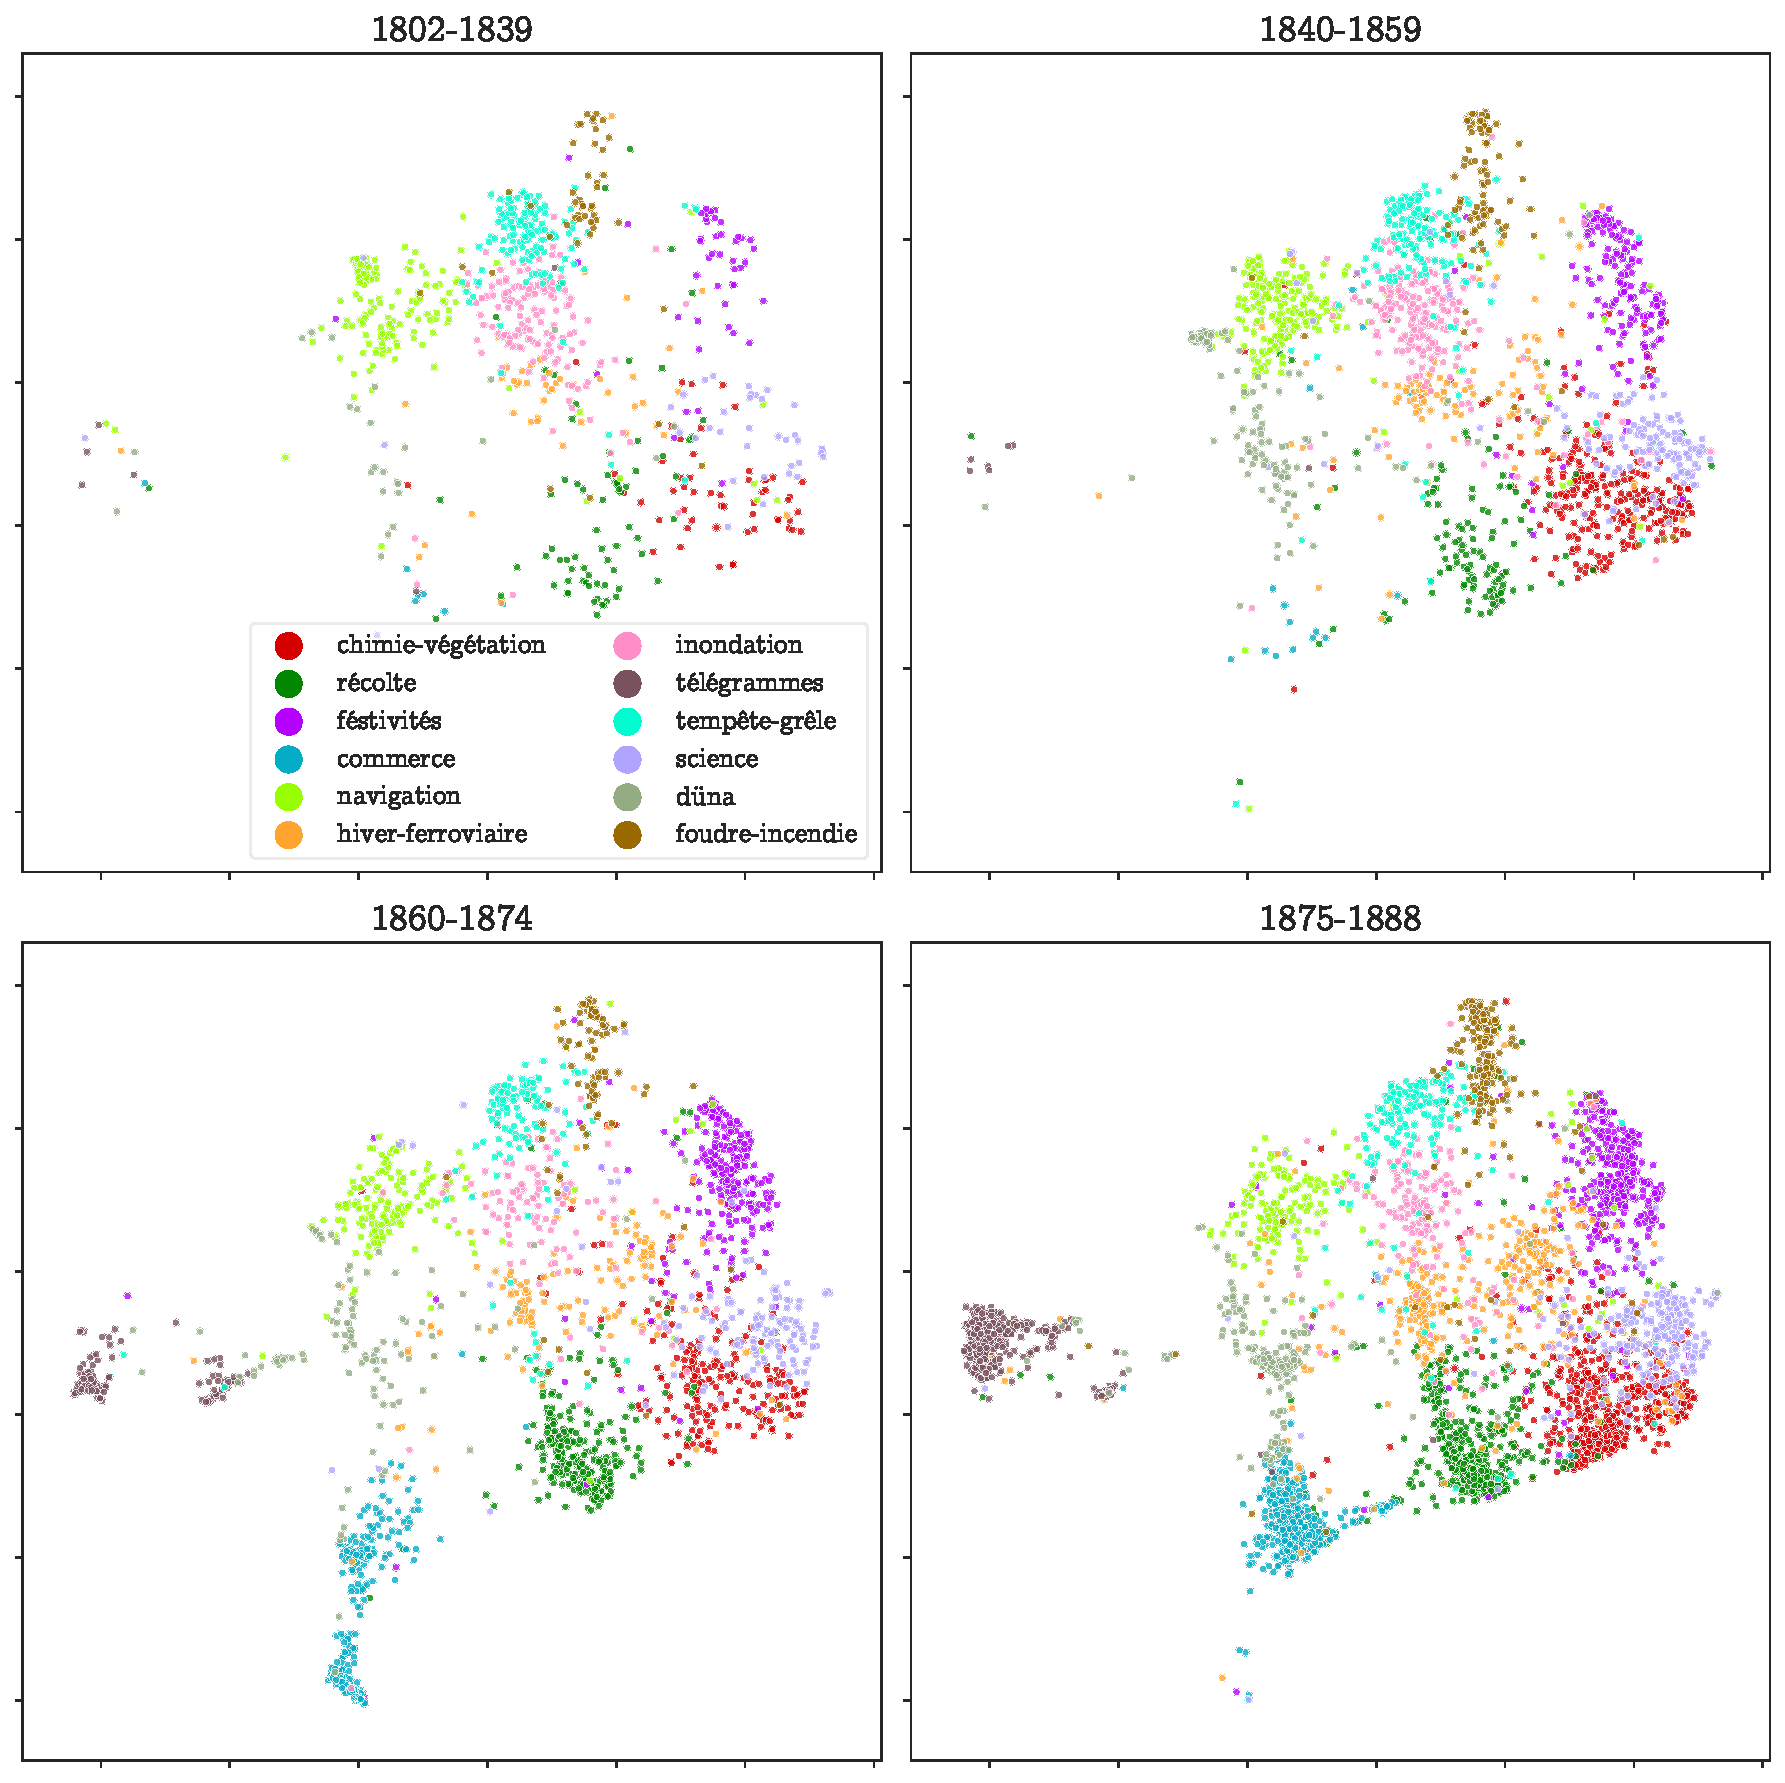
\includegraphics[width=\textwidth]{images/topics_umap_periods.pdf}
    \caption{Visualisation spatiale des sujets, divisée en quatre périodes}
    \label{fig:topics_umap_periods}
\end{figure}

Une autre possibilité d'analyse consiste à intégrer la dimension temporelle. La figure \ref{fig:topics_umap_periods} montre une projection UMAP de tous les segments, mais divise la plage temporelle en quatre périodes. Pour chaque fenêtre, seuls les segments qui ont été publiés pendant la période correspondante sont présentés. Les périodes ont été choisies pour refléter au mieux les changements thématiques, ainsi que pour compenser le déséquilibre temporel des données, la majorité des textes étant issus des dernières décennies de la période d'observation. Le positionnement des points sur ces graphiques peut légèrement différer de celui de la figure \ref{fig:topic_umap}, en raison de deux exécutions distinctes de l'algorithme UMAP.

La vue temporelle montre approximativement quand les différents sujets ont commencé à se former. Par exemple, on peut constater que les sujets \textit{tempête-grêle}, \textit{navigation} et \textit{inondation} sont les plus constants tout au long du siècle. On pourrait même dire que les nuages correspondants sont les plus cohérents pendant la période 1840-1859 et non dans les périodes ultérieures, malgré l'augmentation des données. Quatre autres thèmes, à savoir \textit{festivités}, \textit{science}, \textit{chimie-végétation} et \textit{récolte}, ont quelques occurrences entre 1802 et 1839, mais se forment beaucoup plus clairement dans la période 1840-1859. A partir de 1860, nous pouvons voir l'apparition soudaine de deux autres sujets, \textit{télégrammes} et \textit{commerce} - ceci correspond à l'analyse des sections précédentes. Le sujet \textit{düna}, par contre, est déjà visible entre 1840 et 1859. Enfin, la formation de \textit{hiver-ferroviaire} est à nouveau la plus floue, le nombre de points augmentant régulièrement à chaque période mais ne formant jamais un nuage aussi cohérent que les autres.

%\begin{figure}[h]
%    \centering
%    \includegraphics[width=0.7\textwidth]{im%ages/conceptual_scatterplot.pdf}
%    \caption{Comparaison conceptuelle des %sujets}
%    \label{fig:conceptual_scatterplot}
%\end{figure}

Ces niveaux d'analyse permettent de tenter de généraliser tous les thèmes liés au climat dans le \textit{Rigasche Zeitung}. Il me semble raisonnable de considérer que tous les thèmes sont placés sur deux axes théoriques, unique-répétitif et descriptif-numératif. La figure \ref{fig:conceptual_scatterplot} montre une manière possible de comparer les thèmes entre eux sur ces échelles conceptuelles. La taille des cercles correspond au nombre de segments pour chaque sujet, mais leur positionnement totalement intuitif et ne repose sur aucune donnée empirique. Néanmoins, je pense qu'elle résume les différences les plus fondamentales entre tous les sujets décrits et leur rôle dans la presse.

\begin{wrapfigure}{r}{0.6\textwidth}
  \begin{center}
    \includegraphics[width=0.6\textwidth, frame]{images/conceptual_scatterplot.pdf}
  \end{center}
  \vspace*{-2ex}
  \captionsetup{justification=centering}
  \caption{Comparaison conceptuelle des sujets}
  \label{fig:conceptual_scatterplot}
\end{wrapfigure}

Plus précisément, la figure aide à répondre à la question \og en quoi les informations sur le climat et sur le temps constituent-elles des nouvelles ? \fg{} En tenant compte de l'analyse de ce chapitre, on peut dire que dans les premières décennies du 19\textsuperscript{ème} siècle, les informations météorologiques ont principalement trouvé leur chemin vers la presse sous la forme d'événements spécifiques qui ont été rapportés. Une partie notable de ces informations concernait à son tour des événements extrêmes qui avaient souvent des effets socio-économiques négatifs. Dans ces textes, le climat pouvait être considéré comme le sujet des événements : toujours présent lors des célébrations et des rassemblements, même sans invitation ; capable de ruiner les récoltes et de couler les navires sur son caprice. Peu à peu, cependant, une autre vision du climat s'est imposée dans la presse, en le rendant un objet d'explication. C'est l'apparition de textes scientifiques, botaniques et agro-économiques qui pensent au climat de manière abstraite - non pas comme des événements uniques mais comme un élément sous-jacent du monde physique qu'il faut étudier et exposer. Enfin, dans la seconde partie du siècle et surtout à partir des années 1860, la presse commence à rendre compte du climat de manière systématique et répétitive. Le climat s'est ainsi intégré à d'autres informations comme les cours de la bourse, les horaires de train et les rapports de navigation. Ces trois modes de présentation de l'information ne se sont pas substitués les uns aux autres mais ont plutôt existé en parallèle.

[Ici encore un paragraphe pour finir le chapitre et avant de passer à la discussion etc?]



























\clearpage
\clearpage

\section{Analyse}

Avec les paramètres indiquées en haut, il est possible de décrire le jeu de données dans plusieurs manières.\footnote{Les données obtenues après le prétraitement se trouvent dans le fichier \texttt{./data/processed/LNB\_processed.xlsx}. Les analyses sont disponibles dans le \textit{notebook} \href{https://github.com/krkryger/clim-dist/blob/main/notebooks/01-first-data-exploration.ipynb}{\texttt{01-first-data-exploration.ipynb}}} Dans un premier temps, la distribution temporelle des données semble de correspondre assez logiquement à l'augmentation constante de la volume de la presse pendant le 19\textsuperscript{e} siècle (figure \ref{fig:data_hist}). Evidemment, cette croissance ne reflète pas un développement spécifique du climat dans la région baltique. En effet, séparer les changements climatiques potentiels de la variation dans la quantité des données disponibles sera l'un des défis les plus importants de cette recherche.

%\begin{figure}[h]
%\centering
%\includegraphics[width=\textwidth]{images/distribution_temp_journaux.png}
%\caption{La distribution temporelle des données}
%\label{fig:data_hist}
%\end{figure}

Le jeu de données contient 46 journaux uniques. Leur distribution est inégale : le journal le plus représenté, \textit{Rigasche Zeitung} (le journal de Riga) compte pour un tiers de tous les articles. Les deux journaux les plus répandue composent une moitié du \textit{dataset}, les 5 plus nombreux presque 80\%. La distribution des toutes les revues est présenté dans la figure \ref{fig:publications}, accompagné des noms des revues les plus populaires.

\begin{figure}[!h]
\centering
\includegraphics[width=\textwidth]{images/distribution_proportionnelle_journaux.png}
\caption{La distribution temporelle des articles selon les journaux}
\label{fig:publications}
\end{figure}

\begin{figure}[!h]
\begin{minipage}{0.5\textwidth}
    \centering
    \includegraphics[width=0.9\linewidth]{images/w_count.png}
    \captionsetup{width=.8\linewidth}
    \caption{Longueur des articles en mots séparés par des espaces}
    \label{fig:w_count}
\end{minipage}
\begin{minipage}{0.5\textwidth}
    \centering
    \includegraphics[width=0.9\linewidth]{images/text_len.png}
    \captionsetup{width=.8\linewidth}
    \caption{Longueur des articles en caractères}
    \label{fig:text_len}
\end{minipage}
\end{figure}

Les figures \ref{fig:w_count} et \ref{fig:text_len} démontrent la longueur des textes dans le corpus. Comme indiqué plus haut, le nombre des \og mots \fg{} a été simplement calculé en divisant les textes par des espaces. Cette valeur est donc indicative est ne correspond pas exactement au nombre des mots dans un texte quelconque, à cause des erreurs de transcription, segmentation etc. Les longueurs des textes nous montrent deux choses importantes. Premièrement, la fréquence des textes diminue avec la croissance de leur longueur. Deuxièmement, il existe un pic irrégulier au milieu des textes les plus longs qui est le plus visible dans la figure \ref{fig:text_len}. Une vue de plus près nous renseigne qu'il existe 1918 entrées qui comptent 32767 caractères, la valeur maximale présente dans le jeu de données. En regardant les articles en question sur periodika.lv, il parait que la segmentation des articles a été défectueuse et que les différents articles et sections d'un numéro ont été empilé jusqu'à ce que la longueur apparente du fichier à été atteinte. Par extension, ces textes contiennent bien de l'information potentiellement importante, mais il peuvent présenter des défis complexes par rapport à la division des parts pertinents et non pertinents.

Le fait que tous les textes sont accompagnés par un titre de l'article nous permet d'avoir un aperçu général des sujets les plus répandus. Il convient de noter que la structuration de l'information textuelle, dont les origines étaient déjà présentes au 17e siècle, assez constante pendant la période observée. L'élément le plus caratéristique de cette structure est la division des nouvelles par les points d'origine - ainsi, un \og sous-chapitre \fg{} d'un numéro commence normalement avec le nom d'une ville d'où l'information a été reçue, et parfois la date. Cette particule du texte fait le plus souvent partie d'un chapitre majeur du numéro - nouvelles étrangères, la commerce etc. Cela nous ramène au problème de la segmentation - parfois, il n'est pas complètement clair si un article quelconque doit être considéré comme une section et sous-section, même en observant le journal original. En conséquence, le champ \texttt{head} peut bien contenir l'un des deux, selon la décision de segmentation qui a été faite. Les noms d'articles les plus courants dans la totalité des données avec leurs nombres et les traductions françaises approximatives sont représenté dans le tableau \ref{tab:article_titles}.

\begin{table}[h]
    \centering
    \footnotesize
    \begin{tabular}{|l|r|}
    \hline
         Inland (\textit{actualités nationales}) & 3131 \\
         Ausland (\textit{actualités étrangères}) & 2862 \\
         Locales/Lokales & 1898 \\
         Vermischtes (\textit{varia}) & 1031 \\
         Frankreich (\textit{la France}) & 562 \\
         Feuilleton & 445 \\
         Telegramme & 387 \\
         St. Petersburg & 379 \\
         Deutschland (\textit{l'Allemagne}) & 376 \\
         Handel und Verkehr (\textit{commerce et transport}) & 370 \\
         Neueste Nachrichten (\textit{dernières nouvelles}) & 364 \\
         Vermischte Nachrichten (\textit{nouvelles mélangées}) & 338 \\
         Rigasche Zeitung & 313 \\
         Bekanntmachungen (\textit{annonces}) & 295 \\
         Inländische Nachrichten (\textit{actualités nationales}) & 290 \\
         Riga & 254 \\
         Oesterreich (\textit{l'Autriche}) & 249 \\
         Italien (\textit{l'Italie}) & 219 \\
         Orientalische Angelegenheiten (\textit{affaires orientales}) & 199 \\
         England (\textit{l'Angleterre}) & 180 \\
    \hline
    \end{tabular}
    \caption{Les 20 titres d'articles les plus fréquents}
    \label{tab:article_titles}
\end{table}

\clearpage

Le changement quantitatif autour des années 1840 visible sur les graphiques précédents se révèle d'être qualitatif aussi. L'on peut observer qu'à partir du milieu du siècle, les journaux se focalisent plus sur les nouvelles nationales et locales. Cela signalise une rupture importante par rapport au rôle du journalisme : auparavant, les journaux s'occupaient principalement des affaires lointaines, tandis que les informations locales étaient moins différenciées et se trouvaient habituellement dans des catégories mélangées. Ce changement de l'accent vers l'intérieur (qui devrait être mieux décrit et quantifié) et mon expérience antérieure avec les sources permettent de formuler une hypothèse que le public devenait plus attentif au climat autour de lui pendant le 19\textsuperscript{e} siècle, ou peut-être que le climat a obtenu un caractère plus précis et énoncé dans la vie des gens. Les changements proportionnels des titres d'articles sont visibles sur la figure \ref{fig:titles_lineplots}, séparé en deux pour prendre en compte la différence mentionnée (à noter les échelles différentes). 

\begin{figure}[h]
\begin{subfigure}
    \centering
    \includegraphics[width=\textwidth]{images/titres_1800_1850.png}
\end{subfigure}
\begin{subfigure}
    \centering
    \includegraphics[width=\textwidth]{images/titres_1850_1900.png}
\end{subfigure}
\caption{Les titres les plus prévalents en 1800-1850 et 1850-1900}
\label{fig:titles_lineplots}
\end{figure}

Comme expliqué plus haut, les données ont été obtenues par recherche textuelle des trois mots clés. Il convient maintenant de noter que la prévalence de ces mots varie considérablement. Notamment, environ 88\% des entrées contiennent le mot \textit{Sturm}, tandis que les taux ne sont que 12\% et 9\% pour \textit{Hagel} et \textit{Überschwemmung}, respectivement. Cela nous amène à la question de \textbf{l'ambiguïté}. A la différence de \textit{Hagel} et \textit{Überschwemmung}, les emplois de \textit{Sturm} sont beaucoup plus variés et peuvent avoir des contextes complètement sans rapport au temps. Premièrement, \textit{Sturm} est un nom de famille assez répandu en allemand. Deuxièmement, il a souvent un sens métaphorique (une tempête (fureur) politique, une tempête des sentiments, etc.) et fait partie des plusieurs expressions idiomatiques (\textit{im Sturm nehmen} - prendre l'assaut, \textit{die Stille vor dem Sturm} - le calme avant la tempête, \textit{der Sturm im Wasserglas} - la tempête dans un verre d'eau, etc. etc.). Troisièmement, \textit{Sturm} est un élément très courant dans la poésie romantique allemande souvent publié dans les journaux (comme d'autres ). L'effet sur les données est évident : p. ex., il est très probable que le pic vers le milieu des années 1850 visible sur les figures \ref{fig:data_hist} et \ref{fig:publications} soit lié à la guerre de Crimée, très largement réfléchie dans le médias.

A partir des telles observations, l'on peut définir au moins quatre facteurs qui influencent la fréquence d'un mot \og climatique \fg{} dans les données :
\vspace{1ex}
\begin{itemize}[label=$\bullet$]
    \item La vraie fréquence du phénomène météorologique lui-même
    \item Son impact sur la société humaine qui le rend plus intéressant pour les médias
    \item L'existence des emplois parallèles, c.-à-d. des idiomes, métaphores et noms communs
    \item La volume absolue des médias
\end{itemize}
\vspace{2ex}

On commence a voir la complexité qui émerge par rapport aux futurs buts de recherche. Comment serait-il possible de séparer tous ces facteurs pour arriver à une hypothèse sur la fréquence et le caractère des phénomènes météorologiques tels qu'ils ont réellement eu lieu ? La perspective de schématiser les tendances vraies du climat au cours du 19\textsuperscript{e} siècle parait assez difficile en ce moment. En revanche, une analyse et comparaison de ces facteurs permettrait de donner la réponse aux autres questions : comment le regarde \og climatique \fg{} de la société a-t-il tourné vers l'intérieur du pays et s'accentué ? Une possibilité de le faire serait d'écarter l'approche par les mots clés et se concentrer sur un corpus mieux délimité pour avoir une meilleure représentation de la masse du journalisme pendant la période observé. J'ai déjà reçu un deuxième jeu de données de LNB qui contient tous les numéros de \textit{Rigasche Zeitung}, le journal qui compte pour un tiers du corpus actuel et qui a paru régulièrement tout au long du 19\textsuperscript{e} siècle. Ceci étant dit, le choix des mots clés nous permet d'avoir une concentration plus élevée des mentions météorologiques et des faux-positifs, une circonstance qui facilite l'entraînement du modèle NER que nous verrons dans le chapitre suivant.

\clearpage












\section{Détection des phénomènes météorologiques}

Dans un sens plus général, la tâche de la détection des différents phénomènes météorologiques appartient au domaine d'extraction d'événements. Ce domaine de recherche a retenu une attention considérable dans les dernières décennies, mais surtout par rapport aux sujets comme la biomédecine\footcite[P. ex.][]{wang_multiple_2017}, réseaux sociaux\footcite{sefh_detection_2020} etc., mais parmi les approches utilisées, allant des simples techniques comme TF-IDF aux réseaux de neurones complexes, seulement quelques-unes ont été appliquées à l'histoire.\footcite{sprugnoli_novel_2019} Même dans les manuels plus avancés comme celui de Jurafsky et Martin, le sujet de l'extraction d'événements n'est abordé que très sommairement et avec des exemples venant des données bien adaptées pour cette tâche en particulier.\footcite[348-350]{jurafsky_speech_2020} La situation avec les données historiques et malheureusement beaucoup plus compliquée : les différentes sources de bruît, les variations historiques de la langue, un changement relatif des modalités de description, des noms des lieux etc. sont tous des éléments qui démontrent la spécificité des approches nécessaires. Cependant, presque tous les travaux qui concernent un sujet comparable au nôtre semblent d'employer un composant de la \textbf{reconnaissance d'entités nommées} (NER - \textit{Named Entity Recognition}) et une ontologie d'événements approprié au domaine en question.

L'un des traitements sur le sujet de l'extraction d'événements les plus récents et les plus détaillés avec un accent sur les données historiques et celui de Rachele Sprugnoli et Sara Tonelli.\footcite{sprugnoli_novel_2019} Dans leur article, elles proposent les directives pour une annotation d'événements (basées sur l'anglais) et appliquent un classificateur CRF (\textit{Conditional Random Field}) et un réseau BiLSTM (\textit{Bidirectional Long Short-Term Memory}) pour les détecter dans un corpus de récits de voyage et de journaux. Après avoir testé des différentes configurations pour les deux modèles, elles ont réussi d'atteindre une \textit{F-score} de 83,62\% pour la tâche de la détection et 64,39\% pour la détection \textit{et} la classification des événements dans les 22 catégories d'événements définies. Le modèle BiLSTM a rendu les meilleurs résultats dans les deux cas.\footcite[][257]{sprugnoli_novel_2019}

A partir de cette étude et d'autres, j'ai décidé d'entraîner un modèle de NER avec la bibliothèque SpaCy de Python pour aborde le problème de détection. Après des premières investigations, il s'est avéré que le module allemand de base de SpaCy (\texttt{de\_core\_news\_md}) est en fait assez bien capable de traiter le corpus historique du projet. P. ex., en appliquant le \textit{pipe} NER à l'exemple présenté au début du chapitre précendent dans le tableau \ref{table:ocr}, l'on obtient les catégories des entités dans le tableau \ref{tab:first_ner_example}.

\begin{table}[!h]
    \centering
    \begin{tabular}{|l|l|l|l|}
    \hline
        Riga\textbackslash nPisa & \texttt{ORG} & Jtn Freien\textbackslash n & \texttt{MISC}  \\
        Wirst-z & \texttt{PER} & Drolligistes & \texttt{LOC} \\
        Jttdeß & \texttt{LOC} & Meirz & \texttt{LOC} \\
        \textbf{Ileberschetnntuttgen}\textbackslash n & \texttt{ORG} & \textbf{Sturm} & \texttt{MISC} \\
        Vollwerks & \texttt{LOC} & \textbf{Hagel} & \texttt{PER} \\
        Thermosneter & \texttt{LOC} & \textbf{Sturm} & \texttt{MISC} \\
    \hline
    \end{tabular}
    \caption{Exemple de la performance initiale du modèle NER de SpaCy}
    \label{tab:first_ner_example}
\end{table}

Evidémment, SpaCy ne sait pas reconnaître les phénomènes météorologiques parce qu'une telle catégorie d'entités n'est pas présente dans sa configuration de base. En revanche, il a attribué des étiquettes des autres catégories (\texttt{PER}, \texttt{MISC}, \texttt{ORG}) aux mots avec une signifiance météorologique (marqués en gras dans le tableau \ref{tab:first_ner_example}).

Avant de procéder à l'entraînement du modèle NER, la question doit être posée : \og qu'est-ce que c'est qu'un événement climatique ? \fg{}. Bien sûr, il s'agit d'un changement d'état de l'atmosphère qui est observable et mesurable par des variables comme la température, la pression de l'air, la précipitation etc - mais ces variables sont rarement traduites directement aux narratives qui se trouvent dans les sources historiques. L'un des problèmes les plus importants qui surgissent est celui de l'étendue temporelle et spatiale. Un \og événement \fg{} peut être plus ou moins discret. Prenons par exemple la tempête - un phénomène dont le début et la fin sont assez bien délimités dans la perspective du bon sens, l'instrument habituel de chacun qui n'est pas météorologue. Une tempête est bien plus discrète dans le temps et dans l'espace qu'une sécheresse dont les limites sont contestables - est-ce qu'elle débute avec les premiers jours chauds ou seulement quand son effet sur la récolte commence à se manifester ? Aujourd'hui, il est possible de répondre à ces questions assez nettement avec les réseaux modernes de stations d'observation et à l'aide du progrès de la science météorologique, mais les réponses obtenues n'ont pas beaucoup à voir avec la perception moyenne des personnes du 19\textsuperscript{e} siècle. Il faut prendre en compte qu'en ce temps-là, les descriptions du temps présentes dans les sources reflètent l'expérience direct de l'auteur ou l'un de ses informateurs, en tout cas se délimitant au monde immédiatement observable.

C'est en gardant ces considérations à l'esprit que nous approchons de la reconnaissance des entités nommées. Pour arriver d'abord à un modèle si simple et robuste que possible, j'ai décidé de laisser à côté de la durée temporelle des événements et me concentrer seulement sur la détection \og absolue \fg{} d'eux. Par conséquence, les catégories avec lesquelles l'annotation des données a été réalisée étaient les suivantes :
\vspace{1ex}
\begin{itemize}[label=$\bullet$]
    \item \texttt{LOC} : toutes sortes de noms de lieux;
    \item \texttt{DAT} : les dates;
    \item \texttt{WEA} : les mots signifiant des phénomènes climatiques;
    \item \texttt{MEA} : les mesures/les observations instrumentales;
    \item \texttt{PER} : les noms de personnes
\end{itemize}
\vspace{2ex}

Les autres catégories déjà présentes dans SpaCy (\texttt{MISC}, \texttt{ORG}) étaient parfois employées pour l'annotation, p. ex de designer les noms de navires (souvent liés aux événements maritimes) et les noms de revues (par rapport à la circulation de l'information), mais elles ne sont pas centrales à l'analyse et ne sont pas évaluées. Il s'en va de même pour \texttt{MEA} qui était plutôt une catégorie experimentale mais qui n'a pas rendu des résultats utilisables. Les catégories clés pour détecter les événements sont donc les trois premières : \texttt{LOC}, \texttt{DAT} et \texttt{WEA}. En se basant sur l'approche de Seffih \textit{et al.}\footcite[175]{sefh_detection_2020}, nous pouvons formuler un événement comme suit : $E = (P,L,D)$ où $P = f_{phenomene}({source}_n)$, $L = f_{lieu}({source}_n)$ et $D = f_{date}({source}_n)$. La catégorie \texttt{PER} sert d'un outil de désambiguïsation - les noms de personnes ne sont pas importantes dans la détection d'événements climatiques, mais elles sont souvent retrouvées comme entités par SpaCy. Une bonne détection de noms de personnes est donc nécessaire pour éviter des faux-positifs dans les autres catégories.

L'entraînement du modèle NER a été réalisé en deux étapes conséquentes. Les règles de l'annotation, le processus de l'entraînement et les évaluations sont décrits dans le reste de ce chapitre.

\subsection{Directives d'annotation}

La tâche de l'annotation présente des nombreuses difficultés et de cas limites dans le sens sémantique ainsi qu'ortographique. Cela vaut en particulier pour les catégories non standards : \texttt{WEA} et \texttt{DAT}. Pour la catégorie \texttt{WEA}, les difficultés suivantes s'ont produites :
\vspace{1ex}
\begin{itemize}[label=$\bullet$]
    \item \textbf{Le caractère linguistique d'un phénomène}. Il peut s'exprimer comme un simple substantif (\textit{Wind} - le vent), un mot composé (\textit{Nordwestwind} - vent de nord-ouest), un verbe composé (\textit{gestern hat \textbf{es} den ganzen Tag \textbf{geregnet}} - hier, il a plu toute la journée) ou même un adjectif (\textit{die letzte Woche ist sehr \textbf{windig} gewesen} - la semaine dernière a été très venteuse).
    \item \textbf{Les séparations problématiques de mots}. Comme indiqué dans le Chapitre 1, les fins des lignes sont souvent été exclues du texte océrisé. Dans le cas d'un mot composé, le tiret qui signifierait l'unité des deux parts peut donc être absent. Si l'on choisit de les étiqueter comme une seule entité, on obtient le symbole de saut de ligne (\texttt{\textbackslash n}) au milieu de l'entité, qui peut causer un décalage de \textit{tokenisation} de SpaCy à son tour.
    \item \textbf{Les erreurs d'OCR}. Au cours de l'océrisation, des symboles peuvent avoir été omis du texte et d'autres peuvent avoir été ajoutés.
\end{itemize}
\vspace{2ex}

A partir des problèmes ci-dessus, les directives générales d'annotation qui suivent ont été formées :
\vspace{1ex}
\begin{enumerate}
    \item Considérer toutes les sortes d'expressions linguistiques mentionnées comme d'entités;
    \item Considérer les mots composés, ainsi que les mots qui \textit{devraient} être composés dans le sens grammatical, mais ne le sont pas (c'est-à-dire qu'ils sont séparés par des espaces à cause d'OCR ou d'incohérence grammaticale dans la source elle-même) comme une seule entité;
    \item Pour les verbes, inclure également les verbes auxiliaires si et seulement s'ils sont adjacents l'un à l'autre dans la phrase;
    \item Considérer les mots coupés par un saut de ligne comme une seule entité;
    \item Dans le cas des erreurs d'OCR, considérer le mot comme une entité si sa forme grammatical est intelligible pour l'annotateur (dans la pratique, le taux d'erreur acceptable dans un mot est environ 50\% au niveau des caractères);
    \item Pour les entités \texttt{DAT}, inclure l'étendue maximale de l'information, y compris les abréviations courantes comme \textit{d. M.} ou \textit{c.} (signifiant le mois en cours);
    \item Pour les entités \texttt{PER}, inclure les noms et tous les prénoms, mais pas de poste; inclure les titres de noblesse si et seulement s'ils sont accompagné par seul nom (p. ex \textit{\textbf{Graf Menningshof}}, mais \textit{Graf \textbf{Ludwig von Menningshof}}).
\end{enumerate}
\vspace{2ex}

Il est vrai que la décision d'inclure même des verbes et adjectifs peut introduire des difficultés pour SpaCy, mais trop d'information est exprimé sous ces formes pour les écarter. Sprugnoli et Tonelli ont également utilisé des directives qui englobaient des très diverses formes grammaticales.\footcite[233-236]{sprugnoli_novel_2019}. Toutefois, les règles définis ici sont sujets à l'amélioration future pour mieux prendre en compte la particularité des questions de recherche et des sources. Elles sont donc à considérer comme une première ébauche et leur application correcte et unifiée aux données d'annotation devrait également être vérifié avant les prochaines étapes du travail en M2.


\subsection{Première annotation}

Le premier lot d'annotation a été commencé avant que LNB avait fourni le corpus.\footnote{Le \textit{notebook} correspondant à ce sous-chapitre est \href{https://github.com/krkryger/clim-dist/blob/main/notebooks/03-storms-annotation-test.ipynb}{\texttt{03-storms-annotation-test.ipynb}}} Pour utiliser directement des données externes, sans avoir à attendre le corpus et le diviser en un ensemble de formation et un ensemble de test, les données collectées auparavant dans le carde du projet de recherche de l'Université de Tallinn ont été employées.\footnote{\texttt{./data/processed/storms\_for\_annotation.xlsx}} Ce corpus du premier entraînement a, en partie, la même source d'origine que le corpus de LNB et est presque un sous-ensemble du dernier. Cependant, la différence de taille des deux corpora est très grande - le corpus d'entraînement consiste à 567 extraits avec une longueur moyenne de 242 caractères, tandis que le jeu de données de LNB compte plus de 33 000 entrées. Les textes venant du projet de l'Université de Tallinn avaient été recopiés à la main depuis les journaux numérisés et considérablement nettoyés (fautes d'OCR, sauts de ligne etc.). Cela explique aussi la longueur beaucoup plus faible que la moyenne des textes de LNB - seulement les parts comportant des informations pertinents sur l'événement climatique ont été gardées, parfois avec du texte omis de la source originelle. Cette choix a été fait pour ne pas perdre le temps en attendant le corpus de LNB et en espérant que le chevauchement partiel des deux \textit{datasets} n'empêchera trop l'évaluation.

Pour l'annotation, les textes analysés avec le modèle de base de SpaCy ont été importés au Doccano\footnote{\url{https://doccano.herokuapp.com/}} pour corriger et rajouter des étiquettes.\footnote{L'usage de Doccano a nécessité un \textit{script} sur mesure pour convertir les données entre les formats de Doccano et Spacy : \href{https://github.com/krkryger/clim-dist/blob/main/climdist/ner/doccano_transformations.py}{\texttt{doccano\_transformations.py}}. Les annotations réalisées se trouvent dans \href{https://github.com/krkryger/clim-dist/blob/main/pipeline/03_ner/01_doccano/storms_annotated_19.03v2.jsonl}{\texttt{./pipeline/03\_ner/01\_doccano/storms\_annotated\_19.03v2.jsonl}}}

\begin{figure}[h]
    \centering
    \includegraphics[width=\textwidth]{images/doccano1.png}
    \caption{Aperçu des données annotées dans Doccano}
    \label{fig:doccano1}
\end{figure}

Le modèle NER de SpaCy a été entraîné avec les paramètres suivants : 20 itérations, \texttt{size=compounding(4.0, 32.0, 1.001)}.\footnote{\texttt{./data/models/ECH\_storms\_ner\_model/}} Pour évaluer sa performance, un \textit{script} sur mesure a été créé. Le problème principal de l’évaluation venait des erreurs de la segmentation, causés par l’OCR. Les limites d’une entité ne correspondaient pas toujours nettement à la tokenisation de Spacy, un fait qui a pose une difficulté pour la mesure de la précision et du rappel au niveau du \textit{token}. Par exemple, quelques-uns de ces différences étaient causés par le fait que Spacy compte les sybmoles ‘«’ et ‘»’ comme des \textit{tokens} – en conséquence, les entités peuvent parfois commencer et finir au milieu d’un seul token.
Pour cette raison, une méthode d’évaluation assez lâche a été choisie. A ce point, la question des limites exactes des entités n’est pas d’une haute importance comparées à leur présence ou absence. En conséquence, \textit{la catégorisation d'un \textit{token} a été considérée correcte s'il y avait au moins un chevauchement d'une entité de la même étiquette dans l'ensemble de validation}.

Pour présenter l'approche d'évaluation d'une manière la plus claire possible, il convient d'inclure la totalité du \textit{script}\footnote{\href{https://github.com/krkryger/clim-dist/blob/main/climdist/ner/evaluation.py}{\texttt{./climdist/ner/evaluation.py}}} :

\begin{minted}[fontsize=\scriptsize, bgcolor=lightgray, baselinestretch=0.8, frame=lines, linenos]{python}
def evaluate_ner(pred, gold):
    
    '''Inputs are a Spacy NLP object and a gold standard annotation.
    Returns two a tuple of two lists of booleans, first for gold standards, second for predictions.
    Lists can later be compared with Scikit-learn.confusion_matrix to get TP, FP, TN, FN scores.'''
    
    types_labels = {0:0}
    for ent in pred.ents:
        types_labels[ent.label] = ent.label_
        
    pred_tokens = []
    pred_entities = []
    pred_positions = []
    
    for token in pred:
        pred_tokens.append(token)
        pred_entities.append(types_labels[token.ent_type])
        pred_positions.append((token.idx,token.idx + len(token)))
        
    gold_tokens = []  
    for pos in pred_positions:
        gold_tokens.append(gold['text'][pos[0]:pos[1]])
    
    entity_set = []
    for ent in gold['entities']:
        if ent[2] not in entity_set:
            entity_set.append(ent[2])
     
    gold_entity_ranges = {}
    
    for ent in entity_set:
        entpos = []
        for entity in gold['entities']:
            if entity[2] == ent:
                entpos += (list(range(entity[0], entity[1])))
        gold_entity_ranges[ent] = entpos
            
    gold_entities = []
    
    for pos in pred_positions:
        isentity = False
        for label in entity_set:
            if set(range(pos[0], pos[1])) & set(gold_entity_ranges[label]):
                isentity = True
                gold_entities.append(label)
                break
        if not isentity:
            gold_entities.append(0)
    
    results = {}
    
    for label in entity_set:
        label_gold = [1 if ent==label else 0 for ent in gold_entities]
        label_pred = [1 if ent==label else 0 for ent in pred_entities]
        
        results[label] = (label_gold, label_pred)
        
    return results




def evaluation_results(predictions, gold_data, allowed_labels, output_dir=None, cmap='viridis'): 
    
    from sklearn.metrics import confusion_matrix
    from sklearn.metrics import ConfusionMatrixDisplay
    
    total_gold = []
    total_pred = []
    
    for prediction, annotation in zip(predictions, gold_data):
        
        eval_scores = evaluate_ner(prediction, annotation)
        
        for label in list(eval_scores.keys()):
            if label in allowed_labels:
                total_gold += eval_scores[label][0]
                total_pred += eval_scores[label][1]
            
    matrix = confusion_matrix(total_gold, total_pred)
    print(matrix)
    
    tn, fp, fn, tp = matrix.ravel()

    print(allowed_labels)
    
    precision = tp/(tp+fp)
    recall = tp/(tp+fn)
    f_score = 2 / ((recall**-1) + (precision)**-1)
    
    print(f'precision: {precision}, recall: {recall}, f-score: {f_score}')
    print('\n')
    
    cmplot = ConfusionMatrixDisplay(matrix)
    cmplot.plot()
    cmplot.ax_.set(title='  '.join([label for label in allowed_labels]))
    cmplot.im_.set_cmap(cmap)
    
    if output_dir:
        plotname = '_'.join([label for label in allowed_labels])
        cmplot.figure_.savefig(output_dir + 'cm_' + plotname + '.png', bbox_inches='tight')
\end{minted}

Pour l'évaluation, nouveaux textes d'une longueur de moins de 150 mots (selon l'attribut \texttt{w\_count}) ont été choisis aléatoirement et annotés à la main, afin de créer un ensemble \textit{gold}. Avec le code ci-dessus, l'on obtient les résultats suivants pour le premier modèle NER\footnote{Le \textit{notebook} qui présente les résultats de l'évaluation est \href{https://github.com/krkryger/clim-dist/blob/main/notebooks/ner-custom-eval.ipynb}{\texttt{./notebooks/ner-custom-eval.ipynb}}} :

\begin{figure}[h]
\centering
\begin{subfigure}
    \centering
    \includegraphics[width=0.3\textwidth]{images/cf_mat1/cm_LOC.png}
\end{subfigure}
\begin{subfigure}
    \centering
    \includegraphics[width=0.3\textwidth]{images/cf_mat1/cm_WEA.png}
\end{subfigure}

\begin{subfigure}
    \centering
    \includegraphics[width=0.3\textwidth]{images/cf_mat1/cm_DAT.png}
\end{subfigure}
\begin{subfigure}
    \centering
    \includegraphics[width=0.3\textwidth]{images/cf_mat1/cm_PER.png}
\end{subfigure}
\caption{Matrices de confusion pour le premier modèle NER}
\label{fig:conf_mat1}
\end{figure}

Les résultats généraux pour toutes les quatre catégories des entités sont les suivants :
\vspace{1ex}
\begin{itemize}[label=$\bullet$]
    \item \texttt{Précision : 0,70}
    \item \texttt{Rappel : 0,51}
    \item \texttt{F-score : 0,59}
\end{itemize}
\vspace{2ex}

\clearpage

Comme le montrent les matrices de confusion en haut, le modèle a été le plus efficace performant dans la catégorie \texttt{DAT} ($P=0,9, R=0,69, F=0,78$) - sans doute en raison de l'incorporation des caractères numériques et d'un format assez constant qui rendent l'information des dates assez bien distinguable des autres catégories. Les scores ont été $P=0,58, R=0,64, F=0,61$ pour \texttt{WEA} et $P=0,62, R=0,52, F=0,57$ pour \texttt{LOC}. La catégorie avec les résultats les plus faibles a été \texttt{PER} ($P=0,69 R=0,34 F=0,45$), à cause de manque presque total des noms de personnes dans l'ensemble d'entraînement.





\subsection{Deuxième annotation}

Le deuxième tour de l'entraînement a été réalisé avec des données issues du corpus de LNB. 200 textes d'une longueur maximale de 150 mots ont été choisis d'une façon automatique, mais quand-même filtrés à la main pour éviter des textes dont la qualité d'OCR est tellement faible qu'elle ait un effet négatif sur l'entraînement. Ces textes étaient beaucoup plus variés que ceux de la première annotation, car ils contenaient aussi des textes faux-positifs, c’est-à-dire ceux dans lesquels il ne s’agissait pas d’un vrai phénomène météorologique.

\begin{figure}[!h]
\begin{subfigure}
\centering
    \includegraphics[scale=0.4]{images/doccano3.png}
\end{subfigure}
\begin{subfigure}
\centering
    \includegraphics[scale=0.4]{images/doccano4.png}
\end{subfigure}
\caption{Exemples de la deuxième annotation - une liste de personnes et une table de matières du journal}
\label{fig:doccano3_4}
\end{figure}

La variance augmentée dans les sources a été nécessaire pour permettre à SpaCy de reconnaître des entités nommées dans des différents genres du texte. Dans l’échantillon, il se trouvait par exemple des notices nécrologiques, des rapports de guerre, des poèmes etc., etc. L'échantillon comportait également une plus grande variance de noms de lieux, parce que tous les textes de la première annotation avaient décrit la région baltique.\footnote{Les annotations se trouvent dans \href{https://github.com/krkryger/clim-dist/blob/main/pipeline/03_ner/01_doccano/annotated_data_250421.jsonl}{\texttt{./pipeline/03\_ner/01\_doccano/annotated\_data\_250421.jsonl}}}

En général, le processus de l'annotation demandait beaucoup plus d'attention cette fois - des nouvelles décisions ont été prises sur-le-champ pour arriver à une connaissance plus complète des règles optimales de l'annotation. Il est important de noter encore une fois qu'il reste encore quelques incohérences dans les annotations à cause de l'apparition des nouveaux cas sémantiques qui pouvaient modifier les détails des directives. Cependant, même avec la certaine irrégularité dans l'ensemble \textit{gold}, les résultats de NER s'ont considérablement amélioré après un nouveau entraînement avec les mêmes paramètres que la première fois\footnote{Le modèle se trouve dans \texttt{./data/models/spacy\_model\_250421/}, l'évaluation est visible dans le \textit{notebook} \href{https://github.com/krkryger/clim-dist/blob/main/notebooks/ner-custom-eval.ipynb}{\texttt{./notebooks/ner-custom-eval.ipynb}}} :

\begin{figure}[h]
\centering
\begin{subfigure}
    \centering
    \includegraphics[width=0.3\textwidth]{images/cf_mat2/cm_LOC.png}
\end{subfigure}
\begin{subfigure}
    \centering
    \includegraphics[width=0.3\textwidth]{images/cf_mat2/cm_WEA.png}
\end{subfigure}

\begin{subfigure}
    \centering
    \includegraphics[width=0.3\textwidth]{images/cf_mat2/cm_DAT.png}
\end{subfigure}
\begin{subfigure}
    \centering
    \includegraphics[width=0.3\textwidth]{images/cf_mat2/cm_PER.png}
\end{subfigure}
\caption{Matrices de confusion pour le deuxième modèle NER}
\label{fig:conf_mat2}
\end{figure}

La performance obtenue à travers de toutes les catégories se caractérise par les chiffres suivants :
\vspace{1ex}
\begin{itemize}[label=$\bullet$]
    \item \texttt{Précision : 0,84}
    \item \texttt{Rappel : 0,76}
    \item \texttt{F-score : 0,80}
\end{itemize}
\vspace{2ex}

\clearpage

Les résultats pour la catégorie \texttt{DAT} ont à nouveau été les meilleurs : $P=0,93, R=0,86, F=0,9$. La catégorie \texttt{LOC} a connu l'amélioration la plus significative avec les chiffres $P=0,89, R=0,78, F=0,83$. La catégorie \texttt{WEA} s'a amélioré à $P=0,83, R=0,73, F=0,78$, tandis que les scores pour \texttt{PER} ont été $P=0,73, R=0,68, F=0,7$

\begin{table}[h]
    \centering
    \begin{tabular}{l|l|l|}
         & 1\textsuperscript{e} modèle & 2\textsuperscript{e} modèle\\
         \hline
         LOC & 0,57 & 0,83\\
         WEA & 0,61 & 0,73\\
         DAT & 0,78 & 0,90\\
         PER & 0,45 & 0,70\\
         \textbf{Total} & \textbf{0,59} & \textbf{0,80}
    \end{tabular}
    \caption{Comparaison des \textit{F-scores} des deux modèles}
    \label{tab:f_scores}
\end{table}

Le tableau \ref{tab:f_scores} rend visible que les catégories dont l'efficacité reste la plus faible sont \texttt{WEA} et \texttt{PER}. Pour \texttt{WEA}, le problème réside sans doute dans les ambiguïtés décrites plus haut - la variance sémantique des mots qui peuvent avoir un rapport au climat et leurs nombreuses formes grammaticales le rendent difficile pour SpaCy à distinguer entre les différents significations. Il existe trois perspectives majeures pour améliorer les résultats de NER : la précision des directives d'annotation; la correction des annotations utilisées pour l'entraînement selon ces règles; et l'ajout des données supplémentaires d'entraînement.

Au total, la performance du deuxième modèle de NER peut être considéré bon. Il faut toujours prendre en compte que le système d'évaluation a été assez permissif - les limites des entités n'ont pas joué un rôle trop important et l'accent a été mis sur la bonne classification. Cependant, ces résultats sont assez prometteurs d'une façon générale et peuvent servir d'un bon point de départ pour une future classification de textes selon leur contenu \og climatique \fg{}.


\clearpage



\section{Désambiguïsation des entités géographiques}

La question de spatialité est d'une très haute importance dans l'analyse de climat - la détection des phénomènes météorologiques serait sans effet si leur situation dans l'espace restait inconnue. La localisation est la condition préalable pour restreindre l'éventualité climatique à la région en question et pour avoir un aperçu de leur portée spatiale. La possibilité principale d'approcher la géolocalisation des données se cache dans la catégorie \texttt{LOC} des entités nommées, mais elle présente également plusieurs défis.

Dans un premier temps, le rapport des noms de lieux présents dans les textes aux événements climatiques peut être flou. Un toponyme qui se trouve près d'un mot météorologique peut être l'endroit où le phénomène a eu lieu aussi bien que l'endroit d'où le message est venu. En plus, il n'y existe aucune garantie que le toponyme le plus proche à une entité \texttt{WEA} soit celui qui a une relation sémantique directe avec elle. Deuxièmement, le multiculturalisme historique des pays baltes décrite dans le Chapitre 2 a eu pour conséquence qu'il existait des \textit{noms parallèles dans plusieurs langues pour un même lieu}. Notamment, tous les toponymes estoniens et lettons avaient un nom alternatif en allemand, utilisés non seulement parmi la minorité germanophone, mais aussi dans la presse et la littérature. La croissance de l'importance du russe vers la fin de siècle a entraîné un usage des noms russes pour le lieux qui en avaient.

\begin{table}[h]
    \centering
    \begin{tabular}{|l|l|l|r|}
    \hline
    \textbf{Allemand} & \textbf{Estonien} & \textbf{Letton} & \textbf{Type}\\
    \hline
    Dorpat & Tartu & Tērbata & ville\\
    Pernau & Pärnu & Pērnava & ville\\
    Riga & Riia & Rīga & ville\\
    Fellin & Viljandi & Vīlande & ville\\
    Wenden & Võnnu & Cēsis & ville\\
    Reval & Tallinn & Rēvele & ville\\
    Haynasch & Heinaste & Ainaži & village\\
    Wirzsee & Võrtsjärv & Vertsjervs & lac\\
    Ösel & Saaremaa & Sāmsala & île\\
    Runö & Ruhnu & Roņu sala & île\\
    Düna & Väina & Daugava & fleuve\\
    Embach & Emajõgi & Mētra & fleuve\\
    Livland & Liivimaa & Vidzeme & région\\
    \hline
\end{tabular}
    \caption{Exemples de la variation translingue des toponymes des pays baltes au 19\textsuperscript{e} siècle}
    \label{tab:placenames}
\end{table}

Dans le cadre de cette recherche, le problème principal de la désambiguïsation géographique des entités nommées peut être formulé comme suit : \textit{les sources contiennent presque uniquement des formes allemands des toponymes baltiques, mais ces derniers ne sont pas utilisés depuis un siècle}. Par conséquence, il est considérablement plus facile de trouver d'information sur les lieux en estonien ou en letton qu'en allemand - ces sont les formes modernes des noms de lieux que l'on voit sur les cartes et sur Internet.

Pour essayer de résoudre la question de la désambiguïsation géographique, une approche en quatre étapes est donc nécessaire :
\vspace{1ex}
\begin{enumerate}
    \item La détection d'un toponyme dans le texte;
    \item La détermination de la forme allemande;
    \item L'identification du toponyme estonien/letton correspondant;
    \item Le repérage des coordonnées géographiques.
\end{enumerate}
\vspace{1ex}

Deux challenges additionnels s'ajoutent à la réalisation de cette tâche : les erreurs d'OCR omniprésentes dans les sources qui rendent difficile l'étape 2, et le fait que le contenu des journaux ne se limite pas à la région baltique. Il existe donc dans les sources un très grand nombre des toponymes \og étrangers \fg{}  qui peuvent susciter des faux-positifs, et une variance considérable des formes ortographiques qui donne lieu aux faux-négatifs. En plus, il existe peu ou point de possibilités pour alléger ces problèmes - l'amélioration de l'OCR n'est pas envisageable dans le cadre de ce travail et la segmentation incohérente des journaux en articles ne laisse pas beaucoup d'options ouvertes quant à un tri préalable des textes.

Cela étant dit, nous allons essayer de créer un système de désambiguïsation géographique, malgré la complexité du problème. Cependant, la solution proposée dans les pages suivantes devrait être considérée comme une formule préliminaire qui n'est pas encore sur le point de nous offrir un outil complet et opérationnel.

Les clés pour appliquer les textes d'entités \texttt{LOC} aux coordonnées sont deux \textit{datasets} disponibles sur le site GeoNames\footnote{\url{https://www.geonames.org/}} qui contiennent des données pour environ 15 000 lieux en Estonie et 10 000 lieux en Lettonie.\footnote{\texttt{./data/external/geonames/EE.tsv}; \texttt{./data/external/geonames/LV.tsv}} Chaque entrée consiste à un code identifiant de GeoNames (qui permet un accès direct au lieu sur le site), les coordonnées, les noms parallèles séparés par des virgules, et des données supplémentaires pas immédiatement importantes dans le contexte actuel. Les listes des noms parallèles sont, dans la plupart des cas, d'une qualité exceptionnelle. Par exemple, le toponyme \textit{Wirzsee/Võrtsjärv/Vertsjervs} dans le tableau \ref{tab:placenames} compte environ 50 noms parallèles, y compris une grande ampleur des différents variantes ortographiques (\textit{Vortsjaerv, Vortsjaervi, ,Vyrtsjarv, Vyrtsujarv, Võrts, Võrts-tó, Võrtsjärv, Võrtsjärvi, Wirz-Jarw, Wirz-Järw, Wirz-See, Wirzsee...}) et des noms en français, italien, arabe, chinois etc. Pour les très petits villages, le tableau est normalement muni au moins d'un nom parallèle allemand. Il est donc assez probable que n'importe quelle variante historique que l'on peut trouver dans les journaux allemands du 19\textsuperscript{e} siècle existe aussi dans les données de GeoNames.

Cependant, le \textit{dataset} a également ses désavantages. L'inclusion de toute sorte de noms parallèles peut susciter un risque des faux-positifs - des lieux dehors la région baltique ou même des mots erronément identifiés comme étant des toponymes peuvent y trouver une concordance. En plus, le table comporte seulement les endroits qui existent actuellement et se trouvent sur le territoire d'Estonie ou de Lettonie. Cela concerne tout particulièrement les vieilles divisions administratives qui n'ont pas de correspondance exacte à celles d'aujourd'hui. Il convient aussi de noter, tout en prenant compte que le climat est indifférent aux frontières politiques, qu'une certaine partie de l'est de la Lettonie n'appartenait à aucun des trois gouvernements Baltes au 19\textsuperscript{e} siècle - la portée spatiale des deux \textit{datasets} de GeoNames sera donc un peu plus large que l'étendue administrative historique de la région.

L'algorithme\footnote{\href{https://github.com/krkryger/clim-dist/blob/main/climdist/ner/ner_linker.py}{\texttt{./climdist/ner/ner\_linker.py}}} qui a pour but de parcourir les données de GeoNames et y trouver les coordonnées a été écrit en Python et utilise la distance d'édition de Levehnstein.\footcite[cf.][22-26]{jurafsky_speech_2020} Si le script ne trouve pas d'une correspondance exacte, il essaie de trouver une correspondance avec un distance d'édition maximale de 1. Après les premières expérimentations, il est devenu clair qu'une approche de distance d'édition couplée avec le nombre des noms dehors les pays baltes et souvent rongés par les erreurs d'OCR aboutit à une précision horrible. Pour éviter d'augmenter la distance d'édition maximale (qui aurait introduit encore plus des faux-positifs et augmenterait encore le temps d'exécution), 300 entités du type \texttt{LOC} les plus fréquentes ont été choisis à partir d'une échantillon de 2000 textes et ceux d'entre eux ont été enregistrés qui ne sont pas dans les pays baltes.\footnote{\href{https://github.com/krkryger/clim-dist/blob/main/pipeline/03_ner/02_linker/ignorelocs.txt}{\texttt{./pipeline/03\_ner/02\_linker/ignorelocs.txt}}} Cela a donné lieu à une liste de 255 toponymes qui ne sont pas sujets à l'analyse pour l'algorithme de désambiguïsation - p. ex., les entités \textit{Konstantinopel, Wolga} et \textit{Transvaal} seront écartées tout de suite.

Avec les conditions décrites ci-dessus, l'algorithme a été testé sur une échantillon de 200 articles intitulés \textit{Inland}\footnote{\texttt{./data/processed/inland.xlsx}} (ce choix a été pris pour essayer d'augmenter la proportion des noms locales, mais l'effet est contestable). Les résultats de cette désambiguïsation n'ont dont rien à voir avec le climat à ce stade, mais sont plutô une expérimentation générale.\footnote{La totalité de l'approche se trouve dans le \textit{notebook} \href{https://github.com/krkryger/clim-dist/blob/main/notebooks/05-ne-linking.ipynb}{\texttt{./notebooks/05-ne-linking.ipynb}}. Malheureusement, les historiques ont été perdues, mais le \textit{notebook} contient le même processus pour une échantillon de 10 articles.} Après un calcul d'environ 4 heures (la distance d'édition est une méthode assez exigeante et lente), une liste de 137 toponymes uniques était obtenue.\footnote{\href{https://github.com/krkryger/clim-dist/blob/main/pipeline/03_ner/02_linker/tais_loc_data_final.tsv}{\texttt{pipeline/03\_ner/02\_linker/tais\_loc\_data\_final.tsv}}} Les données ont été converties au format .tsv et importés au système d'information géographique QGIS. Dans QGIS, les étapes suivantes ont été faites :
\vspace{1ex}
\begin{enumerate}
    \item Le travail a été commencé avec deux fichiers .shp (\textit{shapefiles}) de la mer baltique et de quelques lacs dans la région.  Ce fichiers m’a été envoyé par Heli Huhtamaa, chercheur de la climatologie historique à l'Université de Berne.
    \item La projection la plus souvent utilisée pour les pays baltes, EPSG:25884, a été choisie.
    \item Pour créer un couche de polygones pour les trois gouvernements historiques – Estonie, Livonie et Curonie – une carte d'assez hausse qualité, datant de 1860, a été géo-référencée. Un nombre des points de référence ont été choisis pour superposer la carte historique sur les couches existantes.
    \item Une fois la couche de la carte historique crée, trois polygones ont été tracés selon les frontières anciennes visibles sur elle.
    \item L'opérateur de différence géométrique a été utilisé pour découper les polygones et les nettement séparer de la mer et les lacs.
    \item Les données de désambiguïsation ont été importées pour créer une couche des points. Pour convenir l’importance relative des lieux, une symbologie graduée a été mise en place : la taille des points correspond à combien de fois le lieu parait dans les données.
    \item Les couleurs graduées pour exprimer les différences au niveau du gouvernement ont également été testées. Pour le faire, une jointure de la couche des gouvernements et celle des points a été réalisée, afin d’obtenir le montant de toutes les entrées qui sont à l’intérieur de chaque gouvernement. Un plus grand nombre des apparitions et représenté par une couleur plus foncée.
	\item La carte historique a été gardée comme fond, une légende a été ajoutée et la carte exportée (figure \ref{fig:carte_finale}).
\end{enumerate}
\vspace{1ex}

\begin{figure}[h]
    \centering
    \includegraphics[width=\textwidth]{images/carte2.png}
    \caption{Carte démontrant les résultats de désambiguïsation}
    \label{fig:carte_finale}
\end{figure}

Le script de désambiguïsation permet le suivi de l'état d'avancement en imprimant toutes les entités \texttt{LOC} trouvées et leurs correspondances de GeoNames (s'il y en a). Nous allons décrire la précision et rappel du modèle d'une façon qualitative, sans calculer les chiffres correspondants :
\vspace{1ex}
\begin{itemize}[label=$\bullet$]
    \item \textbf{Précision}
    \begin{itemize}
        \item Les noms courts sont les plus probables d'être des faux-positifs. P. ex. \textit{Sita}, \textit{Stati} et \textit{Ede} sont des lieux relativement inconnus qui sont les résultats des faux-positifs des entités \texttt{LOC}.
        \item L'exclusion des noms les plus représentés en dehors des pays baltes n'a pas pu éviter toute sorte de faux-positifs. P. ex., \textit{Saara} est séparé de la ville Russe \textit{Samara} par une distance d'édition de 1.
        \item \textit{Memel} a été réconnu comme \textit{Memele}, un petit domaine en Lettonie, mais \textit{Memel} est en fait le vieux nom allemand de \textit{Klaipeda}, la deuxième plus grande ville de Lithouanie aujourd'hui. La ville en question, appartenant à l'espace culturel baltique au 19\textsuperscript{e} siècle, est bien présentée dans les journaux mais n'est pas reconnaissable pour le script, parce qu'elle ne se trouve pas dans les données de GeoNames de la Lettonie et l'Estonie.\\
    \end{itemize}
    \item \textbf{Rappel}
    \begin{itemize}
        \item L'algorithme ne rend pas de résultat dans les cas où le toponyme est accompagné d'un complément : p. ex., le script a bien réconnu \textit{Libau}, mais pas \textit{Libauer Stadt} (la ville de Libau). De la même manière, \textit{Aahof} est un mot composite qui signifie \og le domaine d'Aa \fg{} mais qui n'a pas été détecté.
        \item Il en va de même pour les particularités de grammaire : \textit{Rigaschen Kreises} est le génitif de \textit{Rigascher Kreis} (arrondissement de Riga, un exemple d'une division administrative obsolète). L'addition de \textit{n} et \textit{s} augmente la distance d'édition.
        \item Il suffit d'avoir deux faux caractères pour que la distance d'édition soit trop grande : p. ex. \textit{Soldtngen} aurait du être reconnu comme \textit{Goldingen}.
    \end{itemize}
\end{itemize}
\vspace{1ex}

Il serait possible d'améliorer l'approche proposée en ajoutant plus d'exceptions et en générant des formes composées pour les villes, les paroisses etc., afin d'augmenter le rappel actuel, mais il existe moins de moyens d'éviter les faux-positifs et les faux-négatifs suscités par les erreurs d'OCR ou de NER. Toutefois, la performance maximale qui pourrait être atteinte d'une telle façon serait probablement trop médiocre pour l'appliquer dans le contexte de localisation des événements climatiques. En gardant à l'esprit les limitations découlant des caractéristiques des sources, il est possible qu'une approche plus complexe (p. ex. un réseau de neurones) serait mieux adapté à la problématique. En tout cas, la question de la localisation des données sera abordée plus en détail en M2.

\clearpage

\section*{Conclusion}
\addcontentsline{toc}{section}{Conclusion}

Au cours de ce mémoire, un corpus d'environ 33 000 articles numérisés en langue allemande provenant de la Bibliothèque nationale de Lettonie a été décrit et analysé. Un modèle de NER a été construit en Python avec SpaCy et Doccano en deux étapes consécutives et une première version des directives d'annotation a également été présentée. Les caractéristiques notables de ce modèle NER incluent l'ajout de deux catégories d'entités spécifiques à la détection des phénomènes météorologiques - les dates et les événements climatiques. Avec un script d'évaluation personnalisé, le premier modèle a atteint un \textit{F-score} moyen de 0,59, qui a puis été porté à 0,80 après l'ajout de données supplémentaires lors du deuxième tour d'entraînement. Enfin, un prototype de désambiguïsation d'entités géographiques a été présenté.

Les principaux défis rencontrés peuvent être regroupés en trois catégories. Les premiers sont ceux qui découlent des problèmes des sources numérisées elles-mêmes - les erreurs d'OCR et la segmentation défectueuse. Le deuxième groupe est constitué d'un ensemble de questions sémantiques - qu'est-ce qu'un événement météorologique exactement et quelles pourraient être ses expressions textuelles. Le troisième groupe de problèmes provient du pluralisme culturel de la région baltique et est perçu de manière plus aiguë dans le contexte de la désambiguïsation, car il est difficile de relier les toponymes historiques allemands à leurs formes modernes.

Pour améliorer la qualité des journaux numérisés eux-mêmes, il n'y a malheureusement pas grand-chose à faire dans le cadre de cette recherche. Ces inconvénients fixent donc une limite supérieure aux performances maximales qui pourraient être atteintes par les méthodes computationnelles. Les questions sémantiques, cependant, peuvent être précisées, maintenant que l'auteur s'est plus familiarisé avec les caractéristiques des sources. Les directives d'annotation NER peuvent être révisées pour inclure différents cas limites qui sont actuellement source de confusion, et le modèle NER peut alors être réentraîné après avoir apporté des corrections aux annotations existantes. Pour améliorer les performances, l'incorporation de nouvelles données (c'est-à-dire la création d'un ensemble d'entraînement plus grand) pourrait également être envisagée. Cependant, les problèmes rencontrés au cours de la désambiguïsation nécessiteront probablement une approche complètement nouvelle qui ne repose pas sur un simple calcul de distance de Levenhstein.

Les expérimentations réalisées dans ce mémoire serviront, avec espoir, de base à la poursuite du projet en M2. Comme le montre la figure de la page \pageref{fig:workflow}, l'objectif final serait un système de bout en bout pour trouver, classer et localiser les événements météorologiques à partir de ce type de matériel source. Cela impliquerait probablement une sorte de classificateur qui prédirait la présence d'un phénomène météorologique sur la base de différents paramètres textuels et d'entités nommées. Un autre algorithme d'apprentissage automatique serait nécessaire pour prédire les dates numériques correctes à partir des dates contenant du bruit trouvées par le modèle NER.

Quant aux perspectives générales de cette recherche, il convient de noter une fois de plus que, bien que le travail se concentre sur une région très spécifique, les sources elles-mêmes sont très similaires à celles de l'ensemble du \textit{Sprachraum} allemand au 19\textsuperscript{e} siècle. Théoriquement, ces approches pourraient donc être testées sur des journaux de Prusse, d'Autriche et d'Allemagne également. S'il était possible d'obtenir des résultats significatifs dans la détection des phénomènes météorologiques, ces méthodes pourraient servir de base pour faciliter un nombre considérable de travaux dans le domaine de l'histoire du climat.

\clearpage

\clearpage

\section*{Annexes}
\addcontentsline{toc}{section}{Conclusion}


\vspace{1ex}
\begin{tabularx}{\textwidth}{l@{\hspace{4pt}}*{5}{c}}\\
\toprule
{} &                                               href &                             head &        date &               pub &                                          full\_text \\
\midrule
0 &  https://proc.dom.lndb.lv/... &  St. Petersburg, den 20. Decemb. &  1802-01-01 &  Rigasche Zeitung &  St. Petersburg, den 20. Decemb.\textbackslash n\textbackslash n\textbackslash tAuf Aller... \\
1 &  https://proc.dom.lndb.lv/... &       Paris, den 18ten December. &  1802-01-01 &  Rigasche Zeitung &  Paris, den 18ten December.\textbackslash n\textbackslash n\textbackslash tDer Oberconsu!... \\
2 &  https://proc.dom.lndb.lv/... &       Haag, den 22sten December. &  1802-01-01 &  Rigasche Zeitung &  Haag, den 22sten December.\textbackslash n\textbackslash n\textbackslash tIn kurzem erwa... \\
3 &  https://proc.dom.lndb.lv/... &      Zürich, den 16ten December. &  1802-01-01 &  Rigasche Zeitung &  Zürich, den 16ten December.\textbackslash n\textbackslash n\textbackslash tDie durch die... \\
4 &  https://proc.dom.lndb.lv/... &        Wien, den 19ten December. &  1802-01-01 &  Rigasche Zeitung &  Wien, den 19ten December.\textbackslash n\textbackslash n\textbackslash tDie Malcheser-N... \\
\bottomrule
\end{tabularx}
\vspace{1ex}



\section*{Code source, données et \textit{notebooks}}
\addcontentsline{toc}{section}{Code source, données et \textit{notebooks}}

\url{https://github.com/krkryger/clim-dist}

Le corpus LNB est disponible sur demande auprès de l'auteur.

\printbibliography

\listoffigures
\clearpage

\tableofcontents

\end{document}
